\documentclass[12pt,letterpaper]{article}

%% ============================================================
%% Codificación e idioma
%% ============================================================
\usepackage[utf8]{inputenc}
\usepackage[T1]{fontenc}
% NOTA: el paquete babel con el idioma español no está disponible en este
% entorno de compilación; en su lugar se traducen manualmente las etiquetas
% que babel generaría automáticamente (índice, figura, cuadro, etc.).
\renewcommand{\contentsname}{Índice}
\renewcommand{\figurename}{Fig.}
\renewcommand{\tablename}{Cuadro}
\renewcommand{\refname}{Referencias}

%% ============================================================
%% Paquetes principales
%% ============================================================
\usepackage{placeins}
\usepackage{amsmath,amssymb,amsfonts}
\usepackage{algorithmic}
\usepackage{graphicx}
\usepackage{textcomp}
\usepackage{xcolor}
\usepackage{url}
\usepackage{tikz}
\usepackage{float}
\usepackage{booktabs}
\usepackage{array}
\usepackage{multirow}
\usepackage{listings}
\usepackage{needspace}
\usetikzlibrary{shapes,arrows,positioning}
\setcounter{tocdepth}{1}

%% ============================================================
%% Márgenes tipo informe
%% ============================================================
\usepackage[margin=2.5cm,headheight=15pt]{geometry}

%% ============================================================
%% Colores del diseño (encabezado / enlaces / índice)
%% ============================================================
\definecolor{cabecera}{RGB}{0,0,0}
\definecolor{tocblue}{RGB}{31,73,125}

%% ============================================================
%% Encabezado "Informe Final ... Capstone Project"
%% ============================================================
\usepackage{fancyhdr}
\pagestyle{fancy}
\fancyhf{}
\fancyhead[L]{\textcolor{cabecera}{Informe Final}}
\fancyhead[R]{\textcolor{cabecera}{Capstone Project}}
\renewcommand{\headrulewidth}{0.4pt}
\fancyfoot[C]{\thepage}

\fancypagestyle{plain}{%
  \fancyhf{}
  \fancyhead[L]{\textcolor{cabecera}{Informe Final}}
  \fancyhead[R]{\textcolor{cabecera}{Capstone Project}}
  \renewcommand{\headrulewidth}{0.4pt}
  \fancyfoot[C]{\thepage}
}

%% ============================================================
%% Hyperref (siempre al final, CON color como en el diseño deseado)
%% ============================================================
\usepackage[
  colorlinks=true,
  linkcolor=black,
  citecolor=cabecera,
  urlcolor=cabecera
]{hyperref}

\def\BibTeX{{\rm B\kern-.05em{\sc i\kern-.025em b}\kern-.08em
T\kern-.1667em\lower.7ex\hbox{E}\kern-.125emX}}

%% ============================================================
%% Figuras de respaldo cuando la imagen aún no se ha subido
%% ============================================================
\newcommand{\safeincludegraphics}[2][]{%
    \IfFileExists{#2}{%
        \includegraphics[#1]{#2}%
    }{%
        \begin{tikzpicture}
            \draw[rounded corners, dashed, gray] (0,0) rectangle (7.8,3.8);
            \node[align=center, text width=7.2cm] at (3.9,1.9)
            {Imagen pendiente: \texttt{\detokenize{#2}}};
        \end{tikzpicture}%
    }%
}

%% Columna de ancho fijo alineada a la izquierda (tablas)
\newcolumntype{L}[1]{>{\raggedright\arraybackslash}p{#1}}

\lstset{
    basicstyle=\ttfamily\scriptsize,
    breaklines=true,
    frame=single,
    columns=fullflexible
}

%% ============================================================
%% Documento
%% ============================================================
\begin{document}
\begin{titlepage}
    \centering
    \vspace*{1cm}

    
\includegraphics[width=11cm]{Logo ESAN.jpg} % <-- logo horizontal completo "UNIVERSIDAD esan"

    \vspace{0.7cm}

    {\huge \bfseries AeroVision: Analítica Aeroportuaria Multicámara para Tracking, \\
    Identificación de Aglomeraciones e Insights Comerciales \par}

    \vspace{1cm}

    {\Large Informe Final -- Capstone Project \par}

    \vspace{0.5cm}

    {\Large
    Neciosup Saavedra, Leslie (22200111) \\
    Quiliche Chavez, Andrés (22200144)\\
    Almeyda Razo, Gael (25101915) \\
    Isables Lopez Flores, Ema (25100805) \par}

    \vspace{0.5cm}

    {\Large Universidad ESAN \par}

    \vspace{0.5cm}

    {\Large 16/09/2026 \par}

    \vfill

\end{titlepage}

{\small
\tableofcontents
}
\newpage

%% ============================================================
%% I. Resumen Ejecutivo
%% ============================================================

\section{Resumen Ejecutivo}

El proyecto AeroVision desarrolla un sistema de visión computacional
multicámara orientado a asistir la gestión operativa y comercial del
Aeropuerto Internacional Jorge Chávez mediante el análisis automatizado
del video de vigilancia (CCTV) ya instalado en la terminal. El trabajo se
realiza con el apoyo de Lima Airport Partners (LAP), y la solución tiene
el propósito de reducir la congestión mal gestionada en las zonas
comerciales, generar insights confiables sobre el comportamiento del
pasajero dentro del aeropuerto y sentar las bases para la adopción de
herramientas de analítica de video respetuosas de la privacidad en
infraestructuras aeroportuarias latinoamericanas.

Actualmente, la gestión de estos espacios enfrenta un problema doble que
rara vez se resuelve con una misma solución. Por un lado, existen
aglomeraciones frente a las tiendas, causadas por una mala distribución
del espacio, que hacen que los clientes desistan de la compra sin ser
atendidos a tiempo. Por otro, no existe visibilidad sobre qué tiendas
visita el pasajero, cuánto tiempo permanece en cada una, qué rutas sigue
entre el check-in y su puerta de embarque, y qué tan bien convierte cada
local el flujo de personas que pasa frente a él en visitas reales. Esta
situación se origina en que la infraestructura de videovigilancia del
aeropuerto está compuesta por decenas de cámaras CCTV independientes,
instaladas con fines de seguridad y no de analítica, lo que impide seguir
a un mismo pasajero a través de varias cámaras sin recurrir a
reconocimiento facial ni a ningún identificador biométrico. Esta
restricción constituye el requisito ético central del proyecto, dado el
marco regulatorio de la Ley N.\textdegree~29733 de Protección de Datos
Personales del Perú.

El objetivo general del proyecto es diseñar un sistema capaz de detectar,
rastrear y re-identificar pasajeros de forma anónima a través de
múltiples cámaras, integrado en un flujo de trabajo que combine la
gestión operativa de la congestión con la generación de insights
comerciales. Entre los objetivos específicos destacan procesar video CCTV
multicámara, construir un seguimiento local estable por cámara, resolver
la re-identificación multicámara sin biometría facial, proyectar las
trayectorias sobre un plano 2D común del aeropuerto mediante homografía y
calcular métricas comerciales como tiempos de permanencia (dwell time),
mapas de calor de aglomeración, rutas frecuentes y tasas de captación
(capture rate) por local comercial.

La solución propuesta se organiza en tres partes encadenadas: seguimiento
local por cámara; procesamiento multicámara y mapeo 2D; y procesamiento
histórico con generación de insights. El núcleo de visión utiliza
YOLO26m para detectar personas, un seguidor local híbrido que combina
movimiento, superposición, escala y apariencia corporal sin rostro, y el
codificador de re-identificación YOLO26s-ReID con una galería global
compartida entre cámaras. De forma opcional, un modelo CLIP local estima
la presentación de género a partir del cuerpo, solo para reportes
agregados. Todo se despliega con un servicio de visión en Python, un
backend en Go, PostgreSQL/PostGIS como base de datos y un frontend en
Vue.js, todo en contenedores Docker.

El marco conceptual toma como referencia nueve antecedentes que abordan
partes aisladas de este problema: monitoreo de congestión en tiempo real,
agrupamiento de peatones en salas de gran extensión, re-identificación
multicámara basada en trayectoria en lugar de rostro, tracking multivista
unificado sobre un plano global, reconocimiento de atributos peatonales
sin biometría, estandarización de métricas para eventos en video,
proyección de trayectorias multicámara con protección de la privacidad en
un aeropuerto operativo, fusión de CCTV con información espacial para
mapas de calor y predicción de congestión, y arquitecturas de tracking
especializadas para escenas aeroportuarias. Ninguno de ellos integra en
un solo pipeline desplegable la detección, el seguimiento por cámara, la
re-identificación multicámara respetuosa de la privacidad, el mapeo sobre
un plano común, la minería de patrones históricos y la generación de
insights comerciales bajo un marco ético adecuado al contexto regulatorio
latinoamericano. Ese es el vacío que este trabajo busca cerrar.

Los resultados esperados incluyen un pipeline funcional de detección,
seguimiento local y re-identificación multicámara validado con video
propio, y un dashboard interactivo pensado tanto para la operación del
aeropuerto como para los locales comerciales. El estado del arte muestra
que arquitecturas equivalentes alcanzan valores de MOTA superiores al
90\,\% en escenas de alta densidad y tasas de re-identificación correcta
cercanas al 82\,\% sin biometría facial, lo que respalda la viabilidad
del enfoque. Asimismo, se establecieron salvaguardas éticas frente a
menores de edad, re-identificación indirecta, retención de datos,
transparencia, sesgo algorítmico y uso del sistema. Se concluye que un
sistema de analítica multicámara sin biometría facial puede mejorar la
gestión de la congestión comercial, generar insights confiables sobre el
comportamiento del pasajero y facilitar la transición hacia una analítica
aeroportuaria responsable en el Perú.

%% ============================================================
%% II. Introducción
%% ============================================================

\section{Introducción}

\subsection{Contextualización del Problema}

La congestión comercial mal gestionada es uno de los problemas operativos
más recurrentes en los aeropuertos internacionales de alto tránsito. Las
zonas comerciales mal distribuidas generan aglomeraciones frente a tiendas
que los propios clientes terminan abandonando sin ser atendidos a tiempo,
mientras que la falta de visibilidad sobre el comportamiento real del
pasajero impide responder preguntas comerciales elementales: qué tiendas
visita, cuánto tiempo permanece en cada una, qué rutas sigue entre el
check-in y su puerta de embarque, y qué tan bien convierte cada local el
flujo de personas que pasa frente a él en visitas reales. El Aeropuerto
Internacional Jorge Chávez, operado por Lima Airport Partners (LAP), no es
la excepción: decenas de cámaras CCTV cubren la terminal, pero fueron
instaladas con fines exclusivamente de vigilancia y no de analítica, y en
su mayoría no comparten campos de visión entre sí.

En consecuencia, la analítica tradicional permite saber, cámara por
cámara, cuántas personas hay frente a cada lente, pero no responder
preguntas que requieren seguir a un mismo pasajero a través de varias
cámaras: ¿cuánto tiempo permaneció frente a una tienda antes de decidir
no comprar?, ¿qué tienda visitó durante su recorrido?, ¿la aglomeración
detectada en el pasillo principal está afectando las visitas a los
locales cercanos? Esta desconexión entre la gestión del espacio comercial
y la analítica del comportamiento del pasajero es el vacío que AeroVision
busca cerrar.

\subsection{Importancia e Impacto}

Resolver esta desconexión tiene consecuencias directas tanto para la
operación aeroportuaria como para el negocio comercial de la terminal.
Una aglomeración no gestionada frente a un local no solo genera una
experiencia negativa para el pasajero, sino que representa ventas
perdidas: clientes que se acercan a una tienda, no son atendidos a tiempo
y abandonan la fila sin completar la compra. Del mismo modo, la ausencia
de métricas de tiempo de permanencia, tasa de captación y rutas
frecuentes impide que los locales tomen decisiones informadas sobre la
distribución de personal, la disposición de vitrinas o las promociones
por franja horaria.

Según la literatura revisada en la Sección~\ref{sec:related}, los
sistemas de tracking multicámara sin biometría facial han alcanzado tasas
de re-identificación correcta cercanas al 82\,\% y valores de MOTA
superiores al 90\,\% en escenas de alta densidad peatonal. Esto sugiere
que este tipo de analítica puede ofrecer una precisión operativa útil sin
recurrir a reconocimiento facial. Su adopción en el aeropuerto Jorge
Chávez tendría además implicancias para la industria: una medición más
homogénea del comportamiento comercial del pasajero facilitaría la
comparación entre locales, mejoraría la planificación de recursos de LAP
y sentaría un precedente para la analítica de video responsable en la
región, en cumplimiento de la Ley N.\textdegree~29733.

\subsection{Motivación desde la Ingeniería}

Desde la perspectiva de la ingeniería, re-identificar pasajeros entre
cámaras sin biometría facial plantea retos técnicos concretos. Las
restricciones normativas y de aceptación social descartan el
reconocimiento facial, lo que obliga a combinar la apariencia corporal con
restricciones espacio-temporales: dos tracklets observados en cámaras
distintas solo pueden corresponder a la misma persona si el tiempo
transcurrido entre ambos es físicamente compatible con la relación entre
esas cámaras.

Además, el problema no se reduce a una única tarea de detección. Para
generar insights comerciales confiables, el sistema debe ser capaz de:
\begin{itemize}
    \item Detectar personas en cada cuadro de video de cada cámara.
    \item Seguir a cada persona dentro de su propia cámara, generando
    tracklets continuos aun ante cruces y oclusiones.
    \item Re-identificar a la misma persona entre cámaras sin biometría
    facial ni ningún identificador biométrico.
    \item Proyectar cada posición detectada sobre un plano 2D compartido
    del aeropuerto mediante homografía.
    \item Agregar las trayectorias resultantes para calcular tiempos de
    permanencia, mapas de calor, rutas frecuentes y métricas de
    captación comercial.
\end{itemize}

Para cubrir estas capas se combinan un detector de personas (YOLO26m), un
seguidor local híbrido con memoria visual y un codificador de
re-identificación (YOLO26s-ReID) con una galería global compartida entre
cámaras. La integración en un aeropuerto real exige, además, procesar
varios streams de video simultáneos, desplegar el pipeline sobre una
arquitectura tolerante a fallos parciales y exponer los resultados en un
dashboard útil tanto para el equipo de operaciones de LAP como para los
locales comerciales, cumpliendo requisitos de privacidad, retención de
datos y trazabilidad propios de un entorno regulado.

AeroVision surge como respuesta a esta necesidad: reducir la congestión
mal gestionada en las zonas comerciales del aeropuerto Jorge Chávez y
generar insights confiables sobre el comportamiento del pasajero,
integrando detección, seguimiento multicámara, re-identificación sin
biometría, mapeo espacial y minería de patrones históricos en un solo
pipeline desplegable, bajo un marco ético explícito.

\subsection{Objetivos General y Específicos}

\begin{itemize}
    \item \textbf{Objetivo general:}

    Diseñar un sistema de visión computacional multicámara capaz de
    detectar, rastrear y re-identificar pasajeros de forma anónima a
    través de las cámaras CCTV del aeropuerto Jorge Chávez, integrando la
    gestión operativa de la congestión con la generación de insights
    comerciales, sin recurrir a reconocimiento facial ni a ningún
    identificador biométrico.

    \item \textbf{Objetivos específicos:}
    \begin{enumerate}
        \item Procesar video CCTV multicámara con un detector de personas
        (YOLO26m) y un seguidor local híbrido por cámara que mantenga
        identidades estables ante cruces y oclusiones.
        \item Resolver la re-identificación multicámara mediante
        embeddings de apariencia corporal (YOLO26s-ReID) y una galería
        global compartida, combinados con restricciones físicas y
        temporales entre cámaras, sin biometría facial.
        \item Proyectar las trayectorias sobre un plano 2D común del
        aeropuerto mediante homografía, y asignar zonas comerciales
        mediante point-in-polygon.
        \item Diseñar un motor de eventos y algoritmos de minería de
        patrones históricos (Kernel Density Estimation para hotspots,
        PrefixSpan para rutas frecuentes y un grafo origen-destino para
        el flujo entre zonas).
        \item Calcular métricas comerciales (tiempos de permanencia,
        mapas de calor, rutas frecuentes y tasas de captación por local)
        e integrarlas en un dashboard para la operación y los locales.
        \item Diseñar un modelo de datos en PostgreSQL/PostGIS que
        conserve la trazabilidad entre cámara, tracklet, identidad
        anónima, trayectoria y evento, sin almacenar imágenes ni
        embeddings.
        \item Establecer salvaguardas éticas frente a menores de edad,
        re-identificación indirecta, retención de datos, transparencia,
        sesgo algorítmico y uso del sistema, conforme a la Ley
        N.\textdegree~29733.
    \end{enumerate}
\end{itemize}

%% ============================================================
%% III. Planteamiento del Problema
%% ============================================================

\section{Planteamiento del Problema y Análisis del Contexto}

\subsection{Descripción del Caso}

El Aeropuerto Internacional Jorge Chávez recibe diariamente un volumen
alto de pasajeros que la infraestructura comercial de la terminal no
siempre logra absorber de forma ordenada. El flujo operativo actual
depende en gran medida de la observación manual del personal de
seguridad y operaciones a través de un sistema CCTV compuesto por decenas
de cámaras independientes. Este proceso exige la inspección visual
continua de pantallas divididas para detectar aglomeraciones, sin ninguna
agregación automática de la información a nivel de todo el aeropuerto.

La naturaleza de la infraestructura existente introduce, además, una
complejidad técnica considerable. Las cámaras fueron instaladas con fines
de seguridad, en su mayoría no comparten campos de visión, cada una
transmite un stream RGB independiente y no existe ningún mecanismo
automático para seguir a un mismo pasajero de una cámara a otra, medir su
permanencia frente a un local o generar mapas de calor a escala de
terminal. Esta complejidad, sumada a la falta de herramientas
automáticas, afecta tanto la gestión operativa de la congestión como las
decisiones comerciales de los locales.

\subsection{Identificación de Variables}

El proyecto distingue tres grupos de variables: operativas y de datos,
técnicas del pipeline, y de desempeño. Además, se identifican
restricciones que condicionan el alcance y la forma de implementar el
sistema.

\subsubsection{Variables operativas y de datos}
\begin{itemize}
    \item \textbf{Variable de salida principal:} identidad anónima global
    de cada pasajero (\texttt{global\_id}) junto con su trayectoria
    espacio-temporal dentro del aeropuerto, siguiendo el enfoque de
    re-identificación por trayectoria y apariencia de Mendes et
    al.~\cite{mendes2023}.
    \item \textbf{Variables de entrada:} streams de video CCTV RGB de
    varias cámaras, con metadatos como \texttt{camera\_id}, marca de
    tiempo, desfase temporal y, cuando exista, la matriz de homografía de
    cada cámara.
\end{itemize}
Estas variables definen el problema central de seguimiento y
re-identificación multicámara y, en etapas posteriores, pueden ampliarse
hacia objetivos como la predicción de congestión, de forma análoga a Wong
y Law~\cite{wonglaw2023}.

\subsubsection{Variables técnicas del pipeline}
\begin{itemize}
    \item \textbf{Características del video:} resolución y tasa de
    cuadros variables según la cámara (en la literatura, entre 10 y
    20~FPS~\cite{mendes2023,zhao2023}); el piloto utiliza tres cámaras
    con vistas solapadas de un mismo recinto, de $1280\times720$ a
    15~FPS y aproximadamente dos minutos de duración cada una.
    \item \textbf{Variables de detección y seguimiento local:} umbrales
    de confianza del detector, criterios de confirmación de nuevas
    identidades, tiempo máximo de pérdida de un track y condiciones para
    considerar fiable una vista de apariencia.
    \item \textbf{Variables de calibración:} matriz de homografía por
    cámara, puntos de referencia del plano físico y polígonos de zona
    (tiendas, patio de comidas, puertas de embarque, entre otros).
    \item \textbf{Variables de re-identificación:} dimensión de los
    embeddings (512), umbrales de similitud coseno, margen de
    ambigüedad, número de vistas por tracklet y por identidad, ventanas
    de transición y de re-entrada entre cámaras, y cámaras declaradas
    con solape.
\end{itemize}

\subsubsection{Variables de desempeño y evaluación}
\begin{itemize}
    \item \textbf{Métricas de seguimiento y re-identificación:} MOTA,
    IDF1, precisión y recall sobre pares de tracklets, y AUC de la
    similitud entre cámaras, siguiendo los estándares de Yang et
    al.~\cite{yang2023} y Zhou et al.~\cite{zhou2026}.
    \item \textbf{Métricas de robustez y rendimiento:} estabilidad ante
    variaciones de iluminación, objetos pequeños y cambios de densidad,
    así como cuadros por segundo por cámara y tiempo por componente,
    considerando que los trackers genéricos pueden perder desempeño en
    escenas aeroportuarias no vistas~\cite{zhou2026}.
\end{itemize}

\subsection{Restricciones del Proyecto}

\subsubsection{Restricciones técnicas}
\begin{itemize}
    \item \textbf{Cámaras sin campos de visión compartidos:} la ausencia
    de solape entre la mayoría de cámaras impide asociar identidades por
    continuidad geométrica, por lo que se requiere re-identificación por
    apariencia con restricciones espacio-temporales~\cite{yang2023}.
    \item \textbf{Hardware:} el procesamiento simultáneo de varios
    streams con detección y re-identificación requiere GPU, recurso que
    no necesariamente está disponible de forma dedicada en la
    infraestructura actual del aeropuerto.
    \item \textbf{Datos propios limitados:} el video anotado del
    aeropuerto Jorge Chávez es reducido en esta etapa, por lo que se
    utilizan modelos preentrenados y datasets complementarios (HABOOF,
    Mall Dataset, MSP60K y Roboflow person detection) mientras se
    recolectan datos propios.
    \item \textbf{Anotación manual costosa:} etiquetar trayectorias
    multicámara para validar la re-identificación es lento y exige
    revisión manual.
    \item \textbf{Densidad y oclusión:} las escenas con alta concentración
    de pasajeros y equipaje generan oclusiones frecuentes, condición
    especialmente adversa para los trackers genéricos~\cite{zhou2026}.
    \item \textbf{Personas lejanas:} al fondo de la escena una persona
    puede medir pocas decenas de píxeles, lo que degrada su apariencia y
    su embedding de re-identificación.
\end{itemize}

\subsubsection{Restricciones éticas}
\begin{itemize}
    \item \textbf{Confidencialidad:} las imágenes de pasajeros son datos
    personales y deben protegerse conforme a la Ley N.\textdegree~29733 y
    a estándares internacionales de referencia como el GDPR.
    \item \textbf{Prohibición de biometría facial:} el sistema no debe
    almacenar ni procesar rasgos faciales; en su lugar utiliza apariencia
    corporal combinada con restricciones espacio-temporales entre
    cámaras~\cite{mendes2023,ryan2023}.
    \item \textbf{Exclusión de menores de edad:} se requiere un
    clasificador de edad aproximada que excluya a los menores del
    análisis comercial individualizado y los mantenga solo en conteos
    agregados.
    \item \textbf{Sesgo algorítmico:} un dataset poco representativo
    puede producir inferencias sesgadas, riesgo documentado en la caída
    de desempeño entre dominios de los modelos de atributos
    peatonales~\cite{jin2024}.
    \item \textbf{Transparencia:} el pasajero debe ser informado, mediante
    señalización visible, de que la terminal cuenta con analítica de
    video, conforme a la Ley N.\textdegree~29733.
\end{itemize}

\subsubsection{Restricciones legales}
\begin{itemize}
    \item \textbf{Protección de datos personales:} la Ley
    N.\textdegree~29733 regula el uso y tratamiento de los datos
    derivados del video de vigilancia.
    \item \textbf{Normativas internacionales:} el GDPR, aunque no es
    obligatorio en el Perú, es un estándar recomendado para gestionar
    video en espacios públicos regulados.
    \item \textbf{Licencias de software:} los modelos, datasets y
    frameworks utilizados poseen licencias distintas que pueden limitar
    su uso comercial o su modificación en una eventual transición a
    producción.
    \item \textbf{Responsabilidad operativa:} LAP debe garantizar que el
    sistema no se utilice para fines distintos a los contractualmente
    autorizados, evitando reutilizar datos de seguridad con fines
    comerciales no aprobados.
\end{itemize}

\subsection{Análisis Técnico, Ético, Social y Ambiental}

Todo proyecto opera bajo restricciones internas y externas que
condicionan su éxito. De acuerdo con el Project Management Institute, las
restricciones clásicas son alcance, tiempo, costo, calidad, recursos y
riesgo, pero también deben considerarse las dimensiones éticas, legales,
sociales y ambientales, especialmente al trabajar con video de espacios
públicos regulados e inteligencia artificial aplicada a infraestructura
crítica de transporte. En AeroVision, estas dimensiones se concretan de
la siguiente manera.

\subsubsection{Análisis técnico}

El manejo simultáneo de varios streams CCTV, con diferencias de
resolución, tasa de cuadros e iluminación, exige un pipeline robusto de
detección, seguimiento local, re-identificación, proyección y
almacenamiento de trayectorias. En la arquitectura propuesta, YOLO26m
detecta a las personas en cada cuadro; un seguidor híbrido por cámara las
asocia en el tiempo mediante movimiento, superposición, escala y
apariencia corporal; el codificador YOLO26s-ReID resume cada tracklet en
un prototipo de apariencia; y una galería global compartida decide qué
tracklets pertenecen a la misma persona, respetando restricciones físicas
y temporales entre cámaras. Esto implica decisiones sobre cuántas vistas
se acumulan por tracklet, qué umbrales de similitud se aceptan, cuándo se
actualiza la memoria visual y qué métricas guían la validación (IDF1,
precisión y recall de asociación, y rendimiento por cámara).

Otra limitación relevante es la disponibilidad de video anotado propio.
Los modelos preentrenados provienen de entornos distintos al aeropuerto
limeño, por lo que su generalización a las condiciones de Jorge Chávez
(iluminación, densidad y distribución comercial) debe confirmarse con
datos propios, aunque los estudios revisados en la
Sección~\ref{sec:related} reportan desempeños moderados a altos en
escenas aeroportuarias comparables~\cite{zhou2026,ryan2023}.

\subsubsection{Análisis ético}

El uso de video CCTV para analítica con inteligencia artificial implica
consideraciones éticas esenciales. Las imágenes de pasajeros son datos
personales y requieren anonimización, control de acceso y retención
limitada (en AeroVision, ningún video se almacena), conforme a la Ley N.\textdegree~29733 y a lineamientos
internacionales como el GDPR. Cabe precisar que el \texttt{global\_id} es
un seudónimo técnico y no un dato anónimo en sentido estricto: una
trayectoria seudónima sigue siendo información sobre una persona y debe
tratarse con las mismas garantías.

Asimismo, usar las cámaras de seguridad con fines comerciales requiere un
marco contractual explícito entre LAP y los locales beneficiados que
defina el alcance permitido de los datos. Sin ese marco, el uso podría
constituir una vulneración ética y regulatoria, ya que las cámaras se
instalaron exclusivamente con fines de seguridad.

Los modelos de inferencia demográfica, además, pueden reproducir sesgos
del dataset de entrenamiento cuando se aplican fuera de su dominio
original~\cite{jin2024}. En un aeropuerto, esto puede producir
estimaciones de edad o género inconsistentes entre grupos de pasajeros y
afectar la equidad de los insights. Por ello, el módulo opcional de
estimación de género del prototipo publica una etiqueta solo cuando
existe consenso suficiente, deja a las demás identidades como ``sin
determinar'' y, al igual que cualquier clasificador demográfico futuro,
debe validarse con datos representativos del aeropuerto antes de su
despliegue.

Finalmente, la transparencia es crucial. La señalización visible sobre el
uso de analítica de video resulta indispensable para garantizar la
confianza y la aceptación social del sistema, considerando que no es
razonable exigir un consentimiento individual como condición para
transitar por la terminal. Para operativizar estos principios, el
proyecto establece seis salvaguardas:

\begin{itemize}
    \item \textbf{1. Menores de edad} \\
    \textit{Riesgo:} el sistema podría asignar un identificador de
    seguimiento a un menor sin consentimiento válido. \\
    \textit{Solución:} un clasificador de edad aproximada excluirá a los
    menores del análisis comercial individualizado; sus datos solo se
    conservarán en conteos agregados sin identificador. Este componente
    está previsto y no forma parte del prototipo actual, por lo que el
    piloto no debe usarse con fines comerciales individualizados hasta
    incorporarlo y validarlo.

    \item \textbf{2. Re-identificación indirecta} \\
    \textit{Riesgo:} la combinación de trayectoria, hora y zona podría
    permitir identificar indirectamente a una persona real. \\
    \textit{Solución:} identificadores anónimos válidos solo durante la
    sesión de análisis, derivados de un identificador aleatorio de
    sesión, sin cruce con otros sistemas.

    \item \textbf{3. Retención de datos} \\
    \textit{Riesgo:} conservar video e historiales de forma indefinida
    aumenta el riesgo de filtración. \\
    \textit{Solución:} el sistema no conserva video: el stream se
    procesa en memoria y no se graba ni se guardan recortes, embeddings
    o cuadros sueltos. La memoria de apariencia de cada persona existe
    solo mientras permanece en la terminal; cuando sale de la cobertura
    de las cámaras y vence su ventana de re-entrada, su ficha se elimina
    de la galería y deja de usarse como referencia para comparar a las
    personas que siguen dentro. Lo único que se conserva es la base de
    datos, con trayectorias seudónimas y métricas agregadas.

    \item \textbf{4. Transparencia} \\
    \textit{Riesgo:} el pasajero transita sin saber que la terminal
    cuenta con analítica de video. \\
    \textit{Solución:} señalización visible sobre el uso de analítica de
    video, conforme a la Ley N.\textdegree~29733.

    \item \textbf{5. Sesgo algorítmico} \\
    \textit{Riesgo:} el modelo puede ser menos preciso en ciertos grupos
    demográficos y sesgar los insights. \\
    \textit{Solución:} evaluación con datos diversos y reporte de
    métricas desagregadas antes del despliegue. La estimación de género
    no se usa como identificación ni como base única de decisiones, se
    muestra solo en forma agregada y conserva la categoría ``sin
    determinar''.

    \item \textbf{6. Uso del sistema} \\
    \textit{Riesgo:} los datos capturados por seguridad podrían
    reutilizarse con fines comerciales sin autorización. \\
    \textit{Solución:} definición contractual del alcance permitido de
    los datos entre el operador y los locales, con aprobación explícita
    para nuevos usos, y control de acceso por rol en la aplicación.
\end{itemize}

\subsubsection{Análisis social}

La congestión comercial mal gestionada afecta la experiencia de millones
de pasajeros que transitan cada año por el aeropuerto Jorge Chávez,
principal puerta de entrada aérea del Perú. Las herramientas de
analítica basadas en visión computacional pueden reducir los tiempos de
espera percibidos, mejorar la distribución del flujo comercial y, en
consecuencia, mejorar la experiencia del viaje.

Asimismo, la analítica automatizada puede aliviar la carga del personal
de seguridad y operaciones de LAP, especialmente en horas pico, y
permitir redistribuir recursos hacia tareas de mayor valor, en beneficio
tanto de la operación como de los locales comerciales. Su disponibilidad
también puede sentar un precedente para otros aeropuertos
latinoamericanos, cuyas infraestructuras de videovigilancia permanecen
hoy subutilizadas para fines analíticos.

\subsubsection{Análisis ambiental}

Aprovechar la infraestructura CCTV existente evita instalar sensores
adicionales, lo que reduce el consumo energético y la huella de
fabricación asociados a nuevo hardware. Sin embargo, el procesamiento de
varios streams con modelos de aprendizaje profundo implica un consumo
energético no despreciable en servidores y GPU.

Este impacto se mitiga con decisiones de eficiencia: un seguidor local
liviano que solo calcula la apariencia cuando esta cambia una decisión,
el procesamiento por lotes del detector con un cuadro por cámara, la
ejecución del codificador de re-identificación en GPU solo sobre vistas
muestreadas y una arquitectura en contenedores que permite escalar el
cómputo según la demanda real, evitando el sobreaprovisionamiento
constante.

%% ============================================================
%% IV. Marco Teórico
%% ============================================================

\section{Marco Teórico}
\label{sec:related}

A continuación se presentan los antecedentes utilizados como referencia
para el proyecto. La gestión de la congestión aeroportuaria y la
comprensión del comportamiento comercial del pasajero han sido abordadas
de forma parcial por distintas líneas de investigación en visión
computacional aplicada a espacios públicos de alto tránsito. Una línea se
orienta al monitoreo operativo en tiempo real, midiendo densidad, colas y
congestión en zonas críticas como el check-in o los filtros de
seguridad. Otra se enfoca en el análisis de trayectorias peatonales para
entender el comportamiento colectivo, ya sea en forma de grupos, de flujo
entre zonas o de identidad persistente entre cámaras. Una tercera, más
reciente, evalúa estos pipelines directamente sobre CCTV de aeropuertos
o entornos comerciales reales. Ninguna de ellas, sin embargo, resuelve el
problema de manera integral cuando el objetivo es doble: reducir la
congestión y, al mismo tiempo, generar insights comerciales confiables
sin biometría facial.

Los nueve antecedentes se organizan en dos grupos. Los tres primeros,
antecedentes principales, cubren la detección y el monitoreo de
congestión en tiempo real, el análisis del comportamiento grupal en
espacios amplios y la re-identificación entre cámaras basada en
trayectoria en lugar de rostro, y sientan las bases metodológicas del
sistema. Los seis restantes, antecedentes complementarios, amplían estas
bases hacia el reconocimiento de atributos sin biometría, la
estandarización de métricas para eventos en video, el tracking multivista
unificado y tres despliegues evaluados sobre CCTV de aeropuertos o
entornos comerciales reales, que constituyen el precedente más cercano al
dominio de este trabajo.

%% ------------------------------------------------------------
\subsection{Antecedente 1: AI-Powered Service Robots for Smart Airport Operations~\cite{giannopoulou2026}}

Giannopoulou, Demestichas, Katrakazas, Saliverou y Papagiannopoulos
publicaron en enero de 2026, en \textit{Sensors}, un ecosistema
aeroportuario inteligente implementado en el Aeropuerto Internacional de
Atenas, en colaboración entre WINGS ICT Solutions, la Universidad de
Piraeus y el propio aeropuerto, financiado por Horizon Europe (Grant
Agreement No. 101095871) y desplegado sobre una red 5G privada.

\begin{itemize}
    \item \textbf{Problema abordado:} las cámaras de seguridad
    convencionales permiten observar zonas puntuales, pero no ofrecen una
    lectura agregada y en tiempo real de la congestión en todo el
    aeropuerto, lo que impide anticipar cuellos de botella. Además, se
    buscó una alternativa a las cámaras RGB que evitara problemas de
    privacidad bajo el GDPR, ya que un despliegue a escala de terminal no
    admite captura de rasgos faciales identificables.

    \item \textbf{Base de datos:} dataset propio de más de 50\,000
    cuadros de pasajeros reales, capturados con ocho cámaras térmicas en
    counters de check-in, zonas de seguridad y entradas de embarque, en
    condiciones desde tráfico bajo hasta horas de máxima congestión.

    \item \textbf{Metodología:} el pipeline de percepción tiene tres
    componentes:
    \begin{enumerate}
        \item \textbf{Detección con YOLOv11:} inferencia en tiempo real
        cuadro a cuadro sobre el flujo térmico de cada cámara.
        \item \textbf{Tracking de centroides con filtro de Kalman:}
        predice la posición futura de cada persona y resuelve oclusiones
        breves sin perder su identidad local.
        \item \textbf{Optical Flow:} estima la dirección y los patrones de
        flujo de cada zona, lo que permite distinguir una aglomeración
        estática (cola ordenada) de una dinámica (cruce de flujos).
    \end{enumerate}
    Un robot de servicio humanoide, con navegación basada en ROS y
    procesamiento de lenguaje natural, complementa el sistema con
    información de vuelos, orientación y asistencia al pasajero.

    \item \textbf{Resultados:} mAP@0.50 de 0.87 en detección; 94\,\% de
    precisión en la clasificación binaria de congestión; latencia de
    42.9~ms por operación (más de 20~FPS sostenidos); y 100\,\% de
    fiabilidad operativa durante el despliegue, con puntajes de
    satisfacción consistentemente positivos.
\end{itemize}

Este antecedente es fundacional para la elección del detector. Confirma
que un pipeline de detección y seguimiento relativamente ligero basta
para sostener monitoreo continuo a escala de terminal, lo que respalda el
uso de un detector de la familia YOLO (YOLO26m) y de un seguidor local
liviano, dejando la carga computacional más pesada para la
re-identificación multicámara. Su fiabilidad y baja latencia se derivan
de un diseño modular y tolerante a fallos, principio que se traslada a la
arquitectura en contenedores del sistema propuesto. Cabe notar que este
antecedente usa cámaras térmicas, mientras que AeroVision trabaja sobre
CCTV RGB, lo que exige anonimización algorítmica en lugar de la
anonimización física que ofrece el sensor térmico.

\begin{figure}[H]
\centering
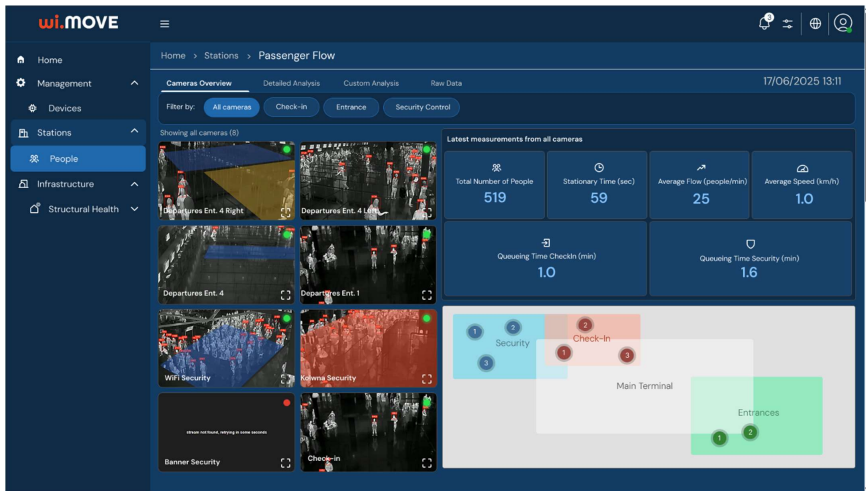
\includegraphics[width=0.9\textwidth]{antecedentes/Sistema LAP.png}
\caption{Framework de seguimiento multiobjeto basado en centroides.}
\label{fig:ant1}
\end{figure}

%% ------------------------------------------------------------
\subsection{Antecedente 2: Video-Based Pedestrian Grouping Model Considering Long-Span Space~\cite{zhao2023}}

Zhao, Wang, Jia, Li, Dong y Ma publicaron en 2023, en el \textit{Journal
of Management Science and Engineering}, un modelo de agrupamiento de
peatones evaluado en el hall del Aeropuerto Internacional de Shanghai
Hongqiao.

\begin{itemize}
    \item \textbf{Problema abordado:} los pasajeros suelen viajar en
    grupos familiares o de amigos que no siempre permanecen juntos, sino
    que pueden separarse entre 2 y 12 metros al cruzar tiendas, columnas
    u otros pasajeros. Los trackers que tratan a cada persona como una
    entidad aislada fragmentan estos grupos y distorsionan las métricas
    de flujo y congestión.

    \item \textbf{Base de datos:} video CCTV real a 10~FPS del hall del
    aeropuerto, un entorno desafiante por su alta densidad, sus
    trayectorias cruzadas en horas pico y la iluminación natural variable
    de sus ventanales.

    \item \textbf{Metodología:} el pipeline tiene cuatro componentes:
    \begin{enumerate}
        \item \textbf{Proyección homográfica:} lleva cada detección al
        plano espacial común.
        \item \textbf{MIMTrack:} seguimiento multivista que mantiene
        trayectorias consistentes entre distintas cámaras del hall.
        \item \textbf{Sequential Pattern Analysis (SPA):} identifica
        similitudes de movimiento entre trayectorias cercanas en el
        tiempo.
        \item \textbf{Grafo de conectividad PGMSL:} estima la
        probabilidad de que dos trayectorias pertenezcan a personas que
        viajan juntas.
    \end{enumerate}

    \item \textbf{Resultados:} el sistema identifica tanto grupos
    compactos como grupos separados entre 2 y 12 metros, rango que los
    sistemas anteriores ignoraban. La detección de un grupo tomó en
    promedio entre 3.21 y 4.49 segundos, compatible con un monitoreo casi
    en tiempo real, y permite derivar métricas de comportamiento grupal,
    velocidad y congestión agregada.
\end{itemize}

De este antecedente se desprende que la similitud espacial y temporal
entre trayectorias, sin señales biométricas, basta para reconstruir
estructura significativa a nivel de grupo y de multitud. Esta idea
sustenta, en el sistema propuesto, el uso de Kernel Density Estimation
para hotspots y de PrefixSpan para rutas frecuentes, ambos calculados
solo a partir de coordenadas y marcas de tiempo asociadas a un
identificador anónimo. Queda pendiente para trabajo futuro distinguir
entre viajeros individuales y grupos al calcular el tiempo de permanencia
y la tasa de captación por tienda.

\begin{figure}[H]
\centering
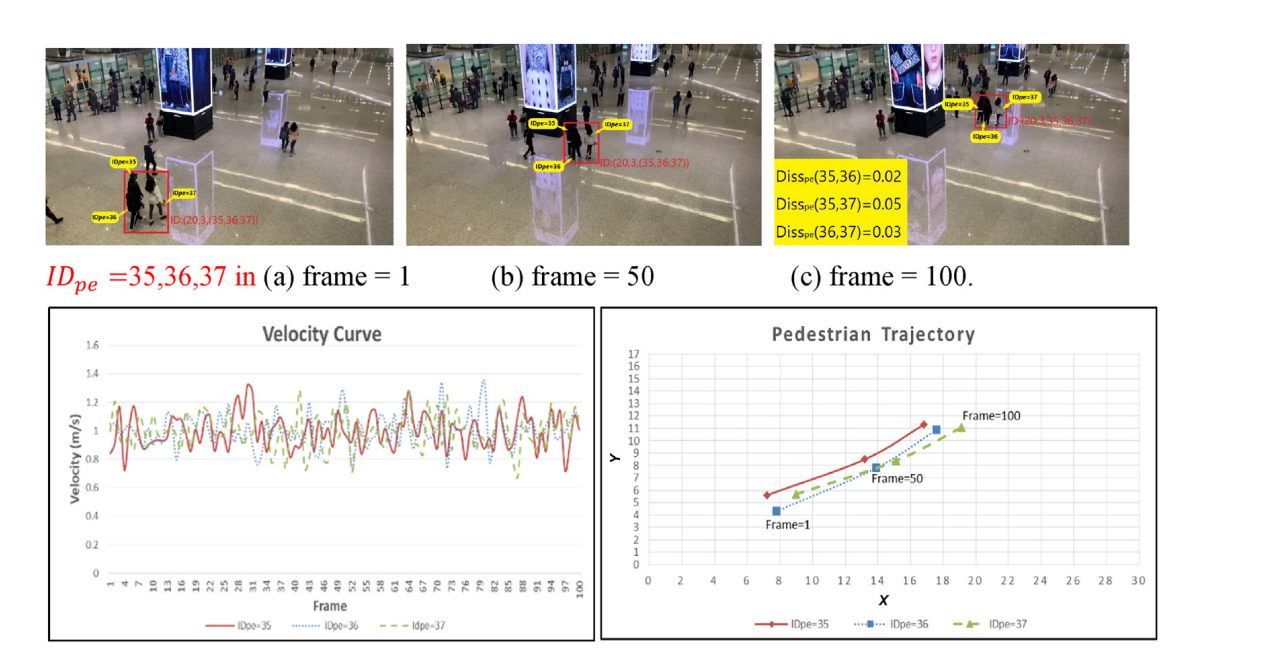
\includegraphics[width=0.9\textwidth]{antecedentes/Ant2.png}
\caption{Curva de velocidad y trayectoria de un grupo de tres peatones.}
\label{fig:ant2}
\end{figure}

%% ------------------------------------------------------------
\subsection{Antecedente 3: Multi-Camera Person Re-Identification Based on Trajectory Data~\cite{mendes2023}}

Mendes, Correia, Jorge, Brandão, Arriaga y Nunes publicaron en 2023, en
\textit{Applied Sciences}, un sistema de re-identificación multicámara
evaluado en un entorno comercial real durante siete días consecutivos.

\begin{itemize}
    \item \textbf{Problema abordado:} las cámaras existentes no comparten
    campo de visión, por lo que una misma persona recibe una identidad
    distinta en cada una; además, el reconocimiento facial es inviable
    por razones normativas y de aceptación social. Los autores proponen
    la re-identificación basada en trayectoria y apariencia como
    alternativa.

    \item \textbf{Base de datos:} 91 horas de video 1080p a 20~FPS,
    capturadas con cuatro cámaras durante siete días de operación real.

    \item \textbf{Metodología:} el pipeline tiene cuatro componentes:
    \begin{enumerate}
        \item \textbf{Detección con YOLOv5:} identifica personas en cada
        cuadro.
        \item \textbf{Tracking local con ByteTrack:} genera tracklets
        continuos por cámara.
        \item \textbf{Proyección homográfica:} lleva las posiciones a un
        plano común.
        \item \textbf{Re-identificación espacio-temporal:} combina la
        apariencia de cada tracklet con restricciones de tiempo y
        topología de cámaras, descartando asociaciones físicamente
        imposibles para no depender solo de la apariencia, que puede
        fallar ante cambios de iluminación o pose.
    \end{enumerate}

    \item \textbf{Resultados:} antes de la re-identificación había 512
    identidades, una por cada aparición en una cámara; después quedaron
    109 identidades globales frente a unas 76 personas reales, lo que
    equivale a un 82\,\% de re-identificaciones correctas y a una
    reducción de más de cuatro veces en el número de identidades.
\end{itemize}

Este es el precedente técnico más cercano al sistema propuesto, ya que
valida la combinación de un detector YOLO, un seguimiento local por
cámara y una re-identificación basada en apariencia y restricciones
espacio-temporales, que AeroVision implementa con el codificador
YOLO26s-ReID y una galería global compartida. Confirma además que el
enfoque es viable en un despliegue comercial real y respalda la decisión
de no procesar rasgos faciales. Su margen de error cercano al 18\,\%
muestra que la re-identificación sin biometría no es perfecta, por lo que
el sistema propuesto acumula muchas vistas por identidad, exige
coincidencia mutua y sin ambigüedad, y separa tracklets cuando una
fusión deja de ser coherente. La escala del experimento (cuatro cámaras,
91 horas) es, sin embargo, mucho menor que la de un aeropuerto completo.

\begin{figure}[H]
\centering
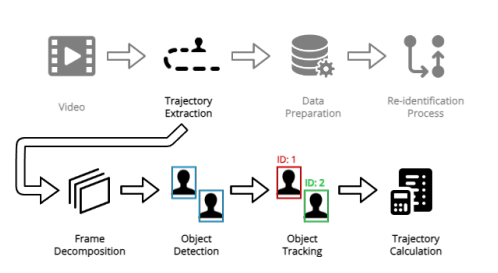
\includegraphics[width=0.9\textwidth]{antecedentes/Ant3.png}
\caption{Pipeline de extracción de trayectorias.}
\label{fig:ant3}
\end{figure}

%% ------------------------------------------------------------
\subsection{Antecedente 4: Pedestrian Attribute Recognition: MSP60K + LLM-PAR~\cite{jin2024}}

Jin, Wang, Zhu, Wang y Li publicaron en agosto de 2024, en la conferencia
AAAI, un dataset y un framework para el reconocimiento de atributos
peatonales en múltiples dominios.

\begin{itemize}
    \item \textbf{Problema abordado:} los datasets de atributos
    peatonales existentes, capturados en su mayoría en un único entorno
    controlado, generalizan mal cuando el sistema se despliega en otro
    dominio, por ejemplo al pasar de un centro comercial a un aeropuerto.

    \item \textbf{Base de datos:} MSP60K, con 60\,122 imágenes anotadas
    con 57 atributos (rango etario, género aparente, vestimenta,
    accesorios y postura), más de 5\,000 identidades y 8 escenarios
    heterogéneos, como obras de construcción, mercados, cocinas, colegios
    y espacios abiertos.

    \item \textbf{Metodología:} LLM-PAR tiene dos bloques:
    \begin{enumerate}
        \item \textbf{Codificador visual:} backbone EVA-ViT-G con un
        módulo LaRa, atención MEQFormer y bloques CBAM que refinan la
        representación de cada atributo.
        \item \textbf{Razonamiento semántico con LLM:} un modelo de
        lenguaje (Vicuna-7B u OPT-6.7B) razona sobre la compatibilidad
        entre atributos antes de la predicción final, por ejemplo,
        descartando la combinación de ``uniforme escolar'' y ``adulto
        mayor''.
    \end{enumerate}

    \item \textbf{Resultados:} F1 de 86.94 dentro del mismo dominio y
    F1 de 72.05 en evaluación entre dominios, una caída de más de 14
    puntos que los autores documentan explícitamente.
\end{itemize}

Para el sistema propuesto, este antecedente es relevante en la inferencia
demográfica aproximada: muestra que atributos generales como el rango
etario o el género aparente pueden estimarse a partir de la apariencia
corporal, sin reconocimiento facial, lo que resulta más compatible con la
Ley N.\textdegree~29733. En AeroVision esta idea se aplica, de forma
opcional, en la estimación de género por votación descrita en la
metodología. La caída de desempeño entre dominios es, sin embargo, una
advertencia: cualquier módulo demográfico deberá validarse con imágenes
del aeropuerto de Lima antes de asumir un desempeño equivalente.

\begin{figure}[H]
\centering
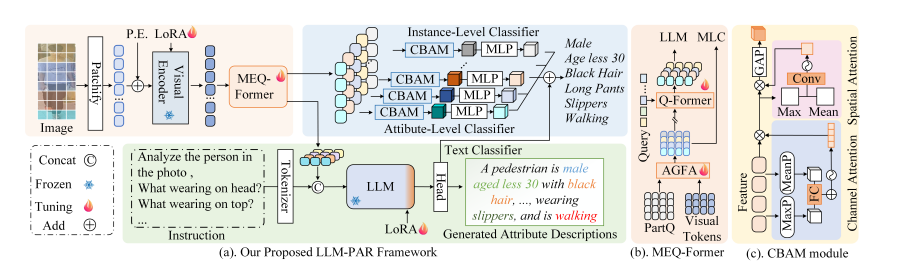
\includegraphics[width=0.9\textwidth]{antecedentes/Ant4.png}
\caption{Metodología de LLM-PAR.}
\label{fig:ant4}
\end{figure}

%% ------------------------------------------------------------
\subsection{Antecedente 5: A Unified Multi-view Multi-person Tracking Framework~\cite{yang2023}}

Yang et al., de Fujitsu Research (Japón), publicaron en 2023 un framework
unificado de tracking multivista y multipersona para generar trayectorias
globales en 3D o en vista superior a partir de varias cámaras.

\begin{itemize}
    \item \textbf{Problema abordado:} cuando cada cámara procesa sus
    detecciones sin un mecanismo de consistencia geométrica entre vistas,
    se obtienen trayectorias parciales e inconsistentes del recorrido
    real de una persona.

    \item \textbf{Base de datos:} WILDTRACK, MMPTRACK, Campus y Shelf,
    con escenas de hasta 313 personas simultáneas, 7 cámaras y más de 9.6
    horas de grabación.

    \item \textbf{Metodología:} el pipeline tiene cuatro componentes:
    \begin{enumerate}
        \item \textbf{YOLOX:} detector de personas por cámara.
        \item \textbf{Tracklets 2D por vista:} trayectorias locales
        independientes por cámara.
        \item \textbf{Distancia epipolar normalizada:} verifica si la
        posición observada en una cámara es geométricamente compatible
        con la observada en otra, dada su calibración.
        \item \textbf{PDNC y CMMT:} refinan la asociación final y la
        coherencia temporal de las trayectorias globales.
    \end{enumerate}

    \item \textbf{Resultados:} MOTA de 95.2\,\% e IDF1 de 97.5\,\% en
    WILDTRACK; MOTA de 95\,\% e IDF1 de 84.3\,\% a 67~FPS en MMPTRACK,
    entre los valores más altos de los antecedentes revisados.
\end{itemize}

Este antecedente valida la etapa de mapeo sobre un plano común: la
verificación geométrica entre vistas complementa la asociación por
apariencia al unificar detecciones de varias cámaras. Sus altos valores
de MOTA e IDF1 en escenas con más de 300 personas respaldan la
factibilidad de un seguimiento multicámara de calidad en horas pico. No
obstante, WILDTRACK y MMPTRACK son espacios relativamente controlados,
distintos de una terminal con mobiliario, equipaje y señalética, por lo
que el sistema propuesto debe validar estas métricas con datos propios.
En AeroVision, este tipo de verificación geométrica se activa en el modo
calibrado, cuando las homografías de las cámaras están validadas.

\begin{figure}[H]
\centering
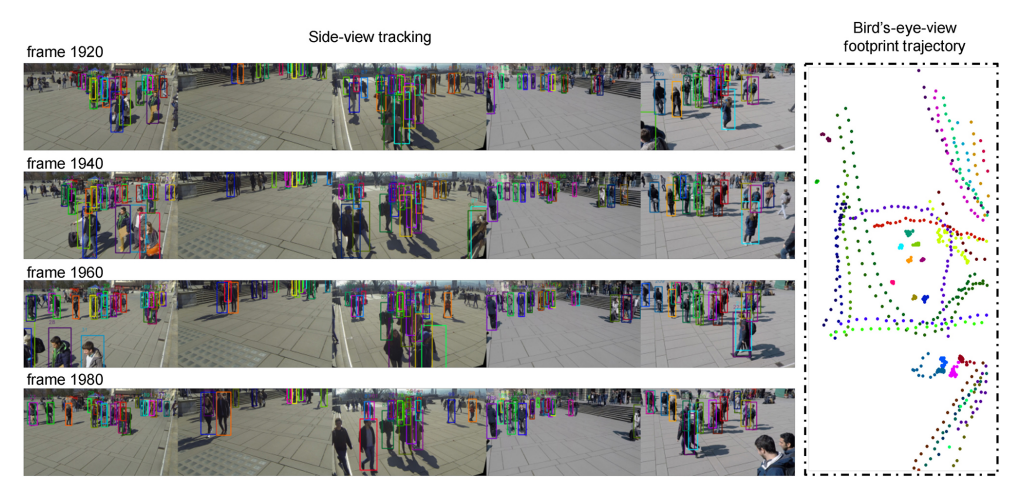
\includegraphics[width=0.9\textwidth]{antecedentes/Ant5.png}
\caption{Resultados del tracking en el conjunto de prueba.}
\label{fig:ant5}
\end{figure}

%% ------------------------------------------------------------
\subsection{Antecedente 6: Event Detection in Videos: A Framework for the Development of New Methods~\cite{zakharova2026}}

Zakharova, Bouwmans, Cioppa y colaboradores, de La Rochelle University y
otras instituciones, publicaron en arXiv, en julio de 2026, un framework
general para definir y evaluar eventos detectados en video.

\begin{itemize}
    \item \textbf{Problema abordado:} cada sistema de detección de
    eventos define ``evento'' a su manera y lo evalúa con métricas
    propias, lo que impide comparar métodos.

    \item \textbf{Base de datos:} FSD, con 43 cámaras IP y 153\,191
    cuadros anotados con máscaras de primer plano, y SUC, con 187\,500
    cuadros de 6 cámaras, ambos con peatones en movimiento, cambios
    bruscos de iluminación, objetos pequeños y visión nocturna.

    \item \textbf{Metodología:} se propone evaluar la detección de
    eventos en tres niveles:
    \begin{enumerate}
        \item \textbf{Píxel:} si cada píxel se clasificó correctamente
        como parte de un evento.
        \item \textbf{Cuadro:} si el cuadro completo refleja el evento
        esperado.
        \item \textbf{Segmento temporal:} si el evento se detecta a lo
        largo de una ventana de tiempo.
    \end{enumerate}
    En cada nivel se calculan precisión, recall, F1 e IoU de forma
    estandarizada.

    \item \textbf{Resultados:} en lugar de un único valor de desempeño,
    el trabajo valida el propio framework sobre FSD y SUC y demuestra que
    la evaluación multigranular es aplicable de forma consistente.
\end{itemize}

El motor de eventos del sistema propuesto (EXPOSURE, ENTER, DWELL, EXIT,
RETURN y QUEUE) se beneficia de este criterio: conviene evaluar cada tipo
de evento en distintas granularidades temporales en lugar de reportar una
sola métrica agregada, especialmente ante la iluminación variable y los
objetos pequeños propios de una terminal. Por su publicación reciente,
estas métricas aún no tienen adopción amplia, por lo que su uso en este
trabajo es una decisión metodológica temprana.

\begin{figure}[H]
\centering
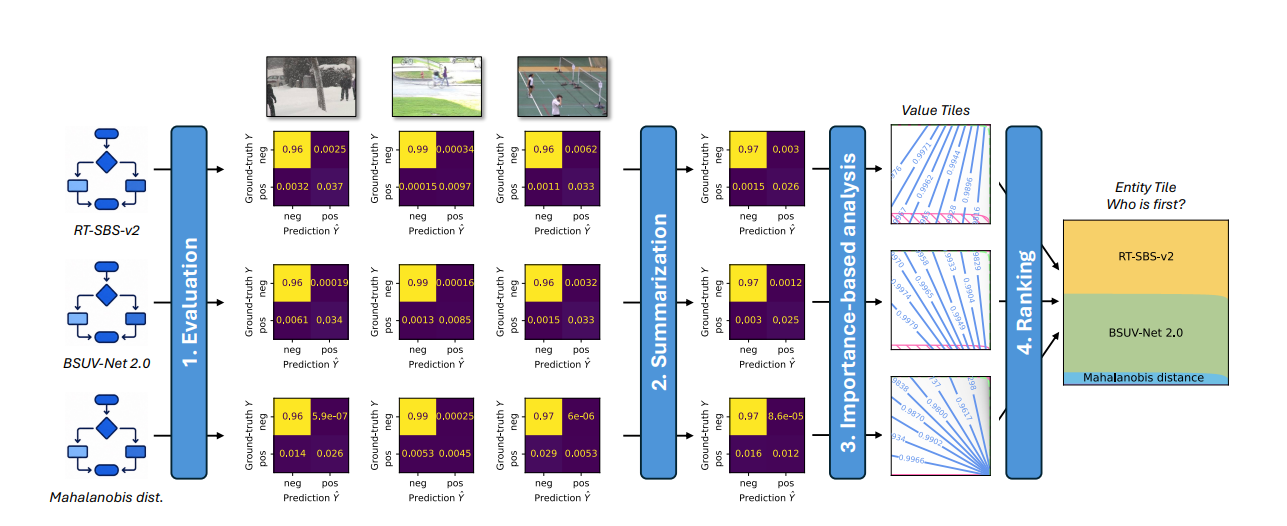
\includegraphics[width=0.9\textwidth]{antecedentes/ant6.png}
\caption{Pipeline de evaluación de eventos.}
\label{fig:ant6}
\end{figure}

%% ------------------------------------------------------------
\subsection{Antecedente 7: Beyond Social Distancing: Application of Real-World Coordinates in a Multi-Camera System with Privacy Protection~\cite{ryan2023}}

Ryan y su equipo, de Stanford University, publicaron en 2023 un sistema
multicámara evaluado en un aeropuerto operativo de Dublín.

\begin{itemize}
    \item \textbf{Problema abordado:} construir una representación
    espacial unificada del movimiento de las personas en la terminal sin
    identificadores biométricos ni reconocimiento facial, dado que el
    sistema opera sobre CCTV en producción con pasajeros que no dieron
    consentimiento explícito.

    \item \textbf{Base de datos:} CCTV real de un aeropuerto de Dublín;
    el trabajo no especifica las horas de video ni el número de cámaras
    de la evaluación.

    \item \textbf{Metodología:} el pipeline tiene cuatro componentes:
    \begin{enumerate}
        \item \textbf{YOLOv5x:} detección de personas.
        \item \textbf{DeepSORT:} seguimiento local por cámara.
        \item \textbf{Transformación de perspectiva:} proyección sobre un
        plano común.
        \item \textbf{Re-identificación por distancia coseno:} asignación
        entre tracklets de distintas cámaras con el algoritmo húngaro.
    \end{enumerate}

    \item \textbf{Resultados:} trayectorias globales consistentes entre
    cámaras, integradas con un sistema GIS del aeropuerto, y una
    validación cualitativa, sin métricas cuantitativas de MOTA o IDF1.
\end{itemize}

Este antecedente fue evaluado en un aeropuerto real, por lo que confirma
que la combinación de detección, seguimiento local, proyección y
re-identificación sin biometría es viable en este dominio. Respalda la
proyección de las posiciones sobre un plano 2D común del aeropuerto Jorge
Chávez y su integración con un mapa. La ausencia de métricas
cuantitativas deja una laguna que el sistema propuesto busca cubrir
reportando precisión, recall e IDF1 con datos etiquetados.

\begin{figure}[H]
\centering
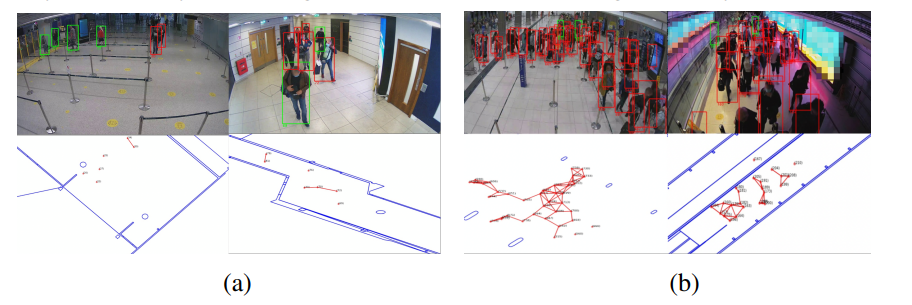
\includegraphics[width=0.9\textwidth]{antecedentes/Ant7.png}
\caption{a) Casos de éxito; b) casos fallidos por exceso de personas.}
\label{fig:ant7}
\end{figure}

%% ------------------------------------------------------------
\subsection{Antecedente 8: Fusion of CCTV Video and Spatial Information for Automated Crowd Congestion Monitoring in Public Urban Spaces~\cite{wonglaw2023}}

Wong y Law, también de Stanford University, publicaron en 2023 un sistema
que fusiona video CCTV con información espacial del entorno.

\begin{itemize}
    \item \textbf{Problema abordado:} la mayoría de sistemas de monitoreo
    de multitudes reporta solo la densidad instantánea por cámara, sin
    una vista agregada del espacio ni capacidad para predecir la
    congestión de los minutos siguientes.

    \item \textbf{Base de datos:} datos de Grand Central Station y del
    Stanford Stadium, con 17\,682 trayectorias sobre 6\,000 cuadros.

    \item \textbf{Metodología:} el pipeline tiene cinco componentes:
    \begin{enumerate}
        \item \textbf{YOLOv7-tiny:} detección de personas.
        \item \textbf{DeepSORT:} seguimiento local.
        \item \textbf{Homografía:} proyección sobre el plano del espacio.
        \item \textbf{CMGraph:} grafo de conectividad entre zonas.
        \item \textbf{GCN + GRU:} modelado temporal del flujo entre zonas
        para predecir la congestión futura.
    \end{enumerate}

    \item \textbf{Resultados:} MOTA de 73.7\,\%, MODA de 81.2\,\%, recall
    de 86.2\,\%, precisión de 94.6\,\%, y predicción de flujo con MSE de
    0.258 y MAE de 0.354; su tracking es más modesto que el de Yang et
    al.~\cite{yang2023}, pero es el único antecedente con capacidad
    predictiva.
\end{itemize}

Este antecedente aporta directamente al módulo de flujo entre zonas del
sistema propuesto. Representar el espacio como un grafo de zonas
conectadas permite generar mapas de calor y métricas de flujo, y admite
la predicción de congestión, que queda como trabajo futuro, ya que el
sistema propuesto reporta por ahora la congestión observada.

\begin{figure}[H]
\centering
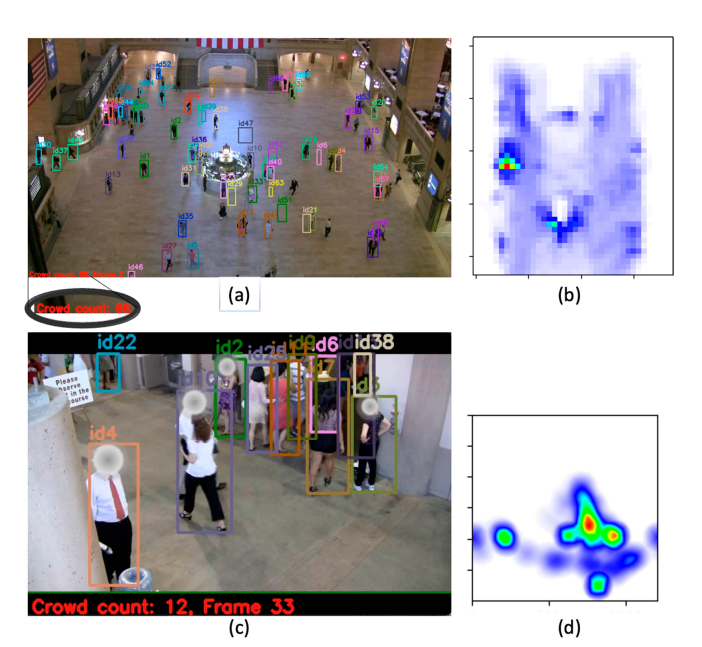
\includegraphics[width=0.9\textwidth]{antecedentes/Ant8.png}
\caption{Visualización de aglomeraciones en la estación.}
\label{fig:ant8}
\end{figure}

%% ------------------------------------------------------------
\subsection{Antecedente 9: Real-Time Pedestrian Detection and Multi-Object Tracking in Complex Airport Scenes via Frequency-Aware and Mamba-Enhanced Representation~\cite{zhou2026}}

Zhou y su equipo, en colaboración entre Chongqing y Nanjing Airlines
(China), publicaron en 2026 un tracker especializado para escenas
aeroportuarias.

\begin{itemize}
    \item \textbf{Problema abordado:} los trackers genéricos, evaluados
    sobre escenas urbanas o de vigilancia convencional, pierden
    desempeño en terminales aeroportuarias, donde la densidad, el
    equipaje, los cambios de iluminación y las oclusiones son más
    adversos que en los benchmarks estándar.

    \item \textbf{Base de datos:} AirportPassenger, dataset privado con
    12\,000 imágenes y 285\,000 instancias anotadas de pasajeros en
    escenas aeroportuarias reales.

    \item \textbf{Metodología:} AirMOTR incorpora dos componentes:
    \begin{enumerate}
        \item \textbf{Representaciones sensibles a la frecuencia:}
        capturan texturas y bordes que ayudan a distinguir personas entre
        equipaje y mobiliario.
        \item \textbf{Bloques Mamba:} modelos de espacio de estados, más
        eficientes que la atención estándar, para dependencias temporales
        largas.
    \end{enumerate}
    El modelo se comparó con DeepSORT, ByteTrack, BoT-SORT y MOTR sobre
    el mismo dataset.

    \item \textbf{Resultados:} AirMOTR obtuvo MOTA de 79.6\,\%, IDF1 de
    84.2\,\% y 41.6~FPS, superando a ByteTrack, segundo mejor, con MOTA
    de 72.3\,\%, IDF1 de 76.82\,\% y 42.5~FPS.
\end{itemize}

Este es el antecedente más cercano al dominio de aplicación, pues fue
evaluado en escenas aeroportuarias complejas. Muestra que los trackers
genéricos, incluido ByteTrack, ofrecen un desempeño sólido pero
mejorable en este dominio. La diferencia de 7.3 puntos de MOTA sugiere
que migrar a una arquitectura especializada no sería decisivo a corto
plazo, lo que justifica un seguidor local liviano cuya asociación en dos
etapas se inspira en ByteTrack, reforzado con apariencia corporal y
memoria visual para los cruces y oclusiones. La evaluación de
arquitecturas como AirMOTR queda como trabajo futuro, cuando se disponga
de suficientes datos propios.

\begin{figure}[H]
\centering
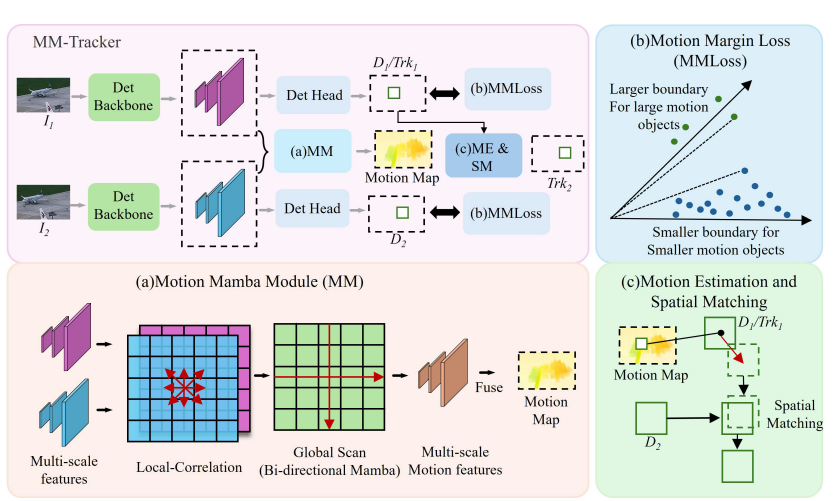
\includegraphics[width=0.9\textwidth]{antecedentes/Ant9.png}
\caption{Estructura del pipeline de seguimiento.}
\label{fig:ant9}
\end{figure}

%% ------------------------------------------------------------
\subsection{Cuadro Comparativo de Antecedentes}

El Cuadro~\ref{tab:antecedentes} resume las métricas principales, el
dominio de evaluación y el aporte de cada antecedente al sistema
propuesto.

\begin{table}[t]
\centering
\caption{Resumen comparativo de los nueve antecedentes revisados.}
\label{tab:antecedentes}
\begin{tabular}{@{}p{3.2cm}p{2.8cm}p{3cm}p{6.5cm}@{}}
\toprule
\textbf{Antecedente} & \textbf{Dominio de evaluación} & \textbf{Métrica clave} & \textbf{Aporte al sistema propuesto} \\
\midrule
Giannopoulou et al.~\cite{giannopoulou2026} & Aeropuerto real (Atenas) & mAP 0.87; 100\,\% de fiabilidad & Respalda un detector YOLO y un seguimiento local liviano en arquitectura modular \\
Zhao et al.~\cite{zhao2023} & Aeropuerto real (Shanghai) & Detección de grupo en 3.21--4.49~s & Sustenta KDE y PrefixSpan en la minería de patrones \\
Mendes et al.~\cite{mendes2023} & Entorno comercial real & 82\,\% de re-ID correcta & Precedente directo de la re-identificación multicámara sin rostro \\
Jin et al.~\cite{jin2024} & 8 dominios (MSP60K) & F1 86.94 / 72.05 entre dominios & Habilita inferencia demográfica sin biometría \\
Yang et al.~\cite{yang2023} & WILDTRACK / MMPTRACK & MOTA 95.2\,\% & Valida la verificación geométrica sobre un plano común \\
Zakharova et al.~\cite{zakharova2026} & FSD / SUC (CCTV real) & Evaluación multigranular & Criterio para evaluar el motor de eventos \\
Ryan et al.~\cite{ryan2023} & Aeropuerto real (Dublín) & Cualitativo (sin MOTA) & Valida la arquitectura completa en el dominio aeroportuario \\
Wong y Law~\cite{wonglaw2023} & Grand Central / Stanford Stadium & MOTA 73.7\,\%; MSE 0.258 & Grafo origen-destino y predicción de congestión futura \\
Zhou et al.~\cite{zhou2026} & Aeropuerto (AirportPassenger) & MOTA 79.6\,\% (AirMOTR) & Referencia para especializar el seguimiento local \\
\bottomrule
\end{tabular}
\end{table}

\FloatBarrier

%% ------------------------------------------------------------
\subsection{Síntesis y Vacío de Investigación}

Tomados en conjunto, los nueve antecedentes muestran que cada pieza
técnica del problema (detección, seguimiento, re-identificación sin
biometría, mapeo espacial, minería de patrones e insights comerciales) ha
sido resuelta por separado, varias veces incluso en aeropuertos reales
(Atenas, Shanghai Hongqiao, Dublín y las escenas de AirportPassenger),
pero ningún trabajo las integra en un solo pipeline desplegable bajo un
marco ético adecuado al contexto regulatorio latinoamericano. El aporte
de cada antecedente es el siguiente:

\begin{itemize}
    \item \textbf{Giannopoulou et al.~\cite{giannopoulou2026}} muestra,
    con 42.9~ms de latencia y 100\,\% de fiabilidad, que un pipeline
    ligero sostiene monitoreo continuo a escala de terminal, lo que
    respalda un detector YOLO, un seguidor local liviano y una
    arquitectura modular en contenedores.

    \item \textbf{Zhao et al.~\cite{zhao2023}} demuestra que el
    comportamiento de grupos separados hasta 12 metros puede
    reconstruirse con similitud espacio-temporal, lo que sustenta KDE y
    PrefixSpan.

    \item \textbf{Mendes et al.~\cite{mendes2023}} valida, al reducir 512
    identidades a 109, la re-identificación por apariencia y restricciones
    espacio-temporales; su 18\,\% de error justifica acumular muchas
    vistas por identidad y exigir coincidencias mutuas y sin ambigüedad.

    \item \textbf{Jin et al.~\cite{jin2024}} confirma que la inferencia
    de atributos demográficos es posible sin biometría, y su caída entre
    dominios obliga a validar ese módulo con datos propios.

    \item \textbf{Yang et al.~\cite{yang2023}} valida que la verificación
    geométrica entre vistas complementa la apariencia en escenas densas,
    lo que respalda el modo calibrado y el mapeo por homografía.

    \item \textbf{Zakharova et al.~\cite{zakharova2026}} aporta un
    criterio para evaluar el motor de eventos en varias granularidades.

    \item \textbf{Ryan et al.~\cite{ryan2023}} confirma, en un aeropuerto
    real, la viabilidad de la arquitectura completa y de su integración
    con un mapa 2D.

    \item \textbf{Wong y Law~\cite{wonglaw2023}} demuestra que un grafo de
    zonas permite mapas de calor, métricas de flujo y, a futuro,
    predicción de congestión.

    \item \textbf{Zhou et al.~\cite{zhou2026}} muestra que ByteTrack es
    sólido pero mejorable en aeropuertos, lo que motiva reforzar el
    seguimiento local con apariencia y memoria visual, y evaluar AirMOTR a
    futuro.
\end{itemize}

El vacío que aborda este trabajo es, por tanto, más amplio que el de
cualquier antecedente aislado, pero más concreto que el de un sistema
comercial genérico. El prototipo integra YOLO26m para la detección, un
seguidor local híbrido con memoria visual, el codificador YOLO26s-ReID y
una galería global compartida para la re-identificación sin biometría,
homografía para el mapeo sobre un plano 2D común, un motor de eventos con
minería de patrones (KDE, PrefixSpan y grafo origen-destino) y un
dashboard de insights, desplegados con un servicio de visión en Python,
un backend en Go, PostgreSQL/PostGIS y Vue.js. La predicción de
congestión, la especialización del seguimiento con arquitecturas tipo
AirMOTR y el clasificador de edad para la exclusión de menores no se
presentan como componentes implementados, sino como trabajo futuro.

%% ============================================================
%% V. Especificación de Requerimientos
%% ============================================================

\section{Especificación de Requerimientos}

\subsection{Casos de Uso del Sistema}

Esta sección presenta los casos de uso del sistema, que describen cómo cada
actor interactúa con las funciones definidas en los requerimientos
funcionales. Cada caso de uso indica su actor principal, el requerimiento
que cubre, su historia de usuario, precondiciones, flujo principal, flujos
alternativos y postcondiciones. El sistema tiene dos actores: el
\textbf{Usuario comercial}, que consulta el análisis y los insights, y el
\textbf{Usuario administrador}, que monitorea, configura el mapa y procesa
los videos. Ambos roles se registran en la tabla \texttt{roles} de la base
de datos.

% ------------------------------------------------------------
\textbf{CU-01: Iniciar y cerrar sesión}

\textbf{Actor principal:} Usuario comercial, Usuario administrador \\
\textbf{Requerimiento:} RF-01

\textbf{Historia de usuario:} Como usuario del sistema, quiero iniciar sesión con mis credenciales y cerrarla al terminar, para acceder de forma segura solo a las funciones permitidas por mi rol.

\textbf{Precondiciones:} El usuario está registrado y activo.

\textbf{Flujo principal:}
\begin{enumerate}
    \item El usuario ingresa su usuario y contraseña.
    \item El sistema valida las credenciales y el rol.
    \item El sistema redirige a la vista permitida para su rol.
    \item Al pulsar ``Cerrar sesión'', el sistema invalida la sesión.
\end{enumerate}

\textbf{Flujos alternativos:} Si las credenciales son inválidas, el sistema
muestra un error; tras varios intentos fallidos, bloquea el acceso
temporalmente.

\textbf{Postcondiciones:} Sesión activa con los permisos del rol, o sesión cerrada.

\begin{figure}[H]
\centering
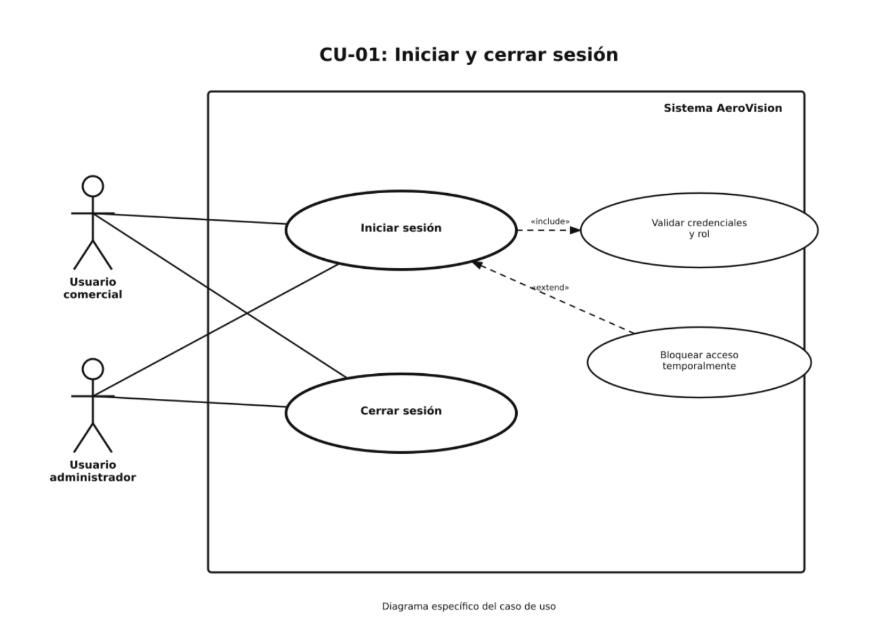
\includegraphics[width=0.85\columnwidth]{CasosdeUSO/1.png}
\caption{CU-01: Iniciar y cerrar sesión}
\label{fig:cu01}
\end{figure}

% ------------------------------------------------------------
\textbf{CU-02: Monitorear personas y trayectorias en vivo}

\textbf{Actor principal:} Usuario administrador \\
\textbf{Requerimiento:} RF-02

\textbf{Historia de usuario:} Como usuario administrador, quiero visualizar en tiempo real a las personas y sus trayectorias sobre el plano del aeropuerto, para conocer el estado de la operación y actuar ante aglomeraciones o incidencias.

\textbf{Precondiciones:} Sesión iniciada, plano y zonas configurados, y
trayectorias disponibles.

\textbf{Flujo principal:}
\begin{enumerate}
    \item El usuario accede a la pantalla ``Mapa''.
    \item El sistema muestra el plano 2D con las personas, su estado y su zona.
    \item El usuario activa las capas de trayectorias, zonas o cámaras.
    \item El usuario selecciona una persona.
    \item El sistema aísla su recorrido y sus eventos.
\end{enumerate}

\textbf{Flujos alternativos:} Si no hay datos en la ventana, el sistema
muestra el aviso ``sin observaciones''.

\textbf{Postcondiciones:} Estado actual del aeropuerto visible con
identificadores anónimos.

\begin{figure}[H]
\centering
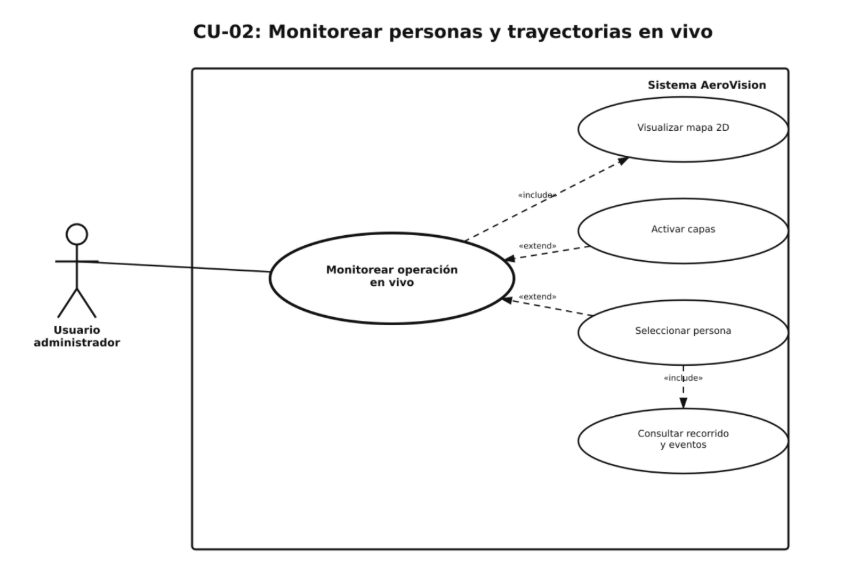
\includegraphics[width=0.85\columnwidth]{CasosdeUSO/2.png}
\caption{CU-02: Monitorear personas y trayectorias en vivo}
\label{fig:cu02}
\end{figure}

% ------------------------------------------------------------
\textbf{CU-03: Reproducir histórico de movimiento}

\textbf{Actor principal:} Usuario comercial, Usuario administrador \\
\textbf{Requerimiento:} RF-04

\textbf{Historia de usuario:} Como usuario del sistema, quiero reproducir el movimiento histórico de las personas en un periodo específico, para entender cómo se comportó el flujo en un momento pasado.

\textbf{Precondiciones:} Existen posiciones registradas en el periodo.

\textbf{Flujo principal:}
\begin{enumerate}
    \item El usuario elige la ventana temporal.
    \item El sistema carga la reproducción.
    \item El usuario reproduce, pausa, arrastra la línea de tiempo o cambia la velocidad.
    \item El sistema recalcula los indicadores en el instante reproducido.
\end{enumerate}

\textbf{Flujos alternativos:} Si el filtro es inválido, el sistema lo
rechaza con un mensaje.

\textbf{Postcondiciones:} Movimiento del periodo reproducido junto con sus métricas.

\begin{figure}[H]
\centering
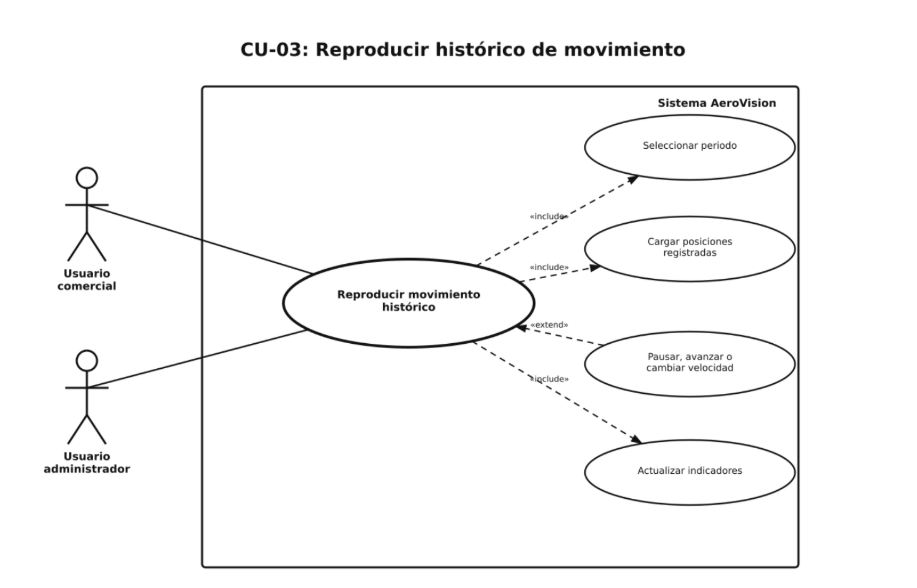
\includegraphics[width=0.85\columnwidth]{CasosdeUSO/3.png}
\caption{CU-03: Reproducir histórico de movimiento}
\label{fig:cu03}
\end{figure}

% ------------------------------------------------------------
\textbf{CU-04: Configurar zonas del mapa}

\textbf{Actor principal:} Usuario administrador \\
\textbf{Requerimiento:} RF-03

\textbf{Historia de usuario:} Como usuario administrador, quiero crear, modificar y eliminar zonas sobre el plano, para reflejar en el sistema la distribución real de puestos y áreas del aeropuerto.

\textbf{Precondiciones:} Sesión de usuario administrador en la pantalla ``Configuración''.

\textbf{Flujo principal:}
\begin{enumerate}
    \item El usuario pulsa ``Puesto/zona''.
    \item El usuario marca los vértices y cierra el polígono.
    \item El usuario define nombre, tipo y color.
    \item El usuario guarda los cambios.
    \item El sistema valida y registra la zona.
\end{enumerate}

\textbf{Flujos alternativos:} Si cancela, se descarta el borrador. Si la
geometría es inválida o la zona fue modificada por otro usuario, el sistema
rechaza el cambio. Para eliminar una zona, el sistema pide confirmación.

\textbf{Postcondiciones:} Zona disponible en el mapa y en los insights.

\begin{figure}[H]
\centering
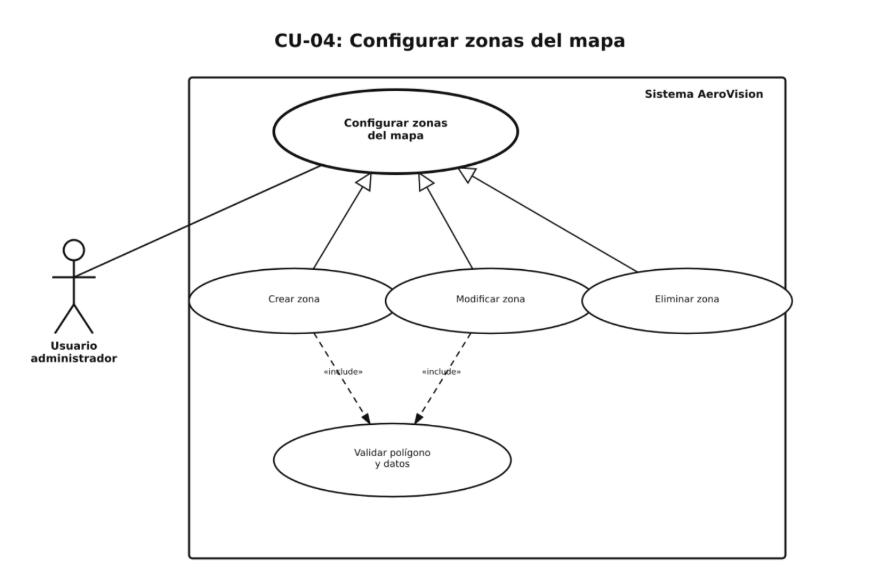
\includegraphics[width=0.85\columnwidth]{CasosdeUSO/4.png}
\caption{CU-04: Configurar zonas del mapa}
\label{fig:cu04}
\end{figure}
% ------------------------------------------------------------
\textbf{CU-05: Configurar cámaras y cobertura}

\textbf{Actor principal:} Usuario administrador \\
\textbf{Requerimiento:} RF-03

\textbf{Historia de usuario:} Como usuario administrador, quiero ubicar las cámaras en el plano y definir su área de cobertura, para que el sistema sepa qué zona física observa cada una.

\textbf{Precondiciones:} Sesión de usuario administrador en la pantalla ``Configuración''.

\textbf{Flujo principal:}
\begin{enumerate}
    \item El usuario pulsa ``Asignar cámara'' y marca su ubicación.
    \item El usuario define nombre, fuente, color y orientación.
    \item El usuario dibuja el área de cobertura.
    \item El usuario guarda los cambios.
\end{enumerate}

\textbf{Flujos alternativos:} El usuario puede arrastrar los vértices para
ajustar la cobertura. Un dispositivo ya asignado a otra cámara no aparece
como opción.

\textbf{Postcondiciones:} Cámara y cobertura registradas en el plano.

\begin{figure}[H]
\centering
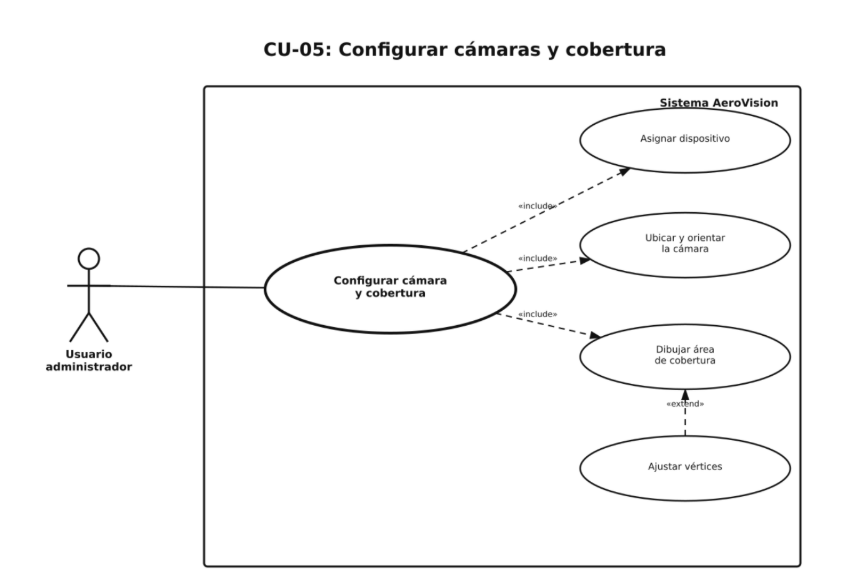
\includegraphics[width=0.85\columnwidth]{CasosdeUSO/5.png}
\caption{CU-05: Configurar cámaras y cobertura}
\label{fig:cu05}
\end{figure}

% ------------------------------------------------------------
\textbf{CU-06: Ver cámara en vivo}

\textbf{Actor principal:} Usuario administrador \\
\textbf{Requerimiento:} RF-02

\textbf{Historia de usuario:} Como usuario administrador, quiero ver el video en vivo de una cámara asignada, para verificar directamente lo que ocurre en una zona específica.

\textbf{Precondiciones:} Cámara con dispositivo asignado y acceso seguro al sistema.

\textbf{Flujo principal:}
\begin{enumerate}
    \item El usuario selecciona la cámara.
    \item El usuario pulsa ``Activar cámara'' y concede el permiso del navegador.
    \item El sistema muestra el video y el movimiento detectado.
    \item El usuario pulsa ``Detener''.
\end{enumerate}

\textbf{Flujos alternativos:} Si no hay dispositivo asignado o se deniega el
permiso, el sistema muestra un aviso y deshabilita la activación.

\textbf{Postcondiciones:} Cámara liberada al detener o al salir de la pantalla.

\begin{figure}[H]
\centering
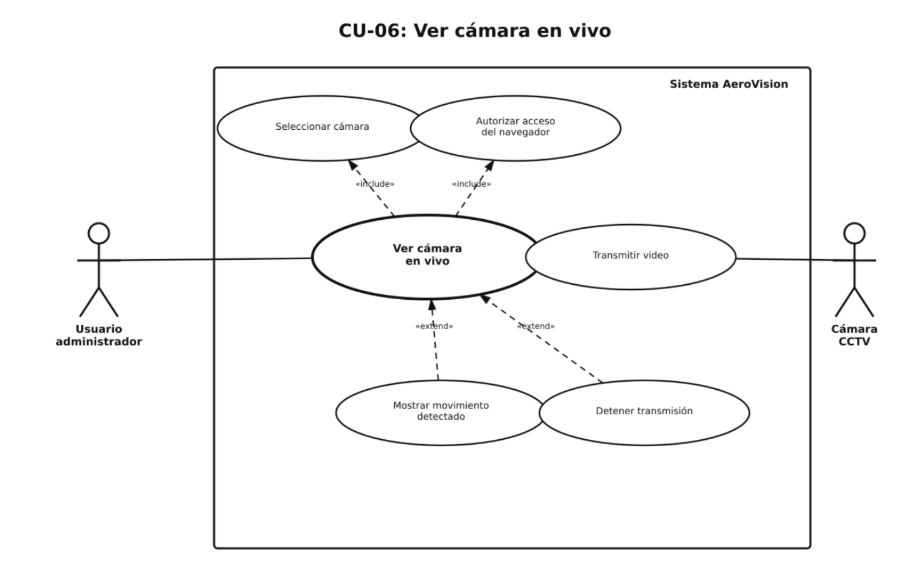
\includegraphics[width=0.85\columnwidth]{CasosdeUSO/6.png}
\caption{CU-06: Ver cámara en vivo}
\label{fig:cu06}
\end{figure}

% ------------------------------------------------------------
\textbf{CU-07: Consultar mapa de calor}

\textbf{Actor principal:} Usuario comercial \\
\textbf{Requerimiento:} RF-04

\textbf{Historia de usuario:} Como usuario comercial, quiero visualizar un mapa de calor de las zonas con mayor aglomeración en un periodo, para identificar los puntos de mayor tránsito y tomar decisiones comerciales informadas.

\textbf{Precondiciones:} Existen posiciones históricas registradas.

\textbf{Flujo principal:}
\begin{enumerate}
    \item El usuario accede a la pantalla ``Insights''.
    \item El usuario selecciona el periodo.
    \item El sistema superpone el mapa de calor sobre el plano con su leyenda.
\end{enumerate}

\textbf{Flujos alternativos:} Si el periodo no tiene datos, el sistema
muestra el mapa vacío con un aviso.

\textbf{Postcondiciones:} Zonas de mayor aglomeración identificadas.

\begin{figure}[H]
\centering
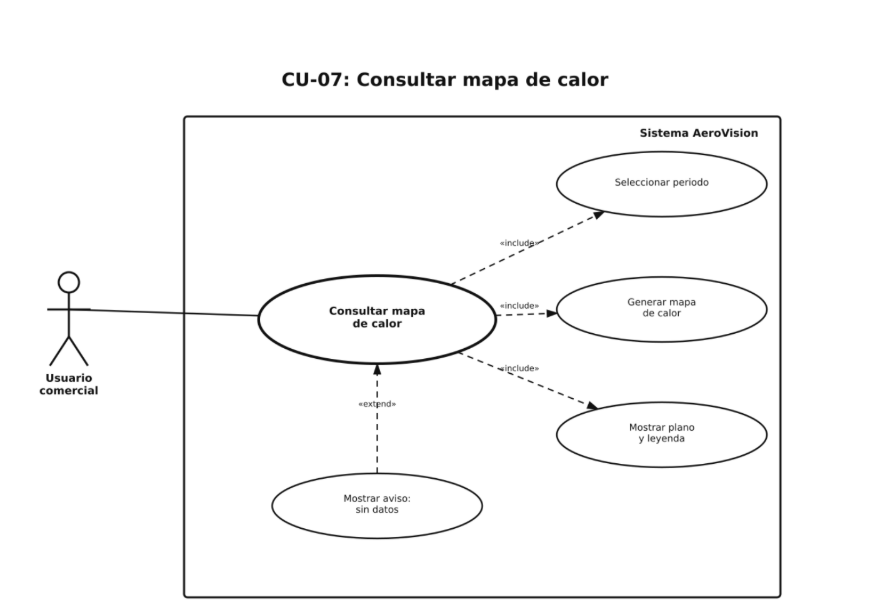
\includegraphics[width=0.85\columnwidth]{CasosdeUSO/7.png}
\caption{CU-07: Consultar mapa de calor}
\label{fig:cu07}
\end{figure}


% ------------------------------------------------------------
\textbf{CU-08: Consultar insights por zona}

\textbf{Actor principal:} Usuario comercial \\
\textbf{Requerimiento:} RF-05

\textbf{Historia de usuario:} Como usuario comercial, quiero consultar las visitas, la permanencia y la captación por zona y periodo, para evaluar el desempeño de cada punto comercial y comparar su evolución.

\textbf{Precondiciones:} Zonas configuradas y visitas registradas.

\textbf{Flujo principal:}
\begin{enumerate}
    \item El usuario accede a la pantalla ``Insights''.
    \item El usuario selecciona el periodo y la zona.
    \item El sistema muestra visitas, pass-by, permanencia, captación, densidad y su evolución en el tiempo.
\end{enumerate}

\textbf{Flujos alternativos:} El usuario puede comparar dos periodos.

\textbf{Postcondiciones:} Métricas agregadas por zona sin datos personales.

\begin{figure}[H]
\centering
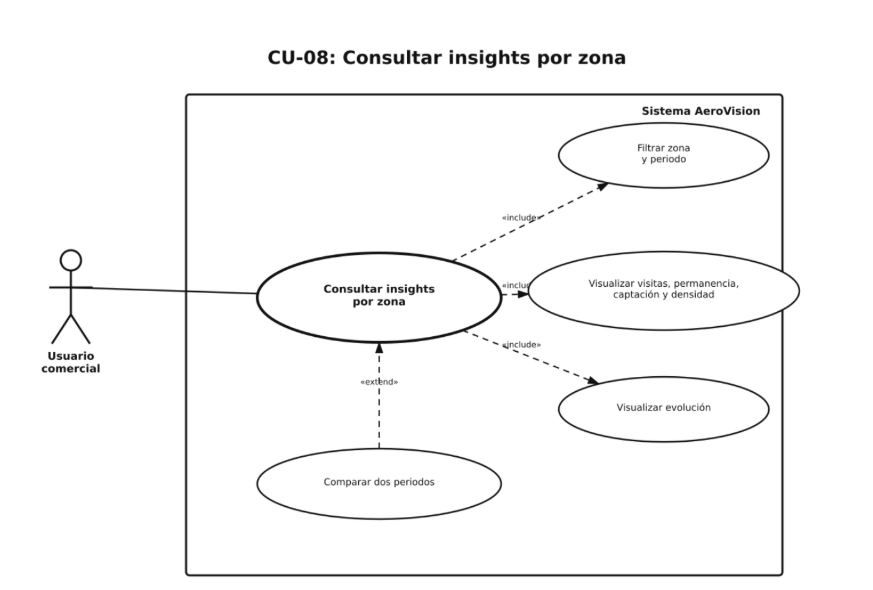
\includegraphics[width=0.85\columnwidth]{CasosdeUSO/8.png}
\caption{CU-08: Consultar insights por zona}
\label{fig:cu08}
\end{figure}
% ------------------------------------------------------------
\textbf{CU-09: Analizar flujos entre zonas}

\textbf{Actor principal:} Usuario comercial \\
\textbf{Requerimiento:} RF-04

\textbf{Historia de usuario:} Como usuario comercial, quiero visualizar los flujos de personas entre zonas y su volumen, para entender las rutas más frecuentes y optimizar la ubicación de los puntos comerciales.

\textbf{Precondiciones:} Existen entradas y salidas de zonas registradas.

\textbf{Flujo principal:}
\begin{enumerate}
    \item El usuario activa la capa de flujos.
    \item El sistema dibuja las transiciones de origen a destino con su volumen.
\end{enumerate}

\textbf{Flujos alternativos:} Si no hay transiciones en el periodo, el
sistema muestra un aviso.

\textbf{Postcondiciones:} Rutas más frecuentes entre zonas visibles.

\begin{figure}[H]
\centering
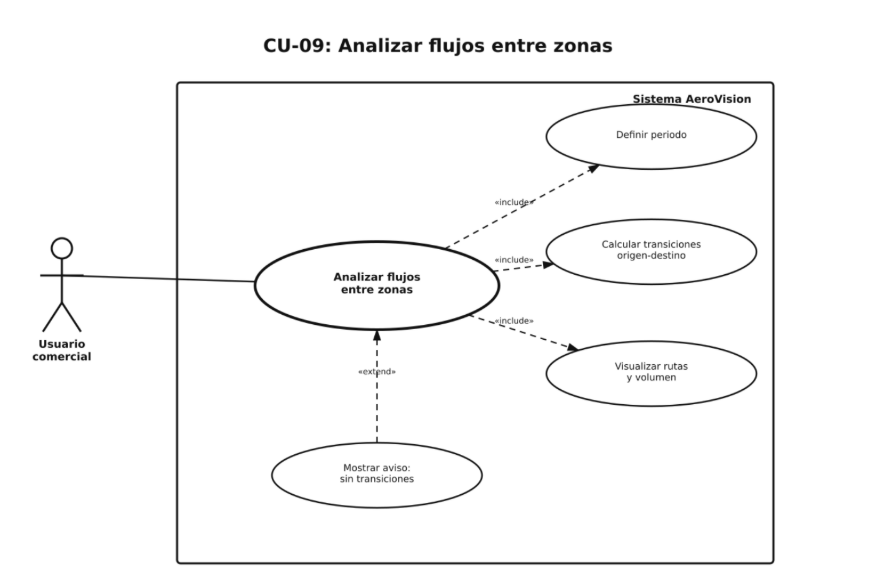
\includegraphics[width=0.85\columnwidth]{CasosdeUSO/9.png}
\caption{CU-09: Analizar flujos entre zonas}
\label{fig:cu09}
\end{figure}

% ------------------------------------------------------------
\textbf{CU-10: Exportar reporte}

\textbf{Actor principal:} Usuario comercial \\
\textbf{Requerimiento:} RF-05

\textbf{Historia de usuario:} Como usuario comercial, quiero exportar los insights de un periodo en CSV o PDF, para compartir los resultados con mi equipo o usarlos fuera del sistema.

\textbf{Precondiciones:} Insights cargados para un periodo.

\textbf{Flujo principal:}
\begin{enumerate}
    \item El usuario pulsa ``Exportar''.
    \item El usuario elige el formato CSV o PDF.
    \item El sistema genera y descarga el archivo.
\end{enumerate}

\textbf{Flujos alternativos:} Si la generación es prolongada, el sistema
muestra el progreso.

\textbf{Postcondiciones:} Reporte descargado.

\begin{figure}[H]
\centering
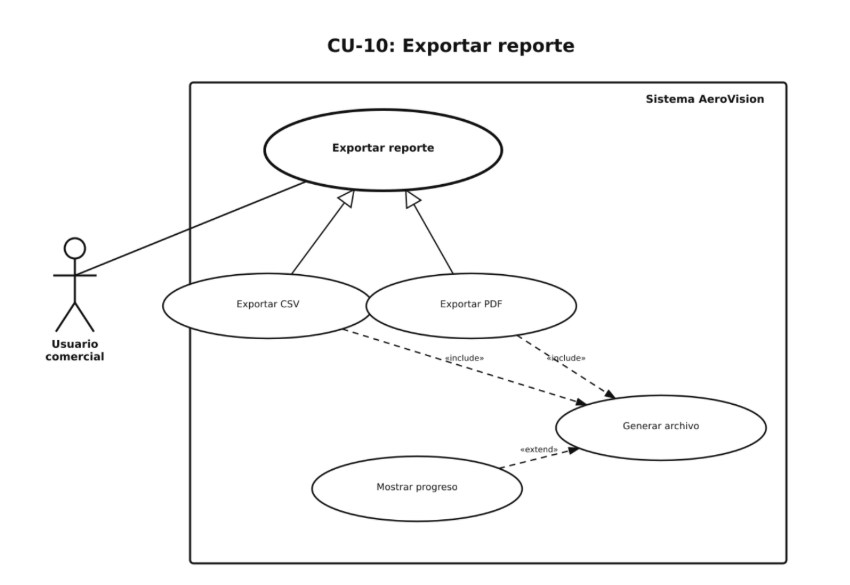
\includegraphics[width=0.85\columnwidth]{CasosdeUSO/10.png}
\caption{CU-10: Exportar reporte}
\label{fig:cu10}
\end{figure}

% ------------------------------------------------------------
\textbf{CU-11: Procesar videos multicámara}

\textbf{Actor principal:} Usuario administrador \\
\textbf{Requerimiento:} RF-06

\textbf{Historia de usuario:} Como usuario administrador, quiero que el sistema procese los videos de varias cámaras y siga a las personas de forma anónima entre ellas, para obtener trayectorias completas sin identificar a nadie.

\textbf{Precondiciones:} Videos y configuración de cámaras disponibles.

\textbf{Flujo principal:}
\begin{enumerate}
    \item El usuario inicia el procesamiento de los videos.
    \item El sistema abre una sesión de análisis con su configuración y
    el manifiesto de los modelos.
    \item El sistema detecta y sigue a las personas en cada cámara.
    \item El sistema asocia a la misma persona entre cámaras.
    \item El sistema ubica cada posición en el plano.
    \item El sistema reconcilia las identidades y registra las
    trayectorias anónimas.
\end{enumerate}

\textbf{Flujos alternativos:} Si una cámara no está calibrada, la
trayectoria se registra sin coordenadas en el plano. Si el usuario
interrumpe el procesamiento, se conserva y reconcilia lo procesado hasta
ese momento.

\textbf{Postcondiciones:} Trayectorias disponibles para el mapa y los insights.

\FloatBarrier

\begin{figure}[H]
\centering
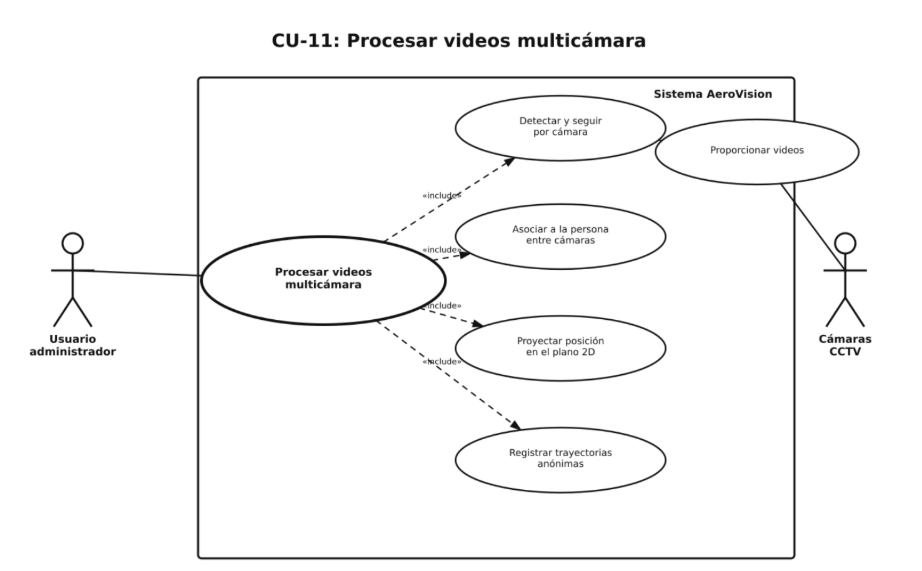
\includegraphics[width=0.85\columnwidth]{CasosdeUSO/11.png}
\caption{CU-11: Procesar videos multicámara}
\label{fig:cu11}
\end{figure}
% ============================================================
\subsection{Requerimientos Funcionales y No Funcionales}

\begin{table}[!ht]
\caption{Requisitos Funcionales y No Funcionales}
\label{tab:requisitos}
\centering
\footnotesize
\setlength{\tabcolsep}{5pt}
\renewcommand{\arraystretch}{0.9}
\begin{tabular}{p{1cm}p{2.2cm}p{6cm}p{7.5cm}}
\hline
\textbf{ID} & \textbf{Tipo} & \textbf{Requisito} & \textbf{Criterio de aceptación / Verificación} \\
\hline
RF-01 & Funcional & Autenticación y control de acceso por roles & Solo usuarios autenticados acceden; el usuario comercial consulta y el usuario administrador además configura y procesa \\
RF-02 & Funcional & Monitoreo en vivo sobre el mapa 2D & Plano con personas anónimas, estado, zona actual, trayectorias y video de las cámaras asignadas \\
RF-03 & Funcional & Personalización del mapa, cámaras y zonas & Ubicar cámaras con su cobertura y dibujar zonas con nombre, tipo y color; crear, modificar y eliminar con cambios persistentes \\
RF-04 & Funcional & Análisis histórico del movimiento & Reproducción temporal, mapa de calor y flujos entre zonas para un periodo filtrado \\
RF-05 & Funcional & Insights comerciales segmentados por zona & Visitas, pass-by, permanencia, captación y densidad por zona y periodo; exportables \\
RF-06 & Funcional & Seguimiento multicámara anónimo de personas & Detectar y seguir personas, asociarlas entre cámaras sin reconocimiento facial, asignar identificador anónimo y registrar trayectorias \\
RNF-01 & No Funcional & Seguridad & Contraseñas almacenadas con hash, conexión segura, autorización por rol verificada en el backend y límite de peticiones por IP \\
RNF-02 & No Funcional & Privacidad y normativa & Sin rostros, recortes, embeddings ni video almacenados; fichas de apariencia eliminadas al salir la persona; solo identificadores seudónimos de sesión; cumplimiento de la Ley N.\textdegree~29733 \\
RNF-03 & No Funcional & Integridad de datos & Rechazo de cambios simultáneos conflictivos, de geometrías inválidas y de filas que violen las restricciones del esquema \\
RNF-04 & No Funcional & Rendimiento & Consultas y actualización del mapa en tiempos aceptables para la operación \\
RNF-05 & No Funcional & Fluidez de visualización & Animación continua y respuesta inmediata a la interacción \\
RNF-06 & No Funcional & Disponibilidad & Verificación de estado y recuperación automática ante fallos \\
RNF-07 & No Funcional & Portabilidad & Despliegue en contenedores; plano local sin servicios externos \\
RNF-08 & No Funcional & Usabilidad & Confirmación antes de borrar; interfaz aprendible sin capacitación extensa \\
RNF-09 & No Funcional & Mantenibilidad & API versionada, migraciones de base de datos versionadas y pruebas automatizadas \\
RNF-10 & No Funcional & Compatibilidad & Funcionamiento en navegadores modernos; cámara solo con conexión segura \\
RNF-11 & No Funcional & Precisión del seguimiento & Identidades consistentes dentro de cada cámara y entre cámaras, validadas con videos etiquetados \\
RNF-12 & No Funcional & Rendimiento del procesamiento de video & Procesamiento de varias cámaras simultáneas al ritmo del video \\
RNF-13 & No Funcional & Reproducibilidad & Pesos, configuración y versiones de dependencias registrados con huella SHA-256 en cada sesión de análisis \\
\hline
\end{tabular}
\end{table}

\FloatBarrier

%% ============================================================
%% VI. Metodología
%% ============================================================

\section{Metodología}

AeroVision propone una metodología de tres partes encadenadas para
transformar el video CCTV en trayectorias espaciales anónimas y,
posteriormente, convertir esas trayectorias en indicadores operativos y
comerciales. En la primera parte se construye y estabiliza el seguimiento
local de personas dentro de cada cámara. En la segunda, los tracklets de
todas las cámaras se asocian mediante una galería global compartida,
reciben un identificador anónimo y se proyectan sobre un plano 2D común
mediante homografía. En la tercera, las trayectorias históricas se
procesan para detectar zonas de concentración, rutas frecuentes, flujos
entre zonas y métricas de comportamiento.

El flujo metodológico general es:

\begin{equation}
\begin{aligned}
\text{CCTV}
&\rightarrow \text{Tracking local}
\rightarrow \text{Re-ID multicámara} \\
&\rightarrow \text{Mapeo 2D}
\rightarrow \text{Histórico} \\
&\rightarrow \text{Insights}.
\end{aligned}
\end{equation}

El núcleo metodológico está compuesto por YOLO26m para la detección de
personas; un seguidor local híbrido basado en movimiento, IoU, escala,
apariencia corporal (histogramas de color y ResNet18) y memoria visual;
el codificador YOLO26s-ReID con una galería global compartida para la
asociación entre cámaras; homografía para la proyección espacial; un
modelo CLIP local, opcional, para la estimación agregada de género;
PostGIS para el almacenamiento espacial; y Vue.js para la visualización.

Ningún modelo se entrena dentro del proyecto: todos los pesos son
preentrenados, se cargan desde disco sin descargas ni telemetría, y cada
ejecución exporta un manifiesto con la huella SHA-256 de los pesos, de la
configuración y del propio notebook, junto con las versiones de las
dependencias (PyTorch, Ultralytics, OpenCV, ONNX Runtime, entre otras).
Los umbrales del seguidor y de la asociación se guardan en dos archivos
versionados: uno para la detección y el seguimiento local, y otro para
el registro de cámaras y la asociación multicámara.

%% ============================================================
\subsection{Parte I: Construcción del seguimiento local}

La primera parte mantiene una identidad local estable mientras una
persona permanece en el campo de visión de una cámara. El seguimiento
debe conservar el identificador ante desplazamientos, cambios de
orientación, cruces entre personas, oclusiones parciales y pérdidas
breves de detección.

Cada cámara ejecuta una instancia independiente del seguidor y procesa
sus cuadros en orden temporal estrictamente creciente, sin omitir
ninguno, de modo que cada observación utiliza como contexto el estado
construido en los cuadros anteriores. El detector y el extractor de
apariencia se cargan una sola vez y se comparten entre cámaras. El
seguidor también se actualiza en los cuadros sin detecciones, para que
el tiempo de ausencia de cada track siga avanzando.

%% ---------------------------------------------------------
\subsubsection{Detección de personas}

Cada cuadro se procesa con YOLO26m restringido a la clase
\textit{person}, con una entrada de 640 píxeles. Cada detección se
representa como:

\begin{equation}
d_i = (x_1,y_1,x_2,y_2,c_i),
\end{equation}

donde $c_i$ es la confianza del detector. Para aprovechar la GPU, el
detector procesa en un mismo lote un cuadro de cada cámara
correspondiente al mismo instante, sin mezclar nunca cuadros de instantes
distintos. Se utiliza precisión completa (FP32), porque la media
precisión alteraba levemente las confianzas y, con ello, decisiones del
seguidor cercanas a los umbrales.

Las detecciones se aceptan desde una confianza de 0.30, que coincide con
el umbral de visualización, de modo que todo lo que se sigue también se
dibuja. Las detecciones de confianza baja se conservan, pero solo pueden
prolongar un track existente; nunca crean una identidad nueva. Este
criterio es deliberado: elevar solo el umbral del detector no reduce los
identificadores espurios, porque son precisamente las detecciones débiles
las que sostienen un track durante una oclusión. La persistencia de la
identidad es, por tanto, responsabilidad del seguidor.

%% ---------------------------------------------------------
\subsubsection{Limpieza de detecciones}

Antes de la asociación se descartan las cajas contenidas en al menos un
92\,\% dentro de otra caja de la misma escena y las cajas con una altura
menor a 40 píxeles, demasiado pequeñas para representar a una persona
con detalle suficiente para su apariencia y su re-identificación.

Además, se delimita el área útil de cada cámara, estimada a partir de
varios cuadros del video, de modo que las bandas negras producidas por
el recorte no se consideren como borde de la escena. Esta área se usa
luego para reconocer las cajas cortadas por el borde inferior.

Este procedimiento reduce los identificadores espurios producidos por
detecciones duplicadas, intermitentes o de personas muy lejanas.

%% ---------------------------------------------------------
\subsubsection{Predicción de movimiento y continuidad espacial}

Cada track conserva su caja más reciente y su velocidad en la imagen,
que se actualiza de forma amortiguada para no reaccionar en exceso a una
detección ruidosa. Con esta información se predice la caja esperada
$B_p$ en el cuadro siguiente.

La compatibilidad espacial entre una detección y un track considera la
distancia entre sus centros, la superposición de las cajas y el cambio
de escala. La superposición se mide con Intersection over Union:

\begin{equation}
IoU(B_p,B_d)=
\frac{|B_p \cap B_d|}
{|B_p \cup B_d|},
\end{equation}

donde $B_d$ es la caja de la detección actual. El cambio de escala se
mide en escala logarítmica sobre el ancho $w$ y el alto $h$:

\begin{equation}
\Delta s=
\frac{1}{2}
\left(
\left|\ln\frac{w_d}{w_p}\right|
+
\left|\ln\frac{h_d}{h_p}\right|
\right).
\end{equation}

Esta medida tolera que una persona que se acerca o se aleja de la cámara
cambie de tamaño gradualmente, sin interpretar ese cambio como un cambio
de identidad.

%% ---------------------------------------------------------
\subsubsection{Extracción de apariencia sin reconocimiento facial}

Cuando la información espacial no basta para diferenciar a personas
cercanas, el seguidor incorpora la apariencia corporal, sin utilizar
reconocimiento facial. El recorte de cada detección se divide en tres
regiones: cabeza, torso y piernas, con pesos de 0.20, 0.52 y 0.28,
respectivamente. De cada región visible se obtienen histogramas de color
en los espacios HSV (tono y saturación, y brillo) y Lab (componentes
cromáticas), normalizados para que su comparación no dependa del tamaño
del recorte.

Las partes de una región cubiertas por la caja de otra persona se
enmascaran antes de calcular los histogramas, para no mezclar la
apariencia de dos identidades durante un cruce.

Además, una ResNet18 preentrenada en ImageNet, sin su capa de
clasificación, se utiliza únicamente como extractor de características
profundas. El recorte se redimensiona a $64\times128$ píxeles, el mapa
de características se promedia en cuatro franjas horizontales y el
resultado (2\,048 valores) se normaliza con la norma L2, lo que conserva
la disposición vertical de la vestimenta. La representación de
apariencia es:

\begin{equation}
A=[A_{\text{color}},A_{\text{deep}}].
\end{equation}

La similitud de apariencia combina ambas componentes mediante una mezcla
calibrada:

\begin{equation}
S_{\text{app}}=
\operatorname{clip}\!\Big(
\gamma\big[(1-\omega)\,S_{\text{color}}+\omega\,S_{\text{deep}}\big]
+\beta,\ 0,\ 1
\Big),
\end{equation}

donde $\omega=0.20$ es el peso de la componente profunda, y $\gamma=1.123$
y $\beta=-0.075$ son coeficientes de calibración que ajustan la escala de
la similitud a la de los demás términos de la asociación. Si alguna de
las dos observaciones no tiene componente profunda, se usa solo la
similitud de color.

%% ---------------------------------------------------------
\subsubsection{Cálculo selectivo de la apariencia}

La apariencia no se calcula para cada persona en cada cuadro. Los
histogramas por región y la ResNet18 solo se evalúan cuando pueden
cambiar una decisión:

\begin{itemize}
    \item cuando una detección está cerca de un track, pero con poca
    superposición;
    \item cuando dos tracks o dos detecciones compiten entre sí;
    \item cuando se intenta recuperar un track perdido;
    \item cuando aparece una persona nueva o tentativa;
    \item y en el refresco periódico de la galería de cada track, cada
    cinco cuadros.
\end{itemize}

Si el movimiento, la superposición y la escala bastan para decidir, la
apariencia se omite. Aun cuando se calcula solo para una parte de las
detecciones, esta estrategia se diseñó para producir las mismas
decisiones que el cálculo en todos los cuadros, lo que se verifica
comparando ambas configuraciones sobre los mismos videos.

%% ---------------------------------------------------------
\subsubsection{Memoria visual multivista}

Cada track conserva una galería acotada de hasta 24 vistas fiables
obtenidas durante su recorrido, que puede incluir vistas frontales,
laterales y posteriores. Una nueva observación $q$ se compara con la
galería $G_i$ del track mediante:

\begin{equation}
S_{\text{app}}(q,G_i)=
\max_{g \in G_i}
\operatorname{sim}(q,g).
\end{equation}

Así, la decisión no depende solo de la apariencia del cuadro anterior. La
comparación se calcula de forma vectorizada para todos los pares de
tracks y detecciones del cuadro. La galería solo se actualiza con vistas
fiables: detecciones con confianza de al menos 0.55, con un solape menor
a 0.25 con otras personas y con evidencia de color suficiente.

%% ---------------------------------------------------------
\subsubsection{Estados de un track}

Cada identidad local atraviesa tres estados:

\begin{itemize}
    \item \textbf{Tentativo:} la detección aún no reúne evidencia
    suficiente y no se publica ningún identificador.
    \item \textbf{Confirmado:} el track recibe un \textit{local\_id}
    estable y participa en la asociación principal.
    \item \textbf{Perdido:} el track dejó de detectarse, pero conserva su
    última caja, velocidad, escala y galería durante una edad máxima;
    pasado ese tiempo se elimina.
\end{itemize}

Cuando un track se recupera tras una pérdida o se asocia durante un
cruce, se marca como \textit{en riesgo} en ese cuadro, lo que permite
avisar a la etapa multicámara.

%% ---------------------------------------------------------
\subsubsection{Asociación en cascada}

Para cada cuadro, la asociación entre tracks y detecciones se resuelve en
cinco etapas ordenadas:

\begin{enumerate}
    \item \textbf{Asociación principal.} Las detecciones con confianza de
    al menos 0.35 se comparan con los tracks observados en el cuadro
    anterior mediante la puntuación:
    \begin{equation}
    \begin{aligned}
    S_{ij} ={}&
    w_mS_{\text{mov}}
    +w_oS_{\text{IoU}} \\
    &+w_sS_{\text{escala}}
    +w_aS_{\text{app}},
    \end{aligned}
    \end{equation}
    donde $w_m$, $w_o$, $w_s$ y $w_a$ son los pesos de cada componente.

    \item \textbf{Segunda etapa.} Siguiendo la lógica de ByteTrack, una
    detección de confianza baja solo puede prolongar un track activo que
    haya quedado libre y con el que muestre un movimiento, una
    superposición y una escala muy coherentes (umbrales de movimiento e
    IoU de 0.55 y 0.12).

    \item \textbf{Recuperación.} Las detecciones fiables que siguen sin
    asignar se comparan con los tracks perdidos recientemente, usando su
    galería de apariencia, la posición esperada y la escala.

    \item \textbf{Actualización.} Los tracks asignados actualizan su
    caja, su velocidad amortiguada y, si la vista es fiable, su galería.

    \item \textbf{Creación de tracks.} Las detecciones restantes solo
    generan un track nuevo tras confirmarse al menos tres veces, con
    confianza de al menos 0.60, dentro de una ventana de cinco cuadros,
    de modo que no se publican identificadores efímeros.
\end{enumerate}

En cada etapa, la asignación uno a uno se resuelve con el algoritmo
Hungarian sobre una matriz de costos ampliada con columnas ficticias. Si
$C\in\mathbb{R}^{n\times m}$ es la matriz de costos y $\tau$ el costo
máximo aceptado, se construye:

\begin{equation}
\tilde{C}=
\big[\,C' \;\big|\; (\tau+\epsilon)\,\mathbf{1}_{n\times n}\,\big],
\qquad
C'_{ij}=
\begin{cases}
C_{ij}, & C_{ij}\le\tau,\\
\infty, & C_{ij}>\tau.
\end{cases}
\end{equation}

Asignar una fila a una columna ficticia equivale a dejar ese track sin
detección. De esta forma, un track puede quedar sin asignar sin quitarle
la detección a otro par válido, y ninguna detección se asocia a dos
tracks a la vez.

Como los videos pueden tener distintas tasas de cuadros, el tiempo máximo
de pérdida de un track y la ventana de confirmación se definen para una
tasa de referencia $f_{\text{ref}}=15$~FPS y se escalan con la tasa real
$f_c$ de cada cámara:

\begin{equation}
N_c = \max\!\left(1,\ \operatorname{round}\!\left(N_{\text{ref}}\,\frac{f_c}{f_{\text{ref}}}\right)\right).
\end{equation}

La ventana de confirmación escalada nunca es menor que el número de
confirmaciones exigidas.

%% ---------------------------------------------------------
\subsubsection{Manejo de cruces y oclusiones}

Durante un cruce o una superposición, cada identidad conserva su estado
previo y la actualización de su apariencia se restringe, ya que las
regiones cubiertas se enmascaran y las vistas muy solapadas no ingresan
a la galería.

Cuando una persona deja de detectarse, su track no se elimina de
inmediato: permanece en estado perdido durante un máximo de 120 cuadros
(8~s a 15~FPS). Esto permite distinguir una oclusión breve de una salida
definitiva del campo de visión. El seguidor también informa a la etapa
multicámara cuando detecta un cruce o una recuperación, para que la
identidad afectada se verifique de inmediato.

%% ---------------------------------------------------------
\subsubsection{Recuperación de identidades}

Tras la asociación principal, las detecciones fiables no asignadas se
comparan con los tracks perdidos considerando coherencia de apariencia
(umbral de color de 0.72), posición esperada (umbral de distancia de
0.95), dirección, escala y movimiento previo. Si la evidencia es
suficiente, se recupera el mismo \textit{local\_id}; si no, la detección
sigue el proceso de confirmación de un track nuevo.

%% ---------------------------------------------------------
\subsubsection{Parámetros del seguimiento local}

El Cuadro~\ref{tab:tracker_params} resume los parámetros configurables
del seguidor y los valores utilizados en el piloto. Sus valores se
definen en un archivo de configuración versionado junto con los pesos de
los modelos y se ajustaron sobre los videos del piloto, por lo que deben
revisarse al incorporar cámaras nuevas.

\begin{table}[H]
\caption{Parámetros del seguimiento local}
\label{tab:tracker_params}
\centering
\footnotesize
\begin{tabular}{p{0.30\columnwidth}p{0.14\columnwidth}p{0.48\columnwidth}}
\hline
\textbf{Parámetro} & \textbf{Valor} & \textbf{Función} \\
\hline
Confianza mínima de detección & 0.30 & Detecciones que el seguidor puede usar. \\
IoU de supresión del detector & 0.50 & Fusión de cajas redundantes en YOLO26m. \\
Confianza de asociación & 0.35 & Detecciones admitidas en la asociación principal. \\
Confianza para nuevo track & 0.60 & Detecciones que pueden iniciar una identidad. \\
Confirmaciones y ventana & 3 en 5 cuadros & Detecciones necesarias para publicar un track. \\
Edad máxima & 120 cuadros & Tiempo que un track perdido puede recuperarse. \\
Umbrales de movimiento e IoU & 0.55 / 0.12 & Coherencia exigida en la segunda etapa. \\
Umbrales de color y distancia & 0.72 / 0.95 & Coherencia exigida en la recuperación. \\
Tamaño de galería & 24 vistas & Vistas fiables conservadas por track. \\
Peso profundo y calibración & 0.20; 1.123 / $-$0.075 & Mezcla entre color y ResNet18. \\
Intervalo de apariencia & 5 cuadros & Frecuencia de refresco de la galería. \\
Altura mínima & 40 px & Tamaño mínimo de una persona válida. \\
FPS de referencia & 15 & Base para escalar edad y ventana. \\
\hline
\end{tabular}
\end{table}

%% ---------------------------------------------------------
\subsubsection{Salida del seguimiento local}

La salida de cada observación es:

\begin{equation}
\begin{aligned}
(&camera\_id,\ frame,\ timestamp,\ local\_id,\\
&bbox,\ confidence,\ appearance,\ riesgo).
\end{aligned}
\end{equation}

El \textit{local\_id} solo es válido dentro de la cámara que lo creó. La
asociación entre cámaras se realiza en la Parte II.

%% ============================================================
\subsection{Parte II: Procesamiento multicámara y mapeo 2D}

La segunda parte comienza con el seguimiento local estabilizado. Cada
cámara sigue trabajando de manera independiente, pero sus tracklets se
comparan contra una misma memoria global para decidir qué observaciones
pertenecen a la misma persona, y sus posiciones se transforman a un
sistema espacial común correspondiente al plano físico del aeropuerto.
El resultado es un identificador anónimo global para cada persona.

%% ---------------------------------------------------------
\subsubsection{Registro técnico de cámaras}

Cada cámara dispone de una configuración técnica que la relaciona con el
resto de la infraestructura (Cuadro~\ref{tab:camera_configuration}).
Además de los datos propios de cada cámara, el registro declara qué pares
de cámaras comparten campo de visión y qué transiciones entre cámaras son
físicamente posibles. El identificador de cada cámara debe coincidir con
el nombre de su video y con el registrado en la base de datos.

\begin{table}[H]
\caption{Configuración técnica de las cámaras}
\label{tab:camera_configuration}
\centering
\footnotesize
\begin{tabular}{p{0.28\columnwidth}p{0.64\columnwidth}}
\hline
\textbf{Campo} & \textbf{Uso} \\
\hline
camera\_id & Identificador interno único (por ejemplo, \texttt{cam01}). \\
stream\_uri & Origen RTSP o archivo de video. \\
fps / resolución & Configuración efectiva del stream. \\
timestamp\_offset & Corrección temporal de la cámara. \\
$H$ & Matriz de homografía (si la cámara está calibrada). \\
coverage\_polygon & Área visible sobre el plano. \\
max\_error\_m & Error máximo aceptado en los puntos de control. \\
overlaps & Pares de cámaras con campo de visión compartido. \\
transitions & Cámaras de destino posibles, con ventana $[t_{\min},t_{\max}]$ y, en modo calibrado, distancia y dirección admisibles. \\
mode & Modo de asociación: visual-temporal o calibrado. \\
\hline
\end{tabular}
\end{table}

%% ---------------------------------------------------------
\subsubsection{Sincronización temporal}

La asociación multicámara utiliza diferencias de tiempo entre
observaciones, por lo que todos los streams deben compartir una
referencia temporal. Para el cuadro $k$ de la cámara $c$, con tasa $f_c$
y desfase $\delta_c$, el tiempo común es:

\begin{equation}
t_{c,k}=\frac{k-1}{f_c}+\delta_c .
\end{equation}

Un desfase positivo retrasa la cámara. Un lector sincronizado entrega
los cuadros de todas las cámaras en el orden de este tiempo corregido,
sin omitir ninguno y agrupando los que caen en el mismo instante, dentro
de una tolerancia de 0.15~s. En cada instante se detecta, se actualiza
cada seguidor local y se entregan juntas las observaciones de todas las
cámaras a la galería compartida. Si una cámara termina antes, las demás
continúan. Finalmente, el tiempo común se convierte en una marca de
tiempo absoluta sumándole la hora de inicio de la grabación.

%% ---------------------------------------------------------
\subsubsection{Tracking independiente por cámara}

Cada stream ejecuta su propia instancia del seguidor de la Parte I. Por
ello, dos cámaras pueden usar el mismo \textit{local\_id} para personas
diferentes. La salida sigue siendo local hasta completar la asociación
multicámara.

%% ---------------------------------------------------------
\subsubsection{Calibración y homografía}

Cada cámara se calibra utilizando puntos del suelo visibles tanto en el
frame como en el plano 2D del aeropuerto.

Se utilizan al menos cuatro correspondencias no colineales:

\begin{equation}
(u_i,v_i)
\leftrightarrow
(X_i,Y_i).
\end{equation}

A partir de estas correspondencias se estima una matriz de homografía
$H$ específica para cada cámara.

Para aproximar la posición de una persona sobre el piso se utiliza el
punto inferior central de su caja:

\begin{equation}
u=\frac{x_1+x_2}{2},
\qquad
v=y_2.
\end{equation}

La transformación se calcula mediante:

\begin{equation}
\begin{bmatrix}
X'\\
Y'\\
W'
\end{bmatrix}
=
H
\begin{bmatrix}
u\\
v\\
1
\end{bmatrix}.
\end{equation}

Posteriormente se normalizan las coordenadas:

\begin{equation}
X=\frac{X'}{W'},
\qquad
Y=\frac{Y'}{W'}.
\end{equation}

De esta manera, las observaciones obtenidas desde cámaras diferentes
quedan expresadas dentro del mismo sistema de coordenadas y pueden
compararse mediante posición, distancia, velocidad y dirección.

%% ---------------------------------------------------------
\subsubsection{Validación de la calibración}

La matriz de homografía no se acepta únicamente mediante inspección
visual. Se reservan al menos dos puntos de control que no participan en
la estimación de $H$ y se calcula su error de reproyección sobre el
plano. Se rechazan además los puntos degenerados y los controles
repetidos.

Cuando el error supera el umbral establecido para la escala utilizada
(0.75~m en el piloto), la calibración se repite modificando o
incrementando los puntos de correspondencia.

%% ---------------------------------------------------------
\subsubsection{Modos de asociación}

La asociación multicámara opera en uno de dos modos, según el estado de
la calibración:

\begin{itemize}
    \item \textbf{Visual-temporal:} se utiliza cuando las cámaras aún no
    tienen homografía validada. La asociación depende de la apariencia y
    de las restricciones temporales y de conectividad, y las
    coordenadas, la velocidad y la dirección en el plano quedan vacías.
    \item \textbf{Calibrado:} exige homografías validadas y añade
    restricciones métricas de posición, velocidad y dirección sobre el
    plano.
\end{itemize}

%% ---------------------------------------------------------
\subsubsection{Construcción de tracklets}

Las observaciones de un mismo \textit{local\_id} se resumen en un
tracklet:

\begin{equation}
\begin{aligned}
T=\{&
camera\_id,\ local\_id,\\
&t_{\text{inicio}},t_{\text{fin}},\\
&(X,Y,t),v,\theta,A,o
\}.
\end{aligned}
\end{equation}

Aquí, $v$ es la velocidad estimada, $\theta$ la dirección de
desplazamiento, $A$ el conjunto de vistas de apariencia y $o$ la
orientación de cada vista (frente, espalda, costado o quieto), estimada a
partir del movimiento de los pies en la imagen.

Cada tracklet se resume en un \textbf{prototipo}, que es el promedio
normalizado de los embeddings de sus vistas:

\begin{equation}
\bar{e}_T=
\frac{\sum_{k=1}^{K} e_k}
{\left\|\sum_{k=1}^{K} e_k\right\|_2}.
\end{equation}

El tracklet es la unidad de comparación entre cámaras, lo que evita
comparar indiscriminadamente todos los cuadros individuales. Si un
\textit{local\_id} reaparece tras una ausencia de más de 2~s, el nuevo
tramo se trata como un tracklet distinto y no hereda automáticamente la
identidad anterior.

%% ---------------------------------------------------------
\subsubsection{Codificador de re-identificación}

Los embeddings $e_k$ se obtienen con YOLO26s-ReID, un codificador
preentrenado en el dataset MSMT17 que produce vectores de 512
dimensiones normalizados con la norma L2. Cada recorte se amplía con el
mismo margen que utiliza Ultralytics (factor 1.02 más 10 píxeles
alrededor de la caja), se convierte a RGB, se escala a $[0,1]$ y se
redimensiona a una entrada cuadrada de $448\times448$ píxeles antes de
la inferencia; esta resolución separó mejor a las personas que la de
$224\times224$. Las vistas se procesan en lotes de ocho.

El modelo, distribuido en formato ONNX, se convierte a PyTorch para
ejecutarse en la GPU, comprobando que sus embeddings coinciden con los
del formato original (similitud coseno de al menos 0.99999). Si la
conversión no está disponible, el codificador se ejecuta con ONNX
Runtime en la CPU, con el mismo resultado y mayor latencia.

Entre cámaras solo se utiliza este codificador. Los histogramas de color
se reservan para el seguimiento local, porque combinarlos con el
codificador no mejoró la separación entre la misma persona y personas
distintas.

%% ---------------------------------------------------------
\subsubsection{Muestreo y verificación de vistas}

El codificador no se aplica a cada cuadro. Se muestrea una vista fiable
de cada persona cada 0.4~s mientras aún no esté bien descrita, es decir,
cuando:

\begin{itemize}
    \item su tracklet tiene menos de 10 vistas;
    \item su ficha en la galería global tiene menos de 40 vistas;
    \item o aparece una orientación nueva en su tracklet.
\end{itemize}

Una vista es fiable si su detección tiene una confianza de al menos 0.55,
una altura de al menos 40 píxeles y una oclusión menor al 20\,\%. Una vez
descrita, la identidad solo se verifica cada 2~s, salvo que el seguidor
local la marque en riesgo por un cruce o una recuperación, o que exista
sospecha de cambio de persona; en esos casos se verifica de inmediato.
No se descartan vistas por orientación, ya que la robustez del
codificador proviene de promediar muchas vistas de la misma persona:
conservar solo unas pocas vistas por orientación reduce de forma marcada
la capacidad de reunir a una misma persona.

%% ---------------------------------------------------------
\subsubsection{Detección de cambio de persona}

El seguidor local puede entregar ocasionalmente el mismo
\textit{local\_id} a otra persona, por ejemplo en puertas o detrás de
columnas. Si dos vistas consecutivas quedan por debajo de una similitud
de 0.40 respecto al prototipo de su tracklet, el tracklet se corta y el
tramo siguiente se trata como una identidad nueva, que la galería vuelve
a evaluar.

%% ---------------------------------------------------------
\subsubsection{Galería global compartida}

Todas las cámaras se comparan a la vez contra una misma memoria. Cada
persona es una ficha de la galería que contiene las vistas de todos sus
tracklets en todas las cámaras, con su orientación; el lugar y el
momento en que se vio por última vez; y el tiempo que lleva visible.
Cuando una cámara observa a alguien, lo compara con esa ficha, que ya
incluye lo que vieron las demás cámaras. Así, una persona vista de
espaldas en una cámara puede reconocerse de frente en otra.

La galería se organiza en cinco componentes con responsabilidades
separadas: el estado (tracklets, identidades internas e identificadores
públicos), la recepción de observaciones y el muestreo de vistas, el
filtrado físico, la fusión y separación de identidades, y los reportes
de auditoría.

%% ---------------------------------------------------------
\subsubsection{Grafo de conectividad entre cámaras}

La disposición física de las cámaras se representa mediante un grafo de
conectividad. Para cada cámara se definen aquellas hacia las cuales una
persona puede desplazarse y aquellas con las que comparte campo de
visión. Para cada transición $i\rightarrow j$ se establece una ventana
temporal plausible:

\begin{equation}
t_{\min}(i,j)
\leq
\Delta t
\leq
t_{\max}(i,j).
\end{equation}

Así, un tracklet que termina en una cámara solo genera candidatos en las
cámaras conectadas y dentro de una ventana temporal válida. Además, solo
se consideran candidatas las identidades vistas en los últimos 90~s.

%% ---------------------------------------------------------
\subsubsection{Restricciones físicas}

Antes de comparar apariencias, se descartan las asociaciones físicamente
imposibles. Dos identidades solo pueden fusionarse si se cumplen todas
las condiciones siguientes:

\begin{enumerate}
    \item Una identidad no puede tener dos tracklets simultáneos en la
    misma cámara.
    \item Dos cámaras solo pueden observar a la misma persona al mismo
    tiempo si están declaradas con solape.
    \item Entre segmentos consecutivos de cámaras sin solape debe existir
    la transición $i\rightarrow j$ dentro de $[t_{\min},t_{\max}]$.
    \item Una re-entrada en la misma cámara debe ocurrir dentro de una
    ventana de re-entrada de 120~s.
    \item En modo calibrado, además, la distancia entre el punto de
    salida y el de entrada, la velocidad requerida (como máximo
    4~m/s) y la dirección deben ser coherentes con el desplazamiento de
    una persona, y dos cámaras con solape deben ubicarla a menos de
    1.5~m.
\end{enumerate}

Estas restricciones reducen el espacio de búsqueda y evitan que dos
personas parecidas se fusionen solo por su apariencia.

%% ---------------------------------------------------------
\subsubsection{Similitud y criterios de fusión}

Las identidades que superan las restricciones físicas se comparan
mediante la similitud coseno entre sus fichas:

\begin{equation}
s(a,b)=\cos\!\left(\bar{e}_a,\bar{e}_b\right)\ \geq\ \tau .
\end{equation}

Para que un único tracklet parecido no encadene a personas distintas, se
exige además que el enlace promedio entre todos sus tracklets supere un
segundo umbral:

\begin{equation}
\bar{s}(a,b)=
\frac{1}{|T_a|\,|T_b|}
\sum_{t\in T_a}\sum_{u\in T_b}
\cos\!\left(\bar{e}_t,\bar{e}_u\right)
\ \geq\ \tau_{\text{avg}} .
\end{equation}

En el piloto se utilizan $\tau=0.60$ y $\tau_{\text{avg}}=0.55$. Además,
se aplican tres reglas:

\begin{itemize}
    \item \textbf{Re-entrada en una sola cámara.} Si toda la evidencia
    proviene de la misma cámara, se exige un umbral mayor
    ($\tau_{\text{cam}}=0.70$), porque con la misma iluminación y el
    mismo fondo las personas distintas se parecen más que entre cámaras.
    \item \textbf{Ausencia de ambigüedad.} Si la mejor candidata $b^{*}$ y
    otra candidata $b'$ incompatible con ella quedan demasiado cerca, la
    decisión se posterga:
    \begin{equation}
    s(a,b^{*})-s(a,b')\ \geq\ m, \qquad m=0.05 .
    \end{equation}
    \item \textbf{Preferencia mutua.} La fusión solo se realiza si la
    ficha destino también prefiere a la identidad que la propone.
\end{itemize}

Cuando se fusionan, las dos identidades se unen en la más antigua, que
conserva su identificador. Si una fusión posterior deja de ser
físicamente posible, el tracklet en conflicto se separa. Las fusiones y
separaciones se registran en una bitácora de enlaces con su puntuación,
entendida como una similitud y no como una probabilidad de acierto.

Los umbrales de este apartado se calibraron con tracklets etiquetados
manualmente sobre los videos del piloto (Cuadro~\ref{tab:assoc_params}).

\begin{table}[H]
\caption{Parámetros de la asociación multicámara}
\label{tab:assoc_params}
\centering
\footnotesize
\begin{tabular}{p{0.36\columnwidth}p{0.12\columnwidth}p{0.44\columnwidth}}
\hline
\textbf{Parámetro} & \textbf{Valor} & \textbf{Función} \\
\hline
Intervalo de muestreo & 0.4~s & Frecuencia de vistas para el codificador. \\
Vistas por tracklet / identidad & 10 / 40 & Objetivo para considerar descrita a una persona. \\
Intervalo de verificación & 2~s & Revisión de identidades ya descritas. \\
Umbral de fusión $\tau$ & 0.60 & Similitud mínima entre fichas. \\
Enlace promedio $\tau_{\text{avg}}$ & 0.55 & Evita encadenar personas distintas. \\
Umbral en una sola cámara & 0.70 & Re-entradas con igual fondo e iluminación. \\
Margen de ambigüedad $m$ & 0.05 & Posterga decisiones dudosas. \\
Corte por cambio de persona & 0.40 $\times$ 2 & Similitud y vistas seguidas para cortar. \\
Vistas mínimas (unión / nueva) & 4 / 5 & Evidencia para unirse o crear una identidad. \\
Duración mínima visible & 2~s & Requisito para una identidad nueva. \\
Ventana de candidatos & 90~s & Antigüedad máxima de una candidata. \\
Ventana de re-entrada & 120~s & Re-aparición en la misma cámara. \\
Separación entre tracklets & 2~s & Ausencia que inicia un tracklet nuevo. \\
Tolerancia de sincronía & 0.15~s & Agrupación de cuadros simultáneos. \\
\hline
\end{tabular}
\end{table}

%% ---------------------------------------------------------
\subsubsection{Identidades provisionales y pasadas breves}

Una persona nueva comienza sin identificador público:

\begin{itemize}
    \item \textbf{Se une a una identidad conocida} si, con al menos
    cuatro vistas, ya coincide con una ficha confirmada.
    \item \textbf{Recibe un identificador nuevo} solo si permaneció
    visible al menos 2~s y reunió al menos cinco vistas.
    \item \textbf{No se contabiliza} si pasó brevemente por una cámara y
    no coincide con nadie; en ese caso no se exporta ni se incluye en el
    total de personas.
\end{itemize}

Esta regla evita inflar el conteo con detecciones fugaces que no aportan
información suficiente para una identidad confiable.

%% ---------------------------------------------------------
\subsubsection{Identificador global anónimo}

Los tracklets asociados reciben un \textit{global\_id}, que es un
seudónimo técnico válido solo durante la sesión de análisis. Durante el
procesamiento se muestran identificadores consecutivos por orden de
aparición; estas decisiones en línea pueden cambiar si aparece nueva
evidencia de fusión o un conflicto.

Al finalizar, o si el usuario interrumpe el procesamiento, las
identidades se \textbf{reconcilian}: cada observación toma su tracklet
definitivo (después de los cortes por cambio de persona) y el
identificador público final, numerado de nuevo de forma consecutiva por
orden de primera aparición. Luego, cada identidad se exporta con un UUID
versión~5 derivado del identificador aleatorio de la sesión y de la
identidad reconciliada, y cada tracklet con un UUID derivado de la
sesión, la cámara y su identificador local. Los videos exportados y la
tabla de trayectorias usan siempre la identidad reconciliada.

El identificador no almacena nombre, rostro, documento de identidad ni
ningún otro dato civil del pasajero. Su única función es reconstruir una
trayectoria continua a través de las cámaras. El sistema no guarda
recortes, embeddings ni cuadros sueltos como resultado del
procesamiento.

%% ---------------------------------------------------------
\subsubsection{Expiración de identidades y descarte del video}

La galería global solo mantiene a las personas que todavía pueden
reaparecer. Cuando una identidad deja de observarse en todas las
cámaras, su ficha permanece en memoria únicamente durante la ventana de
re-entrada (120~s) y la ventana de candidatos (90~s), el tiempo
necesario para reconocerla si vuelve a entrar al campo de visión de
otra cámara. Vencidas ambas ventanas, se considera que la persona salió
de la zona cubierta y su identidad se \textbf{cierra}:

\begin{enumerate}
    \item Sus vistas, prototipos y embeddings se eliminan de la galería,
    por lo que deja de utilizarse como referencia para comparar a las
    personas que continúan dentro del aeropuerto.
    \item Se registran en la base de datos su intervalo de permanencia
    (\textit{first\_seen} y \textit{last\_seen}), sus tracklets y sus
    puntos de trayectoria, asociados solo al \textit{global\_id}
    seudónimo.
    \item Si la misma persona regresa más tarde, recibe un identificador
    nuevo, ya que no queda ninguna información de apariencia con la cual
    reconocerla.
\end{enumerate}

Este cierre tiene dos efectos. Por un lado, evita conservar la identidad
visual de una persona más allá de su recorrido observado. Por otro,
mantiene acotada la galería, lo que reduce el costo de cada comparación
y el riesgo de fusionar a una persona nueva con alguien que ya se fue.

De igual forma, el video no se almacena. Cada cuadro se procesa en
memoria y se descarta después de extraer sus detecciones; tampoco se
guardan recortes ni cuadros sueltos. Al finalizar la sesión, lo único
que persiste es la base de datos con las trayectorias seudónimas, los
eventos y las métricas agregadas.

%% ---------------------------------------------------------
\subsubsection{Estimación agregada de género (opcional)}

Como atributo demográfico aproximado, en la línea de Jin et
al.~\cite{jin2024}, el prototipo incorpora un clasificador CLIP local que
estima la presentación de género a partir del cuerpo completo mediante
clasificación sin entrenamiento adicional (\textit{zero-shot}), con dos
descripciones textuales de referencia. No utiliza el rostro como entrada
específica ni estima la edad.

Para limitar errores, solo se evalúan cajas grandes y fiables (altura de
al menos 96 píxeles y confianza de detección de al menos 0.65), una vez
cada 0.6~s y con un máximo de 12 votos por tracklet. Cada voto se pondera
por su confianza, y una etiqueta se publica solo si reúne al menos cinco
votos, con una confianza de al menos 0.72 y un margen de al menos 0.18
frente a la alternativa. Después de la re-identificación, los votos se
consolidan de nuevo por \textit{global\_id}; si no hay evidencia
suficiente, la identidad queda como ``sin determinar''.

Este resultado es una estimación visual: no se usa como identificación
ni como base única de decisiones, se reporta solo de forma agregada en
los insights y su precisión debe medirse de forma desagregada antes del
despliegue.

%% ---------------------------------------------------------
\subsubsection{Configuración del mapa y zonas}

El plano 2D utiliza un único sistema de coordenadas para todas las
cámaras. Sobre este plano se almacenan polígonos de cobertura de cámara
y polígonos semánticos correspondientes a zonas operativas y
comerciales.

Para cada establecimiento comercial se diferencian dos geometrías:

\begin{itemize}
\item \textbf{INTERIOR}: área correspondiente al ingreso real al
establecimiento.

\item \textbf{FRONTAGE}: franja situada frente al establecimiento y
utilizada para medir exposición o \textit{pass-by}.
\end{itemize}

Además de estas, se admiten zonas de tipo pasillo, entrada, check-in,
seguridad, puerta, cola y otras. La pertenencia de una posición $(X,Y)$
a cada polígono se determina mediante una operación
\textit{point-in-polygon} que incluye los bordes; si una posición cae en
varias zonas, se prioriza la zona INTERIOR y, entre las demás, la de
menor área.

Esta diferenciación permite separar a las personas que pasan frente al
establecimiento de aquellas que efectivamente ingresan.

%% ---------------------------------------------------------
\subsubsection{Arquitectura de ejecución}

El procesamiento de visión computacional se implementa mediante un
servicio Python desplegado dentro de Docker. Este componente ejecuta
YOLO26m, ResNet18, el seguidor local, YOLO26s-ReID, el clasificador CLIP
opcional, la homografía y la asociación multicámara. Utiliza la GPU
cuando está disponible y recurre a la CPU en caso contrario.

El backend utiliza Go para la API y la lógica de negocio.
PostgreSQL/PostGIS almacena las geometrías, posiciones, trayectorias y
eventos espaciales. Finalmente, Vue.js constituye la capa de
visualización.

El flujo de implementación es:

\begin{equation}
\begin{aligned}
\text{CCTV}
&\rightarrow \text{Python}\\
&\rightarrow \text{PostGIS}\\
&\rightarrow \text{Go}\\
&\rightarrow \text{Vue.js}.
\end{aligned}
\end{equation}

La comunicación entre el servicio de visión y la base de datos utiliza
datos estructurados (la tabla \textit{trajectory\_points} y sus tablas
asociadas), evitando utilizar imágenes como contrato principal entre los
componentes. El backend solo lee y agrega esos datos, y el navegador
nunca accede directamente a la base de datos.

%% ---------------------------------------------------------
\subsubsection{Salida estructurada de la Parte II}

La salida de la Parte II es la tabla \textit{trajectory\_points}, donde
cada fila indica dónde estuvo un \textit{global\_id} en un instante:

\begin{equation}
\begin{aligned}
\{&
global\_id,\ timestamp,\ camera\_id,\ local\_id,\\
&tracklet\_id,\ x,\ y,\ geom,\ zone\_id,\\
&speed\_mps,\ direction\_deg,\ confidence
\}.
\end{aligned}
\end{equation}

Los campos \textit{camera\_id}, \textit{local\_id} y
\textit{tracklet\_id} se conservan para trazabilidad, aunque no se
muestran en los dashboards comerciales. El campo \textit{confidence} es
la confianza de YOLO26m para esa detección. La velocidad (en m/s) y la
dirección (en grados, en $[0,360)$ respecto del eje $X$ del plano) se
calculan sobre una ventana de 1~s del tracklet. Las coordenadas, la
velocidad y la dirección quedan vacías cuando la cámara no está
calibrada o cuando los pies de la persona no son visibles, por ejemplo
si la caja está cortada por el borde inferior. El campo \textit{zone\_id}
se completa al asignar las zonas, y como las cámaras con solape pueden
observar a la misma persona a la vez, la consolidación de filas
simultáneas se realiza en la Parte III.

Junto con esta tabla se registran, para cada sesión, las identidades
con su estimación de género consolidada y el manifiesto de
reproducibilidad. Los videos anotados con los identificadores solo se
generan de forma opcional durante el piloto, para la validación visual
del seguimiento, y no forman parte de la operación ni se conservan.

%% ============================================================
\subsection{Parte III: Procesamiento histórico y generación de insights}

La tercera parte utiliza únicamente los datos estructurados generados
durante la Parte II. De esta manera, los análisis históricos pueden
realizarse sin volver a ejecutar los modelos de visión sobre el video
crudo.

El objetivo es transformar posiciones, zonas y eventos en información
que permita analizar concentración, movilidad, permanencia y
comportamiento espacial de los pasajeros.

%% ---------------------------------------------------------
\subsubsection{Motor de eventos espaciales}

Cada cambio de posición y cada transición entre polígonos se transforma
en un evento mediante reglas operativas definidas previamente
(Cuadro~\ref{tab:spatial_events}). Los eventos se almacenan en la tabla
\textit{spatial\_events}, con su instante de inicio, su instante de fin
cuando corresponde y su confianza.

\begin{table}[H]
\caption{Eventos espaciales de AeroVision}
\label{tab:spatial_events}
\centering
\footnotesize
\begin{tabular}{p{0.21\columnwidth}p{0.71\columnwidth}}
\hline
\textbf{Evento} & \textbf{Regla operativa} \\
\hline
EXPOSURE & Cruce por la zona FRONTAGE del establecimiento. \\
ENTER & Transición desde el exterior o FRONTAGE hacia INTERIOR. \\
DWELL & Permanencia dentro de INTERIOR durante un tiempo mínimo. \\
EXIT & Transición desde INTERIOR hacia el exterior. \\
RETURN & Nuevo ENTER después de un EXIT y un intervalo mínimo. \\
QUEUE & Permanencia en una zona de cola con velocidad reducida. \\
\hline
\end{tabular}
\end{table}

Estos eventos constituyen la base para calcular las métricas operativas
y comerciales.

%% ---------------------------------------------------------
\subsubsection{Consolidación histórica}

Los registros generados durante la operación se ordenan por
\textit{global\_id} y marca de tiempo. En esta etapa se consolidan las
observaciones simultáneas de una misma persona vista por varias cámaras
en una sola posición, dando mayor peso a la cámara que la observa con
mayor tamaño aparente; se eliminan duplicados y se corrigen saltos
espaciales físicamente inconsistentes.

A partir de los registros se generan dos representaciones
complementarias. La trayectoria espacial se expresa como:

\begin{equation}
\begin{aligned}
R_s=[
&(X_1,Y_1,t_1),\\
&\ldots,(X_n,Y_n,t_n)].
\end{aligned}
\end{equation}

La trayectoria semántica corresponde a la secuencia ordenada de zonas:

\begin{equation}
R_z=[Z_1,Z_2,\ldots,Z_m].
\end{equation}

Un recorrido puede representarse, por ejemplo, como:

\begin{equation}
\begin{aligned}
\text{Entrada}
&\rightarrow \text{Check-in}\\
&\rightarrow \text{Seguridad}\\
&\rightarrow \text{Tienda}\\
&\rightarrow \text{Puerta}.
\end{aligned}
\end{equation}

%% ---------------------------------------------------------
\subsubsection{Hotspots mediante KDE}

Para representar la concentración espacial histórica de pasajeros se
utiliza Kernel Density Estimation (KDE):

\begin{equation}
\hat{f}(x,y)
=
\frac{1}{Nh^2}
\sum_{i=1}^{N}
K
\left(
\frac{x-X_i}{h},
\frac{y-Y_i}{h}
\right),
\end{equation}

donde $h$ es el ancho de banda y $K$ la función kernel que distribuye
espacialmente la contribución de cada observación.

Se consideran dos interpretaciones del mapa de calor. El mapa de
ocupación pondera el tiempo de permanencia, mientras que el mapa de
visitantes únicos reduce el peso de una misma persona que permanece
durante muchos cuadros en una posición.

%% ---------------------------------------------------------
\subsubsection{Rutas frecuentes mediante PrefixSpan}

La trayectoria semántica de cada \textit{global\_id} es una secuencia
ordenada de zonas. Antes de aplicar PrefixSpan, las repeticiones
consecutivas de una misma zona se comprimen para que la tasa de cuadros
no modifique artificialmente los patrones.

PrefixSpan identifica las subsecuencias que aparecen repetidamente en los
recorridos. Cada patrón almacena la secuencia, su frecuencia y el
porcentaje de trayectorias en que aparece.

%% ---------------------------------------------------------
\subsubsection{Grafo origen-destino}

Las zonas se representan además mediante un grafo dirigido:

\begin{equation}
G=(V,E),
\end{equation}

donde $V$ es el conjunto de zonas y $E$ el de transiciones observadas. El
peso de una arista es:

\begin{equation}
w(Z_i,Z_j)
=
\big|\{global\_id:\ Z_i\rightarrow Z_j\}\big|,
\end{equation}

es decir, la cantidad de pasajeros únicos que se desplazaron de $Z_i$ a
$Z_j$. Esta representación permite identificar los principales flujos
origen-destino del aeropuerto.

%% ---------------------------------------------------------
\subsubsection{Tiempo de permanencia}

El tiempo de permanencia en una zona se obtiene a partir de los eventos
de entrada y salida:

\begin{equation}
DwellTime =
t_{\text{EXIT}}
-
t_{\text{ENTER}}.
\end{equation}

%% ---------------------------------------------------------
\subsubsection{Visitas y exposición}

Las visitas a una zona comercial son el número de \textit{global\_id}
únicos que generan un evento ENTER:

\begin{equation}
Visits(z)=
\big|\{global\_id:\ ENTER(z)\}\big|.
\end{equation}

La exposición es la cantidad de pasajeros únicos que atraviesan la zona
FRONTAGE:

\begin{equation}
Exposure(z)=
\big|\{global\_id:\ EXPOSURE(z)\}\big|.
\end{equation}

%% ---------------------------------------------------------
\subsubsection{Tasa de captación}

La tasa de captación es la proporción de pasajeros expuestos a un
establecimiento que posteriormente ingresan:

\begin{equation}
CaptureRate(z)=
\frac{Visits(z)}
{Exposure(z)}
\times100.
\end{equation}

Este indicador se interpreta únicamente como tasa de ingreso al local. No
es una tasa de conversión de compra, ya que el sistema no dispone de
información de ventas. Cuando no hay pasajeros expuestos, el indicador
se reporta como no disponible en lugar de cero.

%% ---------------------------------------------------------
\subsubsection{Densidad y congestión}

La densidad de una zona se define como:

\begin{equation}
Density(z,t)=
\frac{N(z,t)}
{Area(z)},
\end{equation}

donde $N(z,t)$ es la cantidad de personas activas en la zona $z$ en el
instante $t$, y $Area(z)$ se calcula directamente a partir del polígono
almacenado.

La congestión no se determina solo por el conteo. El análisis combina
cantidad de personas, densidad, duración de la concentración y velocidad
media: una zona con muchas personas y velocidad alta puede corresponder a
un flujo intenso pero continuo, mientras que una concentración
persistente con velocidad reducida es más consistente con una
aglomeración o una cola.

%% ---------------------------------------------------------
\subsubsection{Visualización de resultados}

Los resultados se presentan en una aplicación web desarrollada en
Vue.js, organizada en dos vistas. La primera es el mapa 2D del
aeropuerto, con cámaras, zonas, coberturas, trayectorias, flujos y mapas
de calor. La segunda es el módulo de insights, con visitas, exposición,
tasa de captación, tiempo de permanencia, rutas frecuentes, flujo
origen-destino, congestión y comparaciones históricas.

Los identificadores globales solo se utilizan para construir las
trayectorias internas y no se presentan como información de identidad
personal.

%% ============================================================
\subsection{Modelo de datos}

El modelo de datos se implementa en PostgreSQL con la extensión PostGIS y
se crea mediante migraciones versionadas. Todas las geometrías usan el
sistema de coordenadas local del plano, en metros, y todas las marcas de
tiempo se almacenan con zona horaria. El Cuadro~\ref{tab:bd} resume las
tablas y la Fig.~\ref{fig:bd} muestra sus relaciones.

\begin{table}[H]
\caption{Tablas del modelo de datos}
\label{tab:bd}
\centering
\footnotesize
\renewcommand{\arraystretch}{1.1}
\begin{tabular}{L{0.20\columnwidth}L{0.36\columnwidth}L{0.36\columnwidth}}
\toprule
\textbf{Tabla} & \textbf{Campos principales} & \textbf{Propósito} \\
\midrule
\multicolumn{3}{l}{\textit{Acceso}} \\
users & user\_id, name, email, password\_hash, active & Cuentas de acceso a la aplicación. \\
roles & role\_id, name & Roles ADMIN y COMMERCIAL\_USER. \\
user\_roles & user\_id, role\_id & Asignación de roles a usuarios. \\
\midrule
\multicolumn{3}{l}{\textit{Infraestructura y espacio}} \\
aero\_cameras & camera\_id, stream\_uri, fps, timestamp\_offset\_s, mode, homography, calib\_error\_m, position, coverage & Registro técnico y calibración de cada cámara. \\
camera\_links & from\_camera, to\_camera, overlap, t\_min\_s, t\_max\_s, max\_distance\_m & Grafo de solapes y transiciones entre cámaras. \\
locales & local\_id, name, category & Establecimientos comerciales. \\
aero\_zones & zone\_id, local\_id, zone\_type, geom, area\_m2 & Polígonos INTERIOR, FRONTAGE y operativos. \\
\midrule
\multicolumn{3}{l}{\textit{Seguimiento}} \\
analysis\_sessions & session\_id, recording\_start, mode, config\_sha256, status & Sesión de análisis y su configuración. \\
identities & global\_id, session\_id, public\_number, first\_seen, last\_seen, n\_cameras, gender\_estimate & Identidad seudónima reconciliada. \\
tracklets & tracklet\_id, global\_id, camera\_id, local\_id, t\_start, t\_end & Tramos por cámara de cada identidad. \\
identity\_links & session\_id, tracklet\_id, action, score & Bitácora de fusiones y separaciones. \\
trajectory\_points & global\_id, tracklet\_id, camera\_id, timestamp, x, y, geom, zone\_id, speed\_mps, direction\_deg, confidence & Posición de cada identidad en cada instante. \\
\midrule
\multicolumn{3}{l}{\textit{Analítica}} \\
spatial\_events & global\_id, zone\_id, event\_type, start\_time, end\_time, duration\_s & Eventos EXPOSURE, ENTER, DWELL, EXIT, RETURN y QUEUE. \\
\bottomrule
\end{tabular}
\end{table}

El esquema refuerza la metodología mediante restricciones: una cámara
solo puede estar en modo calibrado si tiene homografía y error de
calibración registrados; las zonas INTERIOR y FRONTAGE deben pertenecer a
un local; las coordenadas $x$ e $y$ son ambas nulas o ambas conocidas; y
la geometría del punto, el área de cada zona y la duración de cada
evento se calculan en la propia base de datos para evitar
inconsistencias. Ninguna tabla almacena imágenes, recortes ni
embeddings.

\begin{figure}[H]
    \centering
    \safeincludegraphics[width=\linewidth]{bd.png}
    \caption{Modelo entidad-relación de la base de datos de AeroVision.}
    \label{fig:bd}
\end{figure}

%% ============================================================
\subsection{Validación transversal}

La metodología se valida por componentes, cada uno con métricas
coherentes con el problema que resuelve
(Cuadro~\ref{tab:validation_methodology}).

\begin{table}[H]
\caption{Validación de los componentes}
\label{tab:validation_methodology}
\centering
\footnotesize
\begin{tabular}{p{0.30\columnwidth}p{0.62\columnwidth}}
\hline
\textbf{Componente} & \textbf{Validación} \\
\hline
Detección & Precisión, recall y mAP. \\
Seguimiento local & IDF1 y cambios de ID frente a anotaciones; fragmentación (IDs de uno o dos cuadros y duración mediana), reapariciones y cruces como auditoría sin anotaciones. \\
Re-ID multicámara & AUC de la similitud entre cámaras; precisión y recall sobre pares de tracklets etiquetados; personas contadas frente a reales. \\
Estimación de género & Proporción de identidades sin determinar y precisión desagregada frente a etiquetas manuales. \\
Homografía & Error de reproyección en puntos de control. \\
Eventos & Precisión, recall y F1. \\
Rendimiento & Cuadros por segundo por cámara y tiempo por componente. \\
Histórico & Comparación con trayectorias conocidas. \\
\hline
\end{tabular}
\end{table}

No se establece una precisión única para todo el sistema antes de contar
con suficiente \textit{ground truth}, ya que detección, seguimiento,
calibración, asociación multicámara y eventos son problemas distintos que
requieren evaluaciones independientes. Los umbrales de asociación se
calibran con tracklets etiquetados manualmente y deben volver a medirse
al incorporar cámaras nuevas o al cambiar cualquier umbral de detección,
ya que ambos niveles interactúan.

%% ============================================================
\subsection{Trazabilidad de datos}

La salida de cada parte es la entrada de la siguiente, sin generar
conjuntos de datos paralelos innecesarios. La Parte I produce:

\begin{equation}
\begin{aligned}
(&local\_id,\ bbox,\ confidence,\\
&appearance,\ timestamp).
\end{aligned}
\end{equation}

En la Parte II, esta información se transforma en tracklets con
prototipos de apariencia y, cuando hay calibración, coordenadas reales:

\begin{equation}
\begin{aligned}
(&tracklet\_id,\ X,Y,t,\ speed,\\
&direction,\ \bar{e}_T).
\end{aligned}
\end{equation}

Los prototipos $\bar{e}_T$ existen solo en memoria y se eliminan
cuando la identidad se cierra al salir la persona de la cobertura. La
salida final de la Parte II contiene:

\begin{equation}
\begin{aligned}
(&global\_id,\ tracklet\_id,\ timestamp,\ x,\ y,\\
&zone\_id,\ speed\_mps,\ direction\_deg,\ confidence).
\end{aligned}
\end{equation}

Finalmente, la Parte III transforma estos registros en información
agregada:

\begin{equation}
\begin{aligned}
\text{Trayectorias}
&\rightarrow \text{Heatmaps}\\
&\rightarrow \text{Rutas}\\
&\rightarrow \text{Flujos}\\
&\rightarrow \text{KPIs}.
\end{aligned}
\end{equation}

La metodología sigue, por tanto, un orden estricto: primero se estabiliza
la identidad de la persona dentro de cada cámara; luego los tracklets se
asocian entre cámaras mediante la galería global y se proyectan sobre el
plano 2D; y finalmente las trayectorias y eventos se consolidan para
generar análisis históricos, operativos y comerciales. Esta separación
permite que la analítica histórica trabaje sobre datos estructurados sin
volver a procesar el video crudo.

%% ============================================================
\subsection{Flujo de la metodología}

La Fig.~\ref{fig:flujo} resume el flujo general de la metodología, desde
la captura del video CCTV hasta la generación de insights: seguimiento
local por cámara, asociación multicámara con mapeo 2D, y procesamiento
histórico de las trayectorias.

\begin{figure}[H]
    \centering
    \safeincludegraphics[width=\linewidth]{flujo.png}
    \caption{Flujo de la metodología del proyecto.}
    \label{fig:flujo}
\end{figure}

%% ============================================================
%% VII. Planificación y Gestión del Proyecto
%% ============================================================

\section{Planificación y Gestión del Proyecto}

\subsection{Cronograma y tareas}

El proyecto se gestionó con la metodología \textbf{Scrum}, organizada en
sprints semanales que permitieron trabajar en ciclos cortos de entrega y
revisión continua. Como apoyo a esta planificación se elaboró un diagrama
de Gantt (Fig.~\ref{fig:gantt}), que muestra las entregas programadas de
cada integrante y facilita la identificación de plazos, dependencias y
cargas de trabajo.

\begin{figure}[H]
    \centering
    \safeincludegraphics[width=\linewidth]{GAN/diagrama.png}
    \caption{Diagrama de Gantt del proyecto.}
    \label{fig:gantt}
\end{figure}

Además, se implementó un sistema de actas semanales
(Fig.~\ref{fig:actas}) en las que se registraban las tareas asignadas a
cada integrante y su estado de cumplimiento. Las actas sirvieron como
mecanismo formal de seguimiento para evaluar el progreso individual y
colectivo, y para detectar a tiempo retrasos o desviaciones del plan.

\begin{figure}[H]
    \centering
    \safeincludegraphics[width=\linewidth]{GAN/actas.png}
    \caption{Actas de reuniones del proyecto.}
    \label{fig:actas}
\end{figure}

En conjunto, los sprints, el diagrama de Gantt y las actas semanales
fueron los instrumentos principales de control del proyecto. El
dashboard interactivo desarrollado puede consultarse en
\url{https://site-gamma-three-16.vercel.app/index.html}, y el código
fuente, incluidas las migraciones de la base de datos y el notebook del
modelo, en
\url{https://github.com/emaaa1000/proyecto-aeropuerto-2026}.

\subsection{Roles y responsabilidades}

Para distribuir adecuadamente las funciones del equipo se definieron los
roles del Cuadro~\ref{tab:roles}.

\begin{table}[H]
\centering
\caption{Roles y responsabilidades de cada integrante}
\label{tab:roles}
\renewcommand{\arraystretch}{1.3}
\begin{tabular}{L{4.2cm} L{2.6cm} L{9cm}}
\toprule
\textbf{Rol} & \textbf{Responsable} & \textbf{Responsabilidades} \\
\midrule
Líder del proyecto y Data Engineer & Neciosup & Elaboración de informes, gestión de tareas, seguimiento del avance y reporte general; preparación de los datos y configuración de los equipos de cómputo. \\
\addlinespace
Data Engineer & Fernández & Preparación de los datos para los modelos y configuración de los equipos de cómputo. \\
\addlinespace
Data Scientist & Quiliche & Implementación y desarrollo de los modelos de detección, seguimiento y re-identificación. \\
\addlinespace
Comunicación y documentación & Almeyda & Elaboración de la documentación del proyecto y de los informes en \LaTeX. \\
\addlinespace
Integración & López & Gestión del repositorio, desarrollo de los casos de uso e integración de los componentes. \\
\bottomrule
\end{tabular}
\end{table}

Esta asignación permitió optimizar la colaboración, evitar duplicidades y
asegurar que los aspectos técnicos, documentales y de coordinación
estuvieran cubiertos.

\subsection{Gestión de riesgos}

Durante la ejecución se estableció un plan de gestión de riesgos centrado
en el \textbf{posible abandono de un integrante}, considerado el riesgo
más crítico por la dependencia de actividades especializadas. El plan
tiene los siguientes componentes.

\begin{itemize}
    \item \textbf{Propósito.} Definir acciones preventivas y correctivas
    ante la salida de un integrante, para asegurar la continuidad del
    proyecto.

    \item \textbf{Riesgo identificado.}
    \begin{itemize}
        \item \textit{Riesgo:} abandono de uno de los integrantes.
        \item \textit{Impacto:} retrasos en la planificación, pérdida de
        conocimiento técnico y mayor carga para el resto del equipo.
        \item \textit{Consecuencias:} incumplimiento de entregables, menor
        calidad del producto y posible reestructuración del cronograma.
    \end{itemize}

    \item \textbf{Estrategias de mitigación.}
    \begin{itemize}
        \item \textit{Documentación continua} de los avances técnicos y
        funcionales.
        \item \textit{Reuniones semanales} para actualizar el progreso y
        resolver dudas.
        \item \textit{Respaldo de información} mediante actas y
        repositorios Git, para que el conocimiento no dependa de una sola
        persona.
        \item \textit{Distribución clara de tareas}, que facilita
        reasignarlas de inmediato.
    \end{itemize}

    \item \textbf{Plan de acción ante un abandono.}
    \begin{enumerate}
        \item Un integrante con actividades relacionadas asume
        temporalmente las funciones pendientes.
        \item El desarrollo continúa sin paralizar las demás actividades.
        \item El líder evalúa si es necesario reajustar plazos y cargas de
        trabajo.
    \end{enumerate}

    \item \textbf{Seguimiento y control.}
    \begin{itemize}
        \item Revisión semanal de avances a cargo del líder del proyecto.
        \item Presentación de evidencias del trabajo completado por cada
        integrante.
        \item Verificación continua de los entregables críticos para
        evitar retrasos.
    \end{itemize}
\end{itemize}

Este enfoque permitió anticipar escenarios adversos, reducir la
incertidumbre y mantener el control durante toda la ejecución del
proyecto.
%% ============================================================
%% VIII. Algoritmos
%% ============================================================

\section{ Algoritmos}
    \maketitle
\section{Introduccion y objetivo}

Este documento describe, con nivel tecnico, los algoritmos de vision por computadora que conforman el pipeline de video-analitica del proyecto: deteccion de personas, seguimiento (tracking) dentro de una misma camara, re-identificacion (Re-ID) entre camaras distintas, estimacion de genero por apariencia y proyeccion de posiciones sobre un mapa 2D del piso. El objetivo es servir como base documental para la seccion de "Algoritmos" del informe del proyecto, describiendo que hace cada componente, con que modelo, con que parametros y que resultados se midieron sobre el dataset de prueba (tres camaras del recinto).


La implementacion de referencia vive en el notebook Modelo/\allowbreak LAP01\_\allowbreak Multitracking.ipynb (version de configuracion 2.0, archivo Modelo/\allowbreak Modelo/\allowbreak config\_\allowbreak lap01.json) y corresponde al procesamiento offline y completo del pipeline. Existe ademas una version simplificada en tiempo real (inference/main.py) usada para la demo en vivo sobre las camaras del sistema, descrita en la seccion 8.


\subsection{Problema de investigación y alcance}
El análisis de circulación en un aeropuerto requiere distinguir entre el número de detecciones y el número de personas observadas. Una persona puede aparecer en cientos de fotogramas y ser captada por varias cámaras; sumar todas esas apariciones produciría un conteo inflado. AeroVision plantea una cadena de procesamiento que mantiene continuidad temporal, relaciona observaciones entre cámaras y representa los desplazamientos en un plano compartido. Esta continuidad constituye la base técnica para estudiar flujos y, en una etapa posterior, congestión y permanencia.

El objetivo general es documentar una arquitectura de detección y seguimiento multicámara que permita construir trayectorias coherentes en el área observada. Los objetivos específicos son explicar la función de cada modelo, formalizar las decisiones de asociación, justificar los umbrales documentados, interpretar las mediciones internas y proponer un protocolo de validación reproducible. La analítica de zonas se presenta como ampliación futura, porque el reporte de referencia indica que aún no forma parte de la implementación actual.

Esta ampliación se basa en el documento técnico suministrado. No se inspeccionaron el repositorio, los pesos ni los videos originales. Por ello, las rutas, configuraciones y mediciones se conservan como información declarada por el proyecto; las ecuaciones adicionales desarrollan sus fundamentos y las propuestas de evaluación no representan experimentos ya ejecutados.

\subsection{Conceptos operativos}
Una detección es una observación de una persona en un fotograma. Un \textit{track} es la secuencia que el seguidor considera correspondiente a una misma persona dentro de una cámara. Un \textit{tracklet} es un segmento temporal continuo de ese seguimiento, susceptible de separarse cuando existe una interrupción o un cambio de apariencia incompatible. Una identidad global reúne segmentos compatibles de varias cámaras. Esta distinción permite explicar por qué el número de identificadores locales puede superar el número de personas y por qué una reducción de identificadores no demuestra, por sí sola, mayor exactitud.

\section{Arquitectura general del pipeline}

El procesamiento se organiza en dos grandes partes, seguidas de un modulo de mapeo espacial:


CCTV (3 camaras)  $\rightarrow$  Deteccion de personas (YOLO26m)  $\rightarrow$  Seguimiento local por camara (LAP01: apariencia + Hungarian)  $\rightarrow$  Re-ID multicamara (galeria global + gating fisico)  $\rightarrow$  identidad anonima global (global\_\allowbreak id)  $\rightarrow$  Mapa 2D del piso (homografia + trayectorias)  $\rightarrow$  estimacion de genero por identidad (CLIP).


Parte I — Seguimiento local: cada camara corre su propio detector y su propio tracker, respetando el orden temporal de sus frames. El identificador resultante (local\_\allowbreak id) solo es valido dentro de la camara que lo genero.


Parte II — Procesamiento multicamara: se registran las camaras (posicion, homografia, solapes de cobertura y ventanas de transicion entre ellas), se agrupan los local\_\allowbreak id en tracklets y se resuelve, mediante Re-ID y reglas fisicas, cual identidad global (global\_\allowbreak id) corresponde a cada tracklet.


Mapa 2D: las posiciones de cada camara se proyectan a un plano comun en metros para dibujar trayectorias y para reforzar (o corregir) las decisiones del Re-ID con evidencia de posicion.


No esta en alcance en la version actual: zonas y eventos espaciales (zone\_\allowbreak id queda NULL en trajectory\_\allowbreak points) y una eventual "Parte III" de analitica de eventos.


\subsection{Formalización de entradas y salidas}
Sea $I_t^{(c)}$ el fotograma de la cámara $c$ en el instante $t$. El detector produce $D_t^{(c)}=\{d_1,\ldots,d_n\}$, donde cada $d_i$ incluye caja y confianza. El seguimiento agrega un identificador local, mientras que la asociación multicámara asigna un identificador global a los segmentos compatibles. La proyección espacial transforma una coordenada de imagen en una posición estimada sobre el suelo.

Una salida conceptual puede expresarse como
\begin{equation}
 o_i=(c,t,\ell_i,g_i,b_i,s_i,X_i,Y_i),
\end{equation}
donde $\ell_i$ y $g_i$ representan identidad local y global, $b_i$ la caja y $s_i$ la confianza del detector. Esta notación explica la información que circula entre módulos; no pretende sustituir el esquema exacto de los archivos exportados.

\subsection{Dependencias y propagación de errores}
Los módulos no operan de manera independiente. Una caja mal localizada altera el recorte de apariencia y el punto de apoyo utilizado por la homografía. Una asociación local equivocada mezcla muestras de dos personas y puede contaminar el prototipo de Re-ID. Un desfase temporal incorrecto puede hacer que trayectorias compatibles parezcan físicamente imposibles. Por ello, evaluar solo la última etapa ocultaría el origen de los errores.

Conviene conservar la procedencia de cada observación y registrar las fusiones y separaciones de identidades. Una asociación rechazada por falta de evidencia debe poder permanecer sin resolver; forzar una identidad global en todos los casos puede aumentar la cobertura aparente a costa de introducir fusiones incorrectas. Esta trazabilidad se recomienda para la siguiente versión del sistema.

\section{Deteccion de personas (YOLO26m)}

La deteccion de personas usa YOLO26m (familia YOLO, framework Ultralytics), restringido a la clase person (classes=[0]). Cada deteccion se representa como una caja con confianza: d\_\allowbreak i = (x1, y1, x2, y2, c\_\allowbreak i). El modelo corre en modo batched (un frame por camara agrupado en un mismo forward pass) cuando esta disponible GPU, o frame por frame en CPU.


\begingroup\small\setlength{\tabcolsep}{4pt}\renewcommand{\arraystretch}{1.2}

\begin{longtable}{P{0.28\textwidth}P{0.22\textwidth}P{0.42\textwidth}}
\toprule

Parametro & Valor & Efecto \\

\midrule
\endfirsthead
\toprule
Parametro & Valor & Efecto \\
\midrule
\endhead

conf (umbral de confianza) & 0.30 & Toda deteccion que se sigue tambien se dibuja (igual a display\_\allowbreak conf); antes era 0.20. \\

iou (NMS) & 0.50 & Configuración declarada; comprobar el modo de inferencia YOLO26 y si aplica NMS. \\

imgsz & 640 px & Resolucion de entrada al modelo. \\

fp16 & false & FP16 es ~35\% mas rapido pero cambia confianzas en milesimas y afecta decisiones del tracker en el umbral (precision multicamara bajo de 0.99 a 0.95); se usa FP32 por defecto. \\

Filtro de cajas anidadas & solape $\geq$ 92\% & Se descarta la caja de menor confianza cuando una caja esta contenida en otra (duplicados del detector). \\

min\_\allowbreak person\_\allowbreak height (tracker) & 40 px & Se ignoran cajas mas pequenas: antes 18 px. \\

\bottomrule
\end{longtable}
\endgroup

Ajuste documentado sobre personas lejanas: al fondo de cam01 una persona mide entre 40 y 70 px de alto; YOLO la detecta, pero su apariencia y su Re-ID son pobres, lo que generaba identidades nuevas espurias y confusiones de Re-ID. Subir unicamente conf no resuelve el problema (con 0.45 los IDs locales subieron a 91 y las apariciones breves de 23 a 30, porque las detecciones debiles son las que sostienen un track durante una oclusion). La solucion fue la combinacion de conf=0.30, new\_\allowbreak track\_\allowbreak confidence=0.60 y min\_\allowbreak person\_\allowbreak height=40 px: los IDs locales bajaron de 88 a 80 y los tracks de personas lejanas (altura mediana < 60 px) de 7 a 1.


\subsection{Representación geométrica y confianza}
Para una caja $b=(x_1,y_1,x_2,y_2)$, el ancho y la altura son $w=x_2-x_1$ y $h=y_2-y_1$. Su centro es $((x_1+x_2)/2,(y_1+y_2)/2)$. La confianza indica el puntaje asignado por el detector; no debe interpretarse automáticamente como una probabilidad calibrada de corrección.

El parámetro \texttt{imgsz=640} describe el tamaño solicitado para el preprocesamiento, no la resolución física de la cámara. Al interpretar posiciones y alturas, se debe comprobar que las cajas se hayan devuelto al sistema de coordenadas del fotograma original. De lo contrario, el filtro de altura y la homografía quedarían expresados en escalas incompatibles.

\subsection{Separación entre mantener y crear identidades}
La configuración distingue tres decisiones. El umbral de detección determina qué cajas llegan al procesamiento; el umbral de asociación principal define cuáles aportan evidencia suficiente al emparejamiento; el umbral de creación exige mayor certeza para iniciar una identidad. Esta separación permite conservar detecciones débiles útiles durante una oclusión sin multiplicar los identificadores nuevos.

La reducción declarada de 88 a 80 identificadores equivale a aproximadamente un 9.1\%, y la reducción de siete a uno en el subconjunto de personas lejanas equivale a un 85.7\%. Son cambios descriptivos dentro de la prueba reportada. También podrían reducirse identificadores al perder personas reales, por lo que deben contrastarse con anotaciones independientes.

\subsection{Precisión sobre la configuración del detector}
YOLO26 está documentado oficialmente por Ultralytics \cite{yolo26}. El significado efectivo de \texttt{iou} y su relación con la supresión de cajas debe verificarse con la versión y el modo de inferencia empleados, ya que la familia incorpora inferencia de extremo a extremo sin NMS. Por ello, el valor 0.50 del documento se conserva como configuración declarada, sin asegurar que intervenga como NMS en todos los modos de ejecución.

\section{Seguimiento local por camara (LAP01)}

El seguidor local (clase ColorOcclusionTracker) combina cuatro senales por cada par deteccion-track: movimiento, forma de la caja (IoU), cambio de escala y apariencia visual. No usa reconocimiento facial en ningun punto del pipeline.


\subsection{Apariencia sin reconocimiento facial}

La apariencia de una persona se construye en dos partes que luego se combinan:


Firma de color por regiones del cuerpo: el recorte se divide en cabeza (20\%), torso (52\%) y piernas (28\%) y de cada region visible se calculan histogramas HSV y Lab (120 valores por region, 360 en total). Las zonas tapadas por otra persona se enmascaran (interseccion de cajas) para no mezclar identidades cuando hay oclusion parcial.


Extractor profundo ResNet18 (pesos locales de ImageNet, sin descargas, resnet18-f37072fd.pth): se usa sin su capa de clasificacion, con pooling adaptativo, como extractor de características normalizadas L2. El reporte original declara 2048 componentes; esta dimensión requiere verificación, como se explica más adelante.


La mezcla calibrada de ambas senales es:


A\_\allowbreak mix = clip( gain $\cdot$ ( (1 - w) $\cdot$ A\_\allowbreak color + w $\cdot$ A\_\allowbreak deep ) + offset , 0, 1 )


con w = deep\_\allowbreak weight = 0.20, gain = 1.123 y offset = -0.075 (calibracion guardada en config\_\allowbreak lap01.json, seccion appearance). Cada identidad conserva ademas una galeria (memoria visual multivista, hasta 24 vistas) y la similitud contra una identidad se toma como el maximo sobre esa galeria: S\_\allowbreak app(q, G\_\allowbreak i) = max\_\allowbreak \{g en G\_\allowbreak i\} sim(q, g).


Estimacion de genero por cuerpo (introducida en esta misma etapa, detallada en la seccion 6): no usa rostro ni estima edad; solo se muestrean cajas grandes y fiables.


\subsection{Asociacion mediante el algoritmo hungaro (Hungarian / Kuhn-Munkres)}

Para cada frame, el costo entre una deteccion y un track activo combina cuatro terminos ponderados:


S\_\allowbreak ij = w\_\allowbreak m $\cdot$ S\_\allowbreak mov + w\_\allowbreak o $\cdot$ S\_\allowbreak IoU + w\_\allowbreak s $\cdot$ S\_\allowbreak escala + w\_\allowbreak a $\cdot$ S\_\allowbreak app


La matriz de costos se resuelve con el algoritmo hungaro (scipy.optimize.linear\_\allowbreak sum\_\allowbreak assignment). Se agregan columnas ficticias con costo igual al umbral de aceptacion, de modo que el optimizador puede dejar una fila (un track) sin asignar en vez de forzar un emparejamiento invalido: esto evita que un track le "robe" la deteccion a un par realmente valido.


El proceso completo por frame sigue este orden:


1. Limpieza: se descartan cajas contenidas en otra en $\geq$ 92\% y cajas por debajo de min\_\allowbreak person\_\allowbreak height.


2. Asociacion principal (Hungarian): solo detecciones con confianza $\geq$ association\_\allowbreak confidence contra tracks vistos en el frame anterior.


3. Segunda etapa, estilo ByteTrack: una deteccion debil unicamente puede prolongar un track ya activo si movimiento, IoU y escala son muy coherentes; nunca crea una identidad.


4. Recuperacion de oclusiones: las detecciones fiables no asignadas se comparan contra tracks perdidos (hasta max\_\allowbreak age = 120 frames) usando la galeria de apariencia, la posicion esperada y la escala.


5. Actualizacion: la velocidad se amortigua: la galeria solo admite vistas fiables (confianza $\geq$ 0.55, solape < 0.25 y evidencia real de color).


6. Confirmacion de tracks nuevos: se exigen min\_\allowbreak confirmations = 3 detecciones con confianza $\geq$ new\_\allowbreak track\_\allowbreak confidence dentro de una ventana confirmation\_\allowbreak window = 5 frames, evitando publicar identificadores efimeros por falsos positivos puntuales.


\subsection{Estados de un track y optimizacion del computo}

Cada track pasa por dos estados: tentativo (\_\allowbreak TentativeTrack, aun sin confirmar) y confirmado (\_\allowbreak StableTrack, con galeria de apariencia y velocidad). La apariencia (color + ResNet18) no se calcula en cada frame para cada persona -solo cuando puede cambiar una decision: una deteccion cerca de un track con poco IoU, dos tracks o dos detecciones que compiten, un intento de recuperar un track perdido, una persona nueva/tentativa, o el refresco periodico de la galeria cada appearance\_\allowbreak interval = 5 frames.


Impacto medido en los videos completos: con appearance\_\allowbreak interval = 1 (calculo en cada frame) el resultado es identico (IDF1 = 1.000 en las tres camaras). Con appearance\_\allowbreak interval = 5 la apariencia se calcula solo para el 23\% de las detecciones y la asociacion multicamara se mantiene igual (precision 0.99, recall 0.86), con un ahorro de computo relevante para operacion en tiempo casi real.


\subsection{Similitudes geométricas y asignación}
La intersección sobre unión compara el solapamiento espacial de dos cajas:
\begin{equation}
 \operatorname{IoU}(A,B)=\frac{|A\cap B|}{|A\cup B|}.
\end{equation}
Una IoU alta aporta evidencia de continuidad cuando el intervalo temporal es corto. Sin embargo, pierde utilidad si una persona avanza mucho entre fotogramas o queda oculta. La similitud de movimiento compara la detección con una posición prevista, y la similitud de escala ayuda a evitar asociaciones entre cuerpos de tamaños incompatibles con su posición en la escena.

El reporte define una puntuación combinada $S_{ij}$. Una formulación conceptual de minimización utiliza $C_{ij}=1-S_{ij}$ y variables binarias $a_{ij}$:
\begin{equation}
 \min_a\sum_{i,j}a_{ij}C_{ij},\qquad
 \sum_j a_{ij}\leq 1,\quad \sum_i a_{ij}\leq 1.
\end{equation}
Las restricciones impiden asignar una detección a varios tracks o un track a varias detecciones en el mismo paso. Las columnas ficticias representan la opción de no asociar. La transformación exacta de puntuaciones a costos y los pesos deben comprobarse en el código, pues no están completamente especificados en el documento.

La asignación global evita algunos conflictos de una búsqueda voraz: una primera coincidencia aceptable puede consumir la única detección adecuada para otro track. Aun así, el optimizador no corrige una matriz de costos mal construida; depende de la calidad de las señales y de los filtros de compatibilidad.

\subsection{Dimensionalidad del descriptor profundo}
Existe una inconsistencia a verificar: el reporte atribuye 2048 componentes a ResNet18 sin clasificación. En la arquitectura estándar de Torchvision, ResNet18 entrega 512 características después del agrupamiento espacial global; 2048 podría corresponder a una transformación adicional o a la concatenación de varias representaciones \cite{resnet}. Hasta revisar el tensor real de salida, no corresponde presentar 2048 como propiedad estándar de ResNet18.

La normalización L2, $\hat{z}=z/(\|z\|_2+\varepsilon)$, permite comparar la dirección de los descriptores y evita divisiones por cero. Los histogramas de color aportan señales interpretables de vestimenta, pero cambian con la iluminación. El descriptor profundo puede aportar mayor estabilidad visual, aunque un modelo preentrenado en ImageNet no tiene necesariamente el mismo poder discriminativo que un encoder especializado en Re-ID.

\subsection{Confirmación y memoria temporal}
Con 15 fotogramas por segundo como referencia, 120 frames representan ocho segundos. Esta equivalencia solo es válida si el seguidor recibe frames a esa tasa. Si se procesan fotogramas espaciados o hay pérdidas, conviene expresar la caducidad en tiempo real o documentar la tasa efectiva. Las tres confirmaciones dentro de cinco frames reducen falsos positivos breves, pero también retrasan la publicación de un track.

La etapa de rescate se inspira en la asociación de detecciones de baja confianza de ByteTrack \cite{bytetrack}; eso no significa que LAP01 sea una implementación idéntica de ByteTrack. La galería limitada a 24 vistas controla memoria y costo, mientras que el refresco selectivo evita ejecutar el extractor cuando la geometría ya resuelve una asociación clara.

\section{Re-identificacion (Re-ID) y asociacion multicamara}

\subsection{Encoder de Re-ID corporal}

Para comparar personas vistas por camaras distintas se usa un encoder de Re-ID especializado, independiente del extractor ResNet18 del tracking local:


Modelo: yolo26s-reid.onnx, entrenado sobre MSMT17 (dataset estandar de re-identificacion de personas), exportado a ONNX para inferencia portable.


Entrada: recorte de la persona con margen (gain 1.02, padding 10 px, igual convencion que Ultralytics save\_\allowbreak one\_\allowbreak box), redimensionado a 448x448.


Salida: vector de 512 valores, normalizado L2. La distancia entre dos personas es 1 - (embedding\_\allowbreak 1 $\cdot$ embedding\_\allowbreak 2), es decir distancia coseno: 0 representa máxima semejanza de los vectores; valores mayores indican mayor diferencia, sin demostrar por sí solos identidad.


Ejecucion: ONNX Runtime en CPU por defecto; si hay GPU disponible, el grafo se convierte a PyTorch (onnx2torch) para acelerar la inferencia, con fallback automatico a CPU si la conversion falla.


Optimizacion de muestreo: no se pasa cada vista de cada persona por el Re-ID. Se muestrea una vista fiable cada sample\_\allowbreak interval\_\allowbreak s mientras la identidad aun no esta bien descrita (pocas vistas en su tracklet o en su ficha de galeria, u orientacion nueva); superado ese punto, solo se "verifica" cada verify\_\allowbreak interval\_\allowbreak s salvo que el tracker local reporte un cruce, una recuperacion o sospecha de cambio de persona. Esto reduce las llamadas al Re-ID en 34\%, con precision 0.99 y recall 0.91 frente a 1.00 / 0.92 muestreando siempre.


Deteccion de cambio de persona dentro de un mismo local\_\allowbreak id (frecuente en puertas o detras de columnas): si split\_\allowbreak strikes vistas consecutivas caen por debajo de split\_\allowbreak threshold respecto al prototipo de la identidad, el tracklet se corta; si el mismo local\_\allowbreak id reaparece tras mas de tracklet\_\allowbreak gap\_\allowbreak s, el nuevo tramo no hereda automaticamente la identidad -la decision queda en manos del Re-ID.


\subsection{Registro de camaras y homografia}

Modelo/\allowbreak Modelo/\allowbreak camaras.json describe, por camara: desfase de reloj (timestamp\_\allowbreak offset), resolucion, matriz de homografia H, poligono de cobertura y, entre pares de camaras, solapes de campo de vision y ventanas de transicion (t\_\allowbreak min\_\allowbreak s / t\_\allowbreak max\_\allowbreak s, distancia maxima permitida).


Modo visual\_\allowbreak temporal: sin H valida; la asociacion usa solo apariencia y tiempo (las posiciones en metros las calcula el mapa automatico, seccion 7).


Modo calibrado: exige homografias validadas y activa ademas el gating por posicion, velocidad y direccion.


El punto de apoyo de una persona en el piso es el punto inferior-central de su caja, u = ((x1+x2)/2, y2), proyectado como [X', Y', W']\textasciicircum{}T = H [u, v, 1]\textasciicircum{}T y normalizado X = X'/W', Y = Y'/W'. La homografia se ajusta con cv2.findHomography (RANSAC) sobre $\geq$ 4 puntos del suelo y solo se acepta si puntos de control independientes (que no participaron del ajuste) tienen un error de reproyeccion por debajo de max\_\allowbreak error\_\allowbreak m.


\subsection{Galeria global, tracklets y gating fisico}

Cada camara aporta tracklets (tramos continuos de un local\_\allowbreak id) a una galeria global compartida entre las tres camaras. Antes de considerar que dos tracklets pueden ser la misma persona, un modulo de gating fisico descarta emparejamientos imposibles:


Misma camara: dos tracklets que se solapan en el tiempo son, por definicion, dos personas distintas; si no se solapan pero el hueco entre ellos supera el margen de reentrada, tampoco se consideran compatibles.


Camaras con campos de vision solapados: se exige evidencia de posicion coherente (distancia entre proyecciones dentro de un limite dependiente de velocidad maxima permitida).


Camaras conectadas por una transicion (por ejemplo, una persona sale del campo de una camara y entra al de otra): el tiempo transcurrido debe caer dentro de la ventana [t\_\allowbreak min\_\allowbreak s, t\_\allowbreak max\_\allowbreak s] definida para esa transicion, y en modo calibrado ademas se valida distancia, velocidad y coherencia de direccion de desplazamiento.


Sobre los pares que superan el gating fisico, se calcula una similitud de apariencia entre prototipos multivista de cada identidad (promedio de embeddings Re-ID por identidad, con un umbral mas estricto -same\_\allowbreak camera\_\allowbreak threshold- cuando la evidencia proviene de una reentrada en la misma camara, dado que comparte iluminacion y fondo). Las fusiones se resuelven con emparejamiento mutuo (mutual matching) y generan un global\_\allowbreak id: un identificador seudónimo de seguimiento, sin nombre asociado en la salida descrita, valido a traves de toda la sesion multicamara.


\subsection{Interpretación de la distancia coseno}
Para embeddings normalizados $\hat{e}_a$ y $\hat{e}_b$:
\begin{equation}
 s(a,b)=\hat{e}_a^\top\hat{e}_b,\qquad d(a,b)=1-s(a,b).
\end{equation}
Una distancia pequeña indica semejanza en el espacio aprendido, pero no demuestra identidad. Dos personas con ropa similar pueden tener descriptores próximos y una misma persona puede cambiar de apariencia al variar la cámara, la iluminación o la orientación. La distancia coseno puede variar entre 0 y 2 en términos matemáticos; su distribución práctica depende del encoder.

En particular, $d=0$ significa vectores iguales en dirección, no certeza de que se trate de la misma persona. El nombre \texttt{yolo26s-reid.onnx}, su entrenamiento declarado en MSMT17 y su salida de 512 componentes se documentan como propiedades del artefacto del proyecto. No se presupone que exista como modelo oficial estándar de Ultralytics.

\subsection{Prototipos y compatibilidad física}
Una representación conceptual de una identidad con $K$ vistas es
\begin{equation}
 \bar e=\operatorname{norm}\left(\frac{1}{K}\sum_{k=1}^K\hat e_k\right).
\end{equation}
El promedio reduce variaciones puntuales, pero puede ocultar vistas minoritarias útiles y contaminarse si contiene una asociación incorrecta. Se recomienda conservar también muestras individuales y su calidad, para comparar un nuevo tracklet con varias orientaciones.

En cámaras solapadas, dos observaciones simultáneas podrían corresponder a la misma persona si sus posiciones proyectadas son compatibles. Una regla conceptual es $\|p_a-p_b\|\leq\epsilon+v_{\max}|\Delta t|$, donde $\epsilon$ absorbe error espacial y temporal. En cámaras sin solape, debe verificarse la ventana de tránsito. Estas ecuaciones explican el principio físico; los límites concretos deben proceder de la configuración del recinto.

La regla que rechaza tracklets simultáneos dentro de una misma cámara presupone que se hayan eliminado duplicados del detector y que los segmentos estén correctamente formados. Los duplicados pueden producir dos tracks de una misma persona; por tanto, esta exclusión es una restricción operativa del sistema y requiere auditar su supuesto.

\subsection{Riesgo de fusiones transitivas}
Si un segmento A se asocia con B y B con C, no necesariamente todas las observaciones de A y C son compatibles. Antes de fusionar grupos completos se recomienda comprobar restricciones temporales y espaciales del conjunto. El emparejamiento mutuo reduce asociaciones ambiguas, aunque puede dejar identidades sin unir cuando falta una vista suficientemente clara. Ese compromiso debe medirse como balance entre fusiones erróneas y fragmentación.

\section{Estimacion de genero (CLIP zero-shot)}

El modulo de genero (ClasificadorGeneroCLIP, carpeta de pesos clip\_\allowbreak genero/) estima la presentacion de genero a partir del cuerpo completo de la persona, usando un modelo CLIP (Contrastive Language-Image Pre-training) local, sin conexion a internet ni descarga de modelos en tiempo de ejecucion.


\subsection{Clasificacion zero-shot por texto-imagen}

CLIP no se entrena aqui como clasificador binario clasico: se aprovecha su alineacion imagen-texto ya aprendida. Se codifican dos frases de referencia ("a photo of a man" y "a photo of a woman") con el encoder de texto de CLIP, y el recorte de cada persona con su encoder de imagen; ambos vectores se normalizan L2 y se comparan por similitud coseno escalada (logit\_\allowbreak scale), pasada luego por softmax para obtener una probabilidad relativa entre las dos clases ("Hombre" / "Mujer").


\subsection{Muestreo temporal, votacion y consolidacion}

Una sola inferencia no determina la etiqueta final. Por cada persona (tracklet) se muestrean vistas grandes y de confianza suficiente cada sample\_\allowbreak interval\_\allowbreak s (0.6 s); cada muestra que supera un umbral de confianza y de margen entre clases se registra como un voto. La etiqueta de una identidad solo se publica cuando acumula al menos min\_\allowbreak votes votos (5), con un consenso ponderado por confianza que supere min\_\allowbreak confidence (0.72) y un margen frente a la clase rival que supere min\_\allowbreak margin (0.18); en caso contrario, la identidad queda como "Sin determinar". Tras la resolucion de identidades por Re-ID y mapa, los votos se re-consolidan por global\_\allowbreak id, de modo que una fusion o separacion de identidades no duplica ni pierde evidencia.


\begingroup\small\setlength{\tabcolsep}{4pt}\renewcommand{\arraystretch}{1.2}

\begin{longtable}{P{0.34\textwidth}P{0.6\textwidth}}
\toprule

Parametro & Valor \\

\midrule
\endfirsthead
\toprule
Parametro & Valor \\
\midrule
\endhead

min\_\allowbreak detection\_\allowbreak confidence & 0.65 \\

min\_\allowbreak height (alto minimo de la caja) & 96 px \\

min\_\allowbreak confidence (consenso) & 0.72 \\

min\_\allowbreak margin (frente a la clase rival) & 0.18 \\

min\_\allowbreak votes & 5 \\

max\_\allowbreak votes\_\allowbreak per\_\allowbreak tracklet & 12 \\

sample\_\allowbreak interval\_\allowbreak s & 0.6 s \\

\bottomrule
\end{longtable}
\endgroup

\subsection{Consideraciones eticas y limitaciones}

El propio disenio del modulo documenta explicitamente sus limites: no usa reconocimiento facial, no estima edad y clasifica unicamente presentacion visual de genero en dos categorias (binaria), no identidad de genero. Es una estimacion estadistica de apariencia, sujeta a error y a sesgo del modelo preentrenado, y el propio codigo señala que no debe usarse como identificacion de personas ni como base unica para decisiones. Su uso previsto en el sistema es agregado/estadistico (por ejemplo, conteos por identidad para reportes de flujo de pasajeros), no individual.


\subsection{Puntuaciones relativas y abstención}
Sea $v$ el embedding normalizado de imagen y $t_k$ el de cada frase. Los puntajes y la distribución relativa son
\begin{equation}
 z_k=\alpha v^\top t_k,\qquad p_k=\frac{\exp(z_k)}{\sum_j\exp(z_j)}.
\end{equation}
CLIP permite relacionar imágenes y descripciones mediante representaciones compartidas \cite{clip}. Esta propiedad no valida automáticamente la clasificación específica de presentación visual utilizada por AeroVision. Al ofrecer solo dos frases, el softmax distribuye toda la masa entre esas alternativas, incluso si ninguna describe adecuadamente la imagen. Una puntuación elevada no equivale a probabilidad calibrada de género.

Los umbrales de confianza y margen, junto con la categoría ``Sin determinar'', incorporan abstención. La agregación temporal puede reducir variaciones entre fotogramas, pero no elimina errores sistemáticos del modelo: varias vistas correlacionadas pueden repetir el mismo sesgo. Tampoco los votos adicionales constituyen observaciones estadísticamente independientes.

\subsection{Evaluación específica del módulo}
No se reporta una exactitud validada para este componente. Si se mantiene en el proyecto, debe medirse la cobertura de etiquetas, la tasa de abstención y la estabilidad temporal, diferenciando esas medidas de la corrección de la etiqueta. La evaluación tendría que definir cuidadosamente qué atributo se anota y cómo se obtiene una referencia consentida, sin atribuir identidad de género a partir de imágenes.

Las estadísticas derivadas deben mostrar la categoría sin determinar y el porcentaje de observaciones excluidas por baja resolución. Omitirlos puede sesgar los resultados hacia las personas cercanas a las cámaras. Para los objetivos de flujo y congestión, el conteo y las trayectorias pueden funcionar sin este módulo; su utilidad adicional debe justificarse por separado.

\section{Mapa 2D del piso y trayectorias}

Las tres camaras observan el mismo piso desde angulos distintos. Sus detecciones se llevan a un plano comun en metros mediante una secuencia de seis pasos, sin requerir medidas manuales del recinto:


\begingroup\small\setlength{\tabcolsep}{4pt}\renewcommand{\arraystretch}{1.2}

\begin{longtable}{P{0.28\textwidth}P{0.22\textwidth}P{0.42\textwidth}}
\toprule

Paso & Componente & Funcion \\

\midrule
\endfirsthead
\toprule
Paso & Componente & Funcion \\
\midrule
\endhead

9.1 Estabilizacion & EstabilizadorCamaras & Compensa el micro-movimiento de cada camara frame a frame (features + RANSAC). \\

9.2 Plano del piso & ModeloPiso & Estima altura, horizonte y focal de cada camara a partir de las personas detectadas. \\

9.3 Mapa unico & CalibradorMapa & Resuelve el desfase temporal y la posicion relativa de cada camara en un mapa comun. \\

9.4 Proyeccion & proyectar\_\allowbreak en\_\allowbreak mapa & Calcula x, y, velocidad y direccion de cada deteccion sobre el plano en metros. \\

9.5 Reagrupacion & ReagrupadorMapa & Une identidades que coinciden en lugar y tiempo, y separa errores del Re-ID usando la posicion como evidencia adicional. \\

9.6 Dibujo & DibujoMapa & Genera trayectorias y el video del mapa sobre un fondo (opcionalmente el piso segmentado real de las camaras). \\

\bottomrule
\end{longtable}
\endgroup

Resultados medidos con la calibracion automatica sobre el dataset de prueba: altura estimada de las camaras 8.3 / 9.3 / 9.5 m; residuo mediano entre camaras de 0.28-0.48 m (98-100\% de los casos por debajo de 1 m de error); desfases de reloj de +1.0 s (cam02) y +3.0 s (cam03) respecto de cam01; 93\% de las detecciones queda ubicado en el mapa; velocidad mediana al caminar de 0.87 m/s. Estas son medidas estimadas por el propio sistema; con medidas reales del lugar la escala tendría un anclaje métrico verificable. La calibracion se persiste en Modelo/\allowbreak mapa\_\allowbreak piso.json y se reutiliza en corridas posteriores.


La salida final de trayectorias (trajectory\_\allowbreak points.csv) esta pensada para cargarse en PostGIS (base de datos espacial), con posicion en metros, velocidad, direccion y timestamp real de grabacion.


\subsection{Supuestos geométricos y escala}
La homografía modela correspondencias entre dos planos y tiene ocho grados de libertad, salvo escala. El mínimo de cuatro correspondencias exige una configuración no degenerada; puntos casi alineados producen una estimación inestable. Es preferible distribuir puntos por el área útil y reservar otros para validación.

El punto inferior de una caja aproxima el contacto con el suelo. Si los pies están ocultos, la caja está truncada o la persona sube una escalera, esa aproximación pierde validez. Una única homografía tampoco representa correctamente varios niveles de altura. La calidad de proyección debe acompañarse de indicadores de visibilidad y de una delimitación del plano que realmente se modela.

Una calibración sin medidas físicas requiere supuestos de escala, por ejemplo sobre geometría de cámara o altura humana. Las posiciones en metros resultantes dependen de esos supuestos. Incorporar medidas reales mejoraría su anclaje métrico, pero no haría la escala ni la trayectoria ``exactas'': persistirían errores de anotación, distorsión y localización de pies.

\subsection{Error y sincronización}
Con puntos de control $p_i$ conocidos y estimaciones $\hat p_i$, el error espacial es $e_i=\|\hat p_i-p_i\|_2$. Se recomienda informar mediana, percentil 95 y distribución por región. Un residuo bajo entre cámaras mide consistencia mutua, pero no necesariamente exactitud absoluta frente a coordenadas físicas independientes.

La sincronización debe precisar el signo del desplazamiento. Una convención reproducible es $t_{\mathrm{comun}}=t_{\mathrm{camara}}+\delta_c$; los valores declarados solo pueden aplicarse con la convención usada en la implementación. Un desfase residual distorsiona las coincidencias simultáneas y puede generar velocidades aparentes imposibles.

\subsection{Cálculo de velocidad y analítica futura}
Con posiciones métricas y tiempos, la velocidad media entre dos observaciones es $v_i=\|p_i-p_{i-1}\|/(t_i-t_{i-1})$, para un intervalo positivo. La dirección se obtiene con $\theta_i=\operatorname{atan2}(Y_i-Y_{i-1},X_i-X_{i-1})$. El ruido espacial se amplifica al diferenciar intervalos pequeños; se recomienda filtrar trayectorias y excluir puntos de baja calidad antes de resumir velocidad.

Como ampliación futura, una zona poligonal permitiría calcular ocupación instantánea, entradas, salidas y permanencia. Un mapa de calor debería definir si acumula personas, observaciones o tiempo de ocupación. Estas magnitudes tienen interpretaciones distintas y requieren deduplicar identidades entre cámaras. La columna \texttt{zone\_\allowbreak id} sin valor confirma que esos eventos aún no deben describirse como resultados implementados.

\section{Modulo de demostracion en vivo (tiempo real)}

Para la demo en vivo sobre las camaras del sistema (inference/main.py), se usa una version simplificada del pipeline, pensada para correr en tiempo real sobre el feed de video que sirve el backend (WebSocket) en lugar del procesamiento offline por lotes del notebook:


Deteccion: el mismo YOLO26m y los mismos umbrales que config\_\allowbreak lap01.json (conf=0.30, iou=0.50, imgsz=640), muestreando un frame cada PROCESS\_\allowbreak INTERVAL\_\allowbreak S (1.5 s por camara) para no saturar CPU/GPU.


Genero: el mismo modelo CLIP (clip\_\allowbreak genero) y los mismos umbrales que el notebook (min\_\allowbreak detection\_\allowbreak confidence=0.65, min\_\allowbreak height=96 px, min\_\allowbreak confidence=0.72, min\_\allowbreak margin=0.18), aplicado por frame muestreado (no hay votacion temporal por tracklet en esta version).


Identidad/tracking: un tracker simplificado por IoU (CameraTracker), que asigna el mismo id local a una caja si su IoU con un track previo supera 0.30 (busqueda voraz / greedy matching, sin costo combinado, sin Hungarian y sin apariencia). Es un sustituto liviano para overlay en vivo, no la re-identificacion multicamara completa del notebook.


En otras palabras: la demo en vivo reutiliza los mismos pesos y umbrales de deteccion y de genero que la version validada offline, pero cambia el tracking multicamara con Re-ID completo por un tracking local aproximado, priorizando baja latencia sobre precision de identidad a traves de camaras.


Existe ademas un script de prueba independiente (Modelo/\allowbreak Modelo/\allowbreak test\_\allowbreak camara\_\allowbreak movil.py) que usa YOLO26m + un encoder de Re-ID (reid\_\allowbreak bundle.pkl, mismo tipo de modelo yolo26s-reid) para reconocer en vivo, desde la camara de un celular, a una unica persona registrada manualmente por el operador (umbral de distancia coseno 0.60).


\subsection{Tiempo de actualización y latencia}
Muestrear cada 1.5 segundos equivale a aproximadamente 0.67 actualizaciones por segundo y cámara, aunque la visualización pueda reproducir video a una frecuencia mayor. Por tanto, ``tiempo real'' describe el uso de una fuente en vivo, pero no demuestra seguimiento continuo de alta frecuencia. Entre dos muestras una persona puede desplazarse lo suficiente para que la IoU sea baja y se le asigne un identificador nuevo.

La latencia debe medirse desde la captura hasta la presentación del resultado, diferenciando espera de cola, preprocesamiento, detección, clasificación y envío. También se recomienda informar percentiles y pérdida de frames. Sin hardware, resolución, número de personas y tiempos medidos, no puede garantizarse una tasa operacional.

\subsection{Ruta de integración propuesta}
La migración hacia el pipeline completo podría comenzar con asociación global por cámara y manejo temporal de tracks, continuar con apariencia selectiva y agregar Re-ID entre cámaras cuando la carga lo permita. Cada cambio requiere una comparación controlada con la demo actual. La votación de presentación visual debe reutilizar identidades temporales estables; una etiqueta por frame no es equivalente al consenso por identidad de la versión offline.

\section{Parametros de configuracion (config\_\allowbreak lap01.json, v2.0)}

Resumen de los parametros centrales del pipeline offline, agrupados por bloque de configuracion:


\begingroup\small\setlength{\tabcolsep}{4pt}\renewcommand{\arraystretch}{1.2}

\begin{longtable}{P{0.28\textwidth}P{0.22\textwidth}P{0.42\textwidth}}
\toprule

Bloque & Parametro & Valor \\

\midrule
\endfirsthead
\toprule
Bloque & Parametro & Valor \\
\midrule
\endhead

detector & conf / iou / imgsz & 0.30 / 0.50 / 640 \\

tracker & max\_\allowbreak age & 120 frames \\

tracker & colour\_\allowbreak gate / distance\_\allowbreak gate & 0.72 / 0.95 \\

tracker & gallery\_\allowbreak size & 24 vistas \\

tracker & min\_\allowbreak confirmations / confirmation\_\allowbreak window & 3 / 5 frames \\

tracker & new\_\allowbreak track\_\allowbreak confidence / association\_\allowbreak confidence & 0.60 / 0.35 \\

tracker & active\_\allowbreak motion\_\allowbreak gate / active\_\allowbreak iou\_\allowbreak gate & 0.55 / 0.12 \\

tracker & min\_\allowbreak person\_\allowbreak height & 40 px \\

tracker & reid\_\allowbreak gate & 0.80 \\

tracker & appearance\_\allowbreak interval & 5 frames \\

appearance & deep\_\allowbreak weight & 0.20 \\

appearance & calibracion (gain, offset) & 1.123, -0.075 \\

multicamera\_\allowbreak encoder & modelo / imgsz / batch\_\allowbreak size & yolo26s-reid.onnx / 448 / 8 \\

gender & min\_\allowbreak votes / max\_\allowbreak votes\_\allowbreak per\_\allowbreak tracklet & 5 / 12 \\

gender & min\_\allowbreak confidence / min\_\allowbreak margin & 0.72 / 0.18 \\

gender & min\_\allowbreak height / min\_\allowbreak detection\_\allowbreak confidence & 96 px / 0.65 \\

weights & detector / appearance & yolo26m.pt / resnet18-f37072fd.pth \\

reference\_\allowbreak fps & - & 15 fps \\

\bottomrule
\end{longtable}
\endgroup

\subsection{Reproducibilidad y sensibilidad}
La configuración v2.0 permite documentar los umbrales, pero una reproducción completa requiere además la versión del código, dependencias, huellas de los pesos, hardware y características de los videos. Es recomendable guardar la configuración efectiva junto con cada ejecución, en lugar de asumir que el archivo actual coincide con el usado para obtener una tabla histórica.

Los parámetros interactúan. Elevar el umbral de nueva identidad reduce tracks espurios, pero puede perder personas breves. Aumentar la antigüedad máxima facilita recuperación y también amplía candidatos incorrectos. Una galería mayor incorpora más vistas, aunque eleva el costo y el riesgo de contaminación. Los ajustes deben realizarse en un conjunto de desarrollo separado de la prueba final.

Los valores ausentes del reporte, como algunos umbrales de separación de tracklets y ventanas específicas de tránsito, deben recuperarse del archivo de configuración antes de replicar el experimento. No se asignan valores por analogía con otros trackers.

\section{Metricas y resultados observados}

Mediciones realizadas por el propio notebook sobre el dataset de tres camaras (no son benchmarks publicos ni ground truth externo; se calculan sobre el mismo video procesado):


\begingroup\small\setlength{\tabcolsep}{4pt}\renewcommand{\arraystretch}{1.2}

\begin{longtable}{P{0.28\textwidth}P{0.22\textwidth}P{0.42\textwidth}}
\toprule

Metrica & Resultado & Contexto \\

\midrule
\endfirsthead
\toprule
Metrica & Resultado & Contexto \\
\midrule
\endhead

IDs locales antes / despues del ajuste de umbrales & 88 $\rightarrow$ 80 & Tuning de conf / new\_\allowbreak track\_\allowbreak confidence / min\_\allowbreak person\_\allowbreak height (seccion 3). \\

Tracks de personas lejanas (altura mediana < 60 px) & 7 $\rightarrow$ 1 & Mismo ajuste de umbrales. \\

IDF1 con appearance\_\allowbreak interval = 1 & 1.000 (las 3 camaras) & Salida interna declarada, sin referencia externa; no demuestra IDF1 validado. \\

Precision / recall multicamara con appearance\_\allowbreak interval = 5 & 0.99 / 0.86 & Apariencia calculada solo en el 23\% de las detecciones. \\

Llamadas al Re-ID (muestreo adaptativo vs. siempre) & -34\% & Precision 0.99 / recall 0.91 (vs. 1.00 / 0.92 muestreando siempre). \\

Altura estimada de camaras (mapa 2D) & 8.3 / 9.3 / 9.5 m & cam01 / cam02 / cam03, calibracion automatica. \\

Residuo de calibracion entre camaras & 0.28–0.48 m (mediana) & 98–100\% de los casos con error < 1 m. \\

Desfase de reloj entre camaras & +1.0 s (cam02), +3.0 s (cam03) & Respecto de cam01. \\

Detecciones ubicadas en el mapa & 93\% & Del total de detecciones validas. \\

Velocidad mediana al caminar (mapa) & 0.87 m/s & Consistente con marcha peatonal normal. \\

\bottomrule
\end{longtable}
\endgroup

El propio notebook advierte que la auditoria de fragmentacion de IDs, reapariciones y solapes (seccion 8 del notebook) no equivale a ground truth: IDF1 y los cambios de identidad reales requieren anotaciones de referencia externas, que no forman parte de este dataset de prueba.


\subsection{Lectura crítica de los resultados}
Las cifras anteriores provienen del reporte suministrado y no fueron recalculadas en esta ampliación. El valor rotulado IDF1 de 1.000 se conserva como salida interna declarada, pero no como IDF1 validado ni como cota superior demostrada. La ausencia de anotaciones independientes impide concluir que no hubo cambios de identidad reales. De modo similar, las cifras de precisión y recall multicámara necesitan especificar cómo se definieron los pares correctos y cuál fue su referencia.

El 93\% de detecciones ubicadas en el mapa describe cobertura de proyección; no implica un 93\% de exactitud espacial ni de personas identificadas correctamente. La velocidad mediana de 0.87 m/s depende de la escala y del tratamiento del ruido. Los residuos entre cámaras caracterizan coherencia del ajuste y no reemplazan una evaluación topográfica.

\subsection{Métricas para una evaluación independiente}
Para detección, precisión y exhaustividad se definen por
\begin{equation}
 P=\frac{TP}{TP+FP},\qquad R=\frac{TP}{TP+FN}.
\end{equation}
Debe fijarse el umbral IoU de coincidencia y la regla de emparejamiento con cajas anotadas. Para seguimiento, IDF1 combina coincidencias correctas de identidad y errores de identidad \cite{ristani}:
\begin{equation}
 \mathrm{IDF1}=\frac{2\,IDTP}{2\,IDTP+IDFP+IDFN}.
\end{equation}
Esta medida exige identidades de referencia. Se recomienda acompañarla de cambios de identidad, fragmentación y desempeño por cámara. Para Re-ID multicámara se deben distinguir métricas de recuperación de candidatos y métricas de las asociaciones efectivamente aceptadas; sus denominadores no son intercambiables.

\subsection{Protocolo experimental propuesto}
Primero se seleccionarán clips con cruces, oclusiones, personas lejanas y entradas entre cámaras. Después se anotarán cajas, identidades locales y correspondencias globales, reservando un subconjunto para prueba. Se documentarán duración, resolución, tasa de frames y cantidad de identidades, datos que aún no constan completos en el reporte.

Se propone comparar una base geométrica, la incorporación de color, la apariencia profunda y el Re-ID con restricciones físicas. También deben compararse el muestreo completo y el adaptativo sobre los mismos clips y hardware. La exactitud se medirá junto con tiempo, memoria y número de llamadas a modelos, para demostrar si el ahorro preserva la calidad.

Los resultados deberán incluir ejemplos de éxito y fallo y una revisión de fusiones, separaciones y pérdidas prolongadas. Si se calculan intervalos de incertidumbre, conviene agrupar por secuencia o identidad para respetar la correlación temporal, en vez de tratar cada fotograma como una muestra independiente.

\section{Consideraciones eticas y limitaciones}

Según el reporte, no se implementa reconocimiento facial explícito. Los identificadores se basan en apariencia y Re-ID, pero esto no garantiza anonimato de los videos o trayectorias.


La estimacion de genero es una clasificacion binaria de presentacion visual, con umbrales de confianza y margen pensados para dejar "Sin determinar" cuando la evidencia es insuficiente; no debe usarse como fuente unica de decision individual.


Las homografias y la calibracion del mapa 2D son estimaciones automaticas (sin medidas fisicas del recinto); su precision reportada (residuo mediano 0.28-0.48 m) es adecuada para visualizacion de flujo, pero no sustituye una calibracion topografica si se requiere precision centimetrica.


El gating fisico y las ventanas de transicion entre camaras dependen de camaras.json: cambios en la disposicion fisica de las camaras (angulo, altura, campo de vision) requieren recalibrar homografias y, en algunos casos, redefinir transiciones y solapes.


La version de demo en tiempo real sacrifica precision de identidad multicamara (tracker IoU simplificado) a cambio de baja latencia; no debe interpretarse como equivalente en exactitud al pipeline offline validado en el notebook.


\subsection{Protección de observaciones y uso proporcional}
La ausencia de reconocimiento facial no garantiza anonimato. Los videos, la vestimenta, las trayectorias y los horarios pueden permitir vincular observaciones con personas. Los identificadores globales son seudónimos operativos mientras existan registros capaces de enlazarlos con imágenes. Tampoco puede descartarse información facial en un recorte de cuerpo completo si no se aplica una máscara explícita.

Se recomienda limitar la conservación, restringir acceso al video y separar las estadísticas agregadas de las observaciones individuales. La descripción ``sin rostro'' debería reservarse para una versión que excluya efectivamente esa región. Los reportes de flujo pueden reducir granularidad temporal y espacial cuando el objetivo no necesita trayectorias individuales.

Las asociaciones dudosas no deberían sostener decisiones sobre individuos. El módulo de presentación visual requiere revisar su necesidad, posibles sesgos y consecuencias de error. La evaluación técnica debe contemplar ropa similar, baja iluminación, equipaje, ayudas de movilidad y variaciones de altura y postura, que pueden modificar el desempeño de detección y Re-ID.

\section{Conclusiones y trabajo futuro}

El pipeline combina deteccion YOLO26m, un tracker local de asociacion hungara con apariencia hibrida (color por regiones + ResNet18), un encoder de Re-ID especializado (yolo26s-reid, MSMT17) con gating fisico basado en homografias entre camaras, y un clasificador CLIP zero-shot para estimacion de genero por votacion temporal. Cada decision de asociacion queda respaldada por multiples umbrales configurables (config\_\allowbreak lap01.json) y por metricas medidas sobre el propio dataset, con optimizaciones explicitas de costo computacional (muestreo de apariencia y de Re-ID) que mantienen la precision reportada.


Lineas de trabajo futuro identificadas en el propio codigo y su documentacion: incorporar zonas y eventos espaciales (Parte III, hoy fuera de alcance), evaluar el pipeline contra ground truth anotado externamente para validar IDF1 real, y sustituir progresivamente el tracker IoU simplificado de la demo en vivo por una version con Re-ID ligero para mejorar la estabilidad de identidad en el overlay en tiempo real.


\subsection{Conclusión ampliada}
AeroVision documenta una arquitectura modular que conecta detección, continuidad temporal, asociación entre cámaras y representación espacial. Su principal aporte técnico es combinar semejanza visual con restricciones de movimiento y tiempo, mientras reserva las inferencias costosas para observaciones que pueden modificar una decisión. La separación entre pipeline offline y demo en vivo permite comprender qué funciones están disponibles en cada modalidad.

Las mediciones reportadas sugieren oportunidades de reducir fragmentación y costo computacional dentro de las pruebas internas. Sin una referencia independiente, aún no permiten afirmar exactitud de identidad generalizable ni equivalencia entre modalidades. La siguiente etapa debe concentrarse en validar las asociaciones, comprobar dimensionalidades y convenciones geométricas, y medir rendimiento sobre un entorno reproducible.

El seguimiento de flujos y la analítica espacial constituyen una base útil para estudiar circulación en el recinto. Incorporar zonas, permanencia y congestión requiere definir eventos y verificar la deduplicación de personas antes de producir indicadores operativos. La clasificación de presentación visual debe evaluarse separadamente y no sustituye los objetivos principales de seguimiento.

\section{Fuentes en el repositorio}

\begingroup\small\setlength{\tabcolsep}{4pt}\renewcommand{\arraystretch}{1.2}

\begin{longtable}{P{0.34\textwidth}P{0.6\textwidth}}
\toprule

Archivo & Contenido \\

\midrule
\endfirsthead
\toprule
Archivo & Contenido \\
\midrule
\endhead

Modelo/\allowbreak LAP01\_\allowbreak Multitracking.ipynb & Pipeline completo: deteccion, tracking local, Re-ID multicamara, mapa 2D, genero, exportacion. \\

Modelo/\allowbreak Modelo/\allowbreak config\_\allowbreak lap01.json & Configuracion y umbrales de produccion (v2.0). \\

Modelo/\allowbreak Modelo/\allowbreak camaras.json & Registro tecnico de camaras: homografias, solapes, transiciones. \\

Modelo/\allowbreak Modelo/\allowbreak clip\_\allowbreak genero/ & Pesos locales del modelo CLIP usado para genero. \\

Modelo/\allowbreak Modelo/\allowbreak reid\_\allowbreak bundle\_\allowbreak loader.py, reid\_\allowbreak bundle.pkl & Encoder de Re-ID portable (yolo26s-reid) para uso fuera del notebook. \\

Modelo/\allowbreak Modelo/\allowbreak test\_\allowbreak camara\_\allowbreak movil.py & Demo de Re-ID en vivo desde camara de celular. \\

inference/main.py & Servicio de deteccion + genero en tiempo real sobre el feed del backend (demo en vivo). \\

Modelo/\allowbreak Ouput/ & Salidas de referencia: videos procesados, mapa 2D, trajectory\_\allowbreak points.csv, identidades\_\allowbreak genero.csv. \\

\bottomrule
\end{longtable}
\endgroup

\subsection{Información pendiente para una entrega reproducible}
Antes de presentar el sistema como experimentalmente validado, se recomienda completar el identificador de versión del repositorio, las versiones de bibliotecas, el hardware, los metadatos de las tres grabaciones, la procedencia y huella de los pesos, la dimensión real del extractor local, el protocolo que produjo precisión y recall y las anotaciones externas necesarias para IDF1. Estas ausencias se documentan para facilitar una revisión verificable del proyecto.

%% ============================================================
%% VIII. Algoritmos
%% ============================================================
\section{ Algoritmos Informe}
\subsection{Introducción y objetivo}

Este documento describe, con nivel tecnico, los algoritmos de vision por computadora que conforman el pipeline de video-analitica del proyecto: deteccion de personas, seguimiento (tracking) dentro de una misma camara, re-identificacion (Re-ID) entre camaras distintas, estimacion de genero por apariencia y proyeccion de posiciones sobre un mapa 2D del piso. El objetivo es servir como base documental para la seccion de "Algoritmos" del informe del proyecto, describiendo que hace cada componente, con que modelo, con que parametros y que resultados se midieron sobre el dataset de prueba (tres camaras del recinto).


La implementacion de referencia vive en el notebook Modelo/LAP01\_Multitracking.ipynb (version de configuracion 2.0, archivo Modelo/Modelo/config\_lap01.json) y corresponde al procesamiento offline y completo del pipeline. Existe ademas una version simplificada en tiempo real (inference/main.py) usada para la demo en vivo sobre las camaras del sistema, descrita en la apartado de demostración en vivo.


\subsubsection{Alcance de las decisiones algorítmicas}
La detección responde dónde aparece una persona en una imagen; el seguimiento local determina qué detecciones pertenecen a una trayectoria dentro de una cámara; la reidentificación busca correspondencias entre trayectorias de distintas cámaras. Estas tareas tienen errores diferentes. Una caja correctamente localizada puede asignarse a una identidad equivocada, y una identidad correctamente asociada puede tener una posición imprecisa en el plano. Por ello, la evaluación debe separar localización, continuidad de identidad y exactitud espacial.

La ampliación mantiene los parámetros y resultados del informe suministrado. Las explicaciones matemáticas describen el funcionamiento de los métodos, mientras que las recomendaciones de evaluación constituyen trabajo pendiente. No se dispone aquí del repositorio ni de los pesos para comprobar experimentalmente las dimensiones de salida, los tiempos de ejecución o las cifras reportadas.


\subsection{Arquitectura general del pipeline}

El procesamiento se organiza en dos grandes partes, seguidas de un modulo de mapeo espacial:


CCTV (3 camaras)   a   Detección de personas (YOLO26m)   a   Seguimiento local por cámara (LAP01: apariencia + Hungarian)   a   Re-ID multicamara (galeria global + gating fisico)   a   identidad anonima global (global\_id)   a   Mapa 2D del piso (homografia + trayectorias)   a   estimacion de genero por identidad (CLIP).


Parte I — Seguimiento local: cada camara corre su propio detector y su propio tracker, respetando el orden temporal de sus frames. El identificador resultante (local\_id) solo es valido dentro de la camara que lo genero.


Parte II — Procesamiento multicamara: se registran las camaras (posicion, homografia, solapes de cobertura y ventanas de transicion entre ellas), se agrupan los local\_id en tracklets y se resuelve, mediante Re-ID y reglas fisicas, cual identidad global (global\_id) corresponde a cada tracklet.


Mapa 2D: las posiciones de cada camara se proyectan a un plano comun en metros para dibujar trayectorias y para reforzar (o corregir) las decisiones del Re-ID con evidencia de posicion.


No esta en alcance en la version actual: zonas y eventos espaciales (zone\_id queda NULL en trajectory\_points) y una eventual "Parte III" de analitica de eventos.


\subsubsection{Representación de las observaciones y trazabilidad}
Una observación puede representarse mediante la tupla
\[
 o_i=(c_i,t_i,b_i,s_i,\ell_i,g_i),
\]
donde $c_i$ identifica la cámara, $t_i$ es el tiempo corregido, $b_i$ la caja delimitadora, $s_i$ la confianza del detector, $\ell_i$ la identidad local y $g_i$ la identidad global, cuando ya fue resuelta. El par formado por cámara e identidad local debe conservarse, porque dos cámaras pueden producir el mismo número de identificador sin observar a la misma persona.

La identidad global se construye a partir de evidencia acumulada y puede cambiar cuando una asociación se corrige. Por tanto, conviene mantener la relación entre observaciones, tracklets y decisiones de fusión, evitando reemplazar silenciosamente los registros originales. Esta trazabilidad permitiría explicar por qué dos trayectorias fueron unidas y reproducir los conteos después de una corrección.

El orden temporal debe preservarse por cámara aun cuando la detección se ejecute por lotes. Agrupar imágenes acelera la inferencia, pero no sincroniza por sí mismo los relojes ni convierte los fotogramas del lote en observaciones simultáneas.


\subsection{Detección de personas (YOLO26m)}

La deteccion de personas usa YOLO26m (familia YOLO, framework Ultralytics), restringido a la clase person (classes=[0]). Cada deteccion se representa como una caja con confianza: d\_i = (x1, y1, x2, y2, c\_i). El modelo corre en modo batched (un frame por camara agrupado en un mismo forward pass) cuando esta disponible GPU, o frame por frame en CPU.


\begin{description}

\item[] \textbf{conf (umbral de confianza)}. 0.30 — Toda deteccion que se sigue tambien se dibuja (igual a display\_conf); antes era 0.20.

\item[] \textbf{iou (NMS)}. 0.50 — Parámetro de solape configurado; su efecto depende del modo de inferencia y de si se aplica NMS.

\item[] \textbf{imgsz}. 640 px — Resolucion de entrada al modelo.

\item[] \textbf{fp16}. false — FP16 es \textasciitilde{}35\% mas rapido pero cambia confianzas en milesimas y afecta decisiones del tracker en el umbral (precision multicamara bajo de 0.99 a 0.95); se usa FP32 por defecto.

\item[] \textbf{Filtro de cajas anidadas}. solape  mayor o igual que  92\% — Se descarta la caja de menor confianza cuando una caja esta contenida en otra (duplicados del detector).

\item[] \textbf{min\_person\_height (tracker)}. 40 px — Se ignoran cajas mas pequenas: antes 18 px.

\end{description}


Ajuste documentado sobre personas lejanas: al fondo de cam01 una persona mide entre 40 y 70 px de alto; YOLO la detecta, pero su apariencia y su Re-ID son pobres, lo que generaba identidades nuevas espurias y confusiones de Re-ID. Subir unicamente conf no resuelve el problema (con 0.45 los IDs locales subieron a 91 y las apariciones breves de 23 a 30, porque las detecciones debiles son las que sostienen un track durante una oclusion). La solucion fue la combinacion de conf=0.30, new\_track\_confidence=0.60 y min\_person\_height=40 px: los IDs locales bajaron de 88 a 80 y los tracks de personas lejanas (altura mediana < 60 px) de 7 a 1.


\subsubsection{Intersección sobre unión y calidad de las cajas}
La intersección sobre unión entre dos cajas $A$ y $B$ se define como
\[
 \mathrm{IoU}(A,B)=\frac{|A\cap B|}{|A\cup B|}.
\]
Su valor pertenece al intervalo $[0,1]$. En detección sirve para comparar cajas superpuestas; en seguimiento mide la coincidencia espacial entre una observación y una trayectoria. Aunque ambas operaciones usan IoU, sus umbrales cumplen funciones distintas y no deben intercambiarse.

El filtro de cajas anidadas tampoco equivale necesariamente a un umbral de IoU: una caja pequeña completamente contenida en una grande puede presentar una IoU baja. El porcentaje de contención debe definir explícitamente el área de referencia. Esta distinción evita eliminar dos personas próximas por aplicar una regla de duplicados de manera ambigua.

La documentación de Ultralytics contempla para YOLO26 una ruta de inferencia convencional con NMS y una ruta de extremo a extremo sin una etapa separada de NMS. Por ello, el valor configurado de IoU debe interpretarse junto con la versión instalada y el modo de inferencia utilizado; el informe no permite verificar cuál se ejecutó.

\subsubsection{Efecto de los umbrales sobre el seguimiento}
El umbral de detección de 0.30 permite conservar observaciones moderadamente fiables. El umbral de asociación de 0.35 restringe el emparejamiento principal, y el umbral de 0.60 exige evidencia más sólida para iniciar una identidad. Así, aceptar una caja para procesarla no significa autorizarla para crear un nuevo track. Esta separación es útil durante oclusiones, cuando una detección débil puede sostener una trayectoria conocida sin aportar evidencia suficiente para registrar una persona adicional.

La altura mínima en píxeles controla calidad visual, no estatura física. Su efecto depende de la resolución, la perspectiva y la distancia a la cámara. Para evaluar personas lejanas se recomienda analizar los errores por intervalos de altura de caja, manteniendo separadas las detecciones omitidas y las identidades fragmentadas.


\subsection{Seguimiento local por cámara (LAP01)}

El seguidor local (clase ColorOcclusionTracker) combina cuatro senales por cada par deteccion-track: movimiento, forma de la caja (IoU), cambio de escala y apariencia visual. No usa reconocimiento facial en ningun punto del pipeline.


\subsubsection{Apariencia sin reconocimiento facial}

La apariencia de una persona se construye en dos partes que luego se combinan:


Firma de color por regiones del cuerpo: el recorte se divide en cabeza (20\%), torso (52\%) y piernas (28\%) y de cada region visible se calculan histogramas HSV y Lab (120 valores por region, 360 en total). Las zonas tapadas por otra persona se enmascaran (interseccion de cajas) para no mezclar identidades cuando hay oclusion parcial.


Extractor profundo ResNet18 (pesos locales de ImageNet, sin descargas, resnet18-f37072fd.pth): se usa sin su capa de clasificacion, con pooling adaptativo, como extractor de características normalizadas L2; la dimensión efectiva debe verificarse en la implementación.


La mezcla calibrada de ambas senales es:


A\_mix = clip( gain  x  ( (1 - w)  x  A\_color + w  x  A\_deep ) + offset , 0, 1 )


con w = deep\_weight = 0.20, gain = 1.123 y offset = -0.075 (calibracion guardada en config\_lap01.json, seccion appearance). Cada identidad conserva ademas una galeria (memoria visual multivista, hasta 24 vistas) y la similitud contra una identidad se toma como el maximo sobre esa galeria: S\_app(q, G\_i) = max\_\{g en G\_i\} sim(q, g).


Estimación de género por cuerpo (introducida en esta misma etapa, detallada en la apartado de estimación visual): no usa rostro ni estima edad; solo se muestrean cajas grandes y fiables.


\subsubsection{Asociacion mediante el algoritmo hungaro (Hungarian / Kuhn-Munkres)}

Para cada frame, el costo entre una deteccion y un track activo combina cuatro terminos ponderados:


S\_ij = w\_m  x  S\_mov + w\_o  x  S\_IoU + w\_s  x  S\_escala + w\_a  x  S\_app


La matriz de costos se resuelve con el algoritmo hungaro (scipy.optimize.linear\_sum\_assignment). Se agregan columnas ficticias con costo igual al umbral de aceptacion, de modo que el optimizador puede dejar una fila (un track) sin asignar en vez de forzar un emparejamiento invalido: esto evita que un track le "robe" la deteccion a un par realmente valido.


El proceso completo por frame sigue este orden:


1. Limpieza: se descartan cajas contenidas en otra en  mayor o igual que  92\% y cajas por debajo de min\_person\_height.


2. Asociacion principal (Hungarian): solo detecciones con confianza  mayor o igual que  association\_confidence contra tracks vistos en el frame anterior.


3. Segunda etapa, estilo ByteTrack: una deteccion debil unicamente puede prolongar un track ya activo si movimiento, IoU y escala son muy coherentes; nunca crea una identidad.


4. Recuperacion de oclusiones: las detecciones fiables no asignadas se comparan contra tracks perdidos (hasta max\_age = 120 frames) usando la galeria de apariencia, la posicion esperada y la escala.


5. Actualizacion: la velocidad se amortigua: la galeria solo admite vistas fiables (confianza  mayor o igual que  0.55, solape < 0.25 y evidencia real de color).


6. Confirmacion de tracks nuevos: se exigen min\_confirmations = 3 detecciones con confianza  mayor o igual que  new\_track\_confidence dentro de una ventana confirmation\_window = 5 frames, evitando publicar identificadores efimeros por falsos positivos puntuales.


\subsubsection{Estados de un track y optimizacion del computo}

Cada track pasa por dos estados: tentativo (\_TentativeTrack, aun sin confirmar) y confirmado (\_StableTrack, con galeria de apariencia y velocidad). La apariencia (color + ResNet18) no se calcula en cada frame para cada persona -solo cuando puede cambiar una decision: una deteccion cerca de un track con poco IoU, dos tracks o dos detecciones que compiten, un intento de recuperar un track perdido, una persona nueva/tentativa, o el refresco periodico de la galeria cada appearance\_interval = 5 frames.


Impacto medido en los videos completos: con appearance\_interval = 1 (calculo en cada frame) el resultado es identico (indicador interno reportado como IDF1 = 1.000 en las tres camaras). Con appearance\_interval = 5 la apariencia se calcula solo para el 23\% de las detecciones y la asociacion multicamara se mantiene igual (precision 0.99, recall 0.86), con un ahorro de computo relevante para operacion en tiempo casi real.


\subsubsection{Interpretación de la representación de apariencia}
Los histogramas describen la distribución de colores sin conservar todos los detalles espaciales. Son útiles cuando la ropa presenta colores distintivos, pero pueden confundir personas con uniformes similares. El descriptor profundo aporta información visual adicional, aunque un modelo preentrenado para clasificación en ImageNet no equivale a un encoder entrenado específicamente para reidentificación.

La normalización de un descriptor $z$ se expresa como
\[
 \widehat z=\frac{z}{\sqrt{\sum_k z_k^2}+\varepsilon},
\]
donde $\varepsilon$ evita una división por cero. Para dos vectores normalizados, el producto escalar corresponde a la similitud coseno. La normalización impide que la magnitud del vector domine la comparación, pero no elimina diferencias de iluminación o perspectiva.

\textbf{Precisión sobre ResNet18.} La arquitectura estándar de Torchvision entrega 512 características después del pooling global y antes de la capa de clasificación. El documento original atribuye 2048 valores al extractor local; esa dimensión solo puede conservarse como propiedad del proyecto si existe una modificación, concatenación o esquema de pooling que la produzca. Debe comprobarse la forma real del tensor en el notebook antes de presentar 2048 como una característica estándar de ResNet18.

\subsubsection{Formalización de la asignación global por fotograma}
Si $S_{ij}$ representa una similitud, un costo compatible con su maximización es $C_{ij}=1-S_{ij}$, siempre que la escala esté normalizada. La asignación busca minimizar
\[
 \sum_{i=1}^{n}\sum_{j=1}^{m} C_{ij}x_{ij},
 \qquad x_{ij}\in\{0,1\},
\]
con a lo sumo una detección por track y un track por detección. Las restricciones físicas deben aplicarse antes de aceptar el resultado. Las columnas ficticias representan la alternativa de no asociar, de modo que conservar una trayectoria sin observación puede ser preferible a asignarle una persona incorrecta.

La asignación húngara considera conjuntamente los pares disponibles. En un cruce de personas, la mejor coincidencia individual para un track podría impedir una asociación más coherente para el conjunto. Esto explica la ventaja de optimizar la matriz frente a seleccionar secuencialmente el mayor solape.

\subsubsection{Duración de las oclusiones y renovación de la galería}
La edad máxima de 120 fotogramas equivale a 8 segundos únicamente si el tracker recibe 15 fotogramas por segundo de manera efectiva. Si se descartan imágenes o cambia la frecuencia, la duración real varía. Para operación con muestreo irregular conviene usar marcas temporales o registrar la frecuencia efectiva, en lugar de interpretar automáticamente los fotogramas como segundos.

La galería multivista conserva diferentes orientaciones y condiciones de observación. Sin embargo, incorporar un recorte contaminado durante un cruce puede propagar un error a asociaciones posteriores. Las condiciones de confianza, solape y visibilidad descritas en el informe limitan esa contaminación. El máximo de similitud sobre la galería facilita recuperar vistas conocidas, pero también exige controlar la calidad de cada entrada para evitar coincidencias accidentales.


\subsection{Reidentificación (Re-ID) y asociación multicámara}

\subsubsection{Encoder de Re-ID corporal}

Para comparar personas vistas por camaras distintas se usa un encoder de Re-ID especializado, independiente del extractor ResNet18 del tracking local:


Modelo: yolo26s-reid.onnx, entrenado sobre MSMT17 (dataset estandar de re-identificacion de personas), exportado a ONNX para inferencia portable.


Entrada: recorte de la persona con margen (gain 1.02, padding 10 px, igual convencion que Ultralytics save\_one\_box), redimensionado a 448x448.


Salida: vector de 512 valores, normalizado L2. La distancia entre dos personas es 1 - (embedding\_1  x  embedding\_2), es decir distancia coseno: 0 indica descriptores coincidentes, no una garantía de identidad; valores mayores indican más diferencia.


Ejecucion: ONNX Runtime en CPU por defecto; si hay GPU disponible, el grafo se convierte a PyTorch (onnx2torch) para acelerar la inferencia, con fallback automatico a CPU si la conversion falla.


Optimizacion de muestreo: no se pasa cada vista de cada persona por el Re-ID. Se muestrea una vista fiable cada sample\_interval\_s mientras la identidad aun no esta bien descrita (pocas vistas en su tracklet o en su ficha de galeria, u orientacion nueva); superado ese punto, solo se "verifica" cada verify\_interval\_s salvo que el tracker local reporte un cruce, una recuperacion o sospecha de cambio de persona. Esto reduce las llamadas al Re-ID en 34\%, con precision 0.99 y recall 0.91 frente a 1.00 / 0.92 muestreando siempre.


Deteccion de cambio de persona dentro de un mismo local\_id (frecuente en puertas o detras de columnas): si split\_strikes vistas consecutivas caen por debajo de split\_threshold respecto al prototipo de la identidad, el tracklet se corta; si el mismo local\_id reaparece tras mas de tracklet\_gap\_s, el nuevo tramo no hereda automaticamente la identidad -la decision queda en manos del Re-ID.


\subsubsection{Registro de camaras y homografia}

Modelo/Modelo/camaras.json describe, por camara: desfase de reloj (timestamp\_offset), resolucion, matriz de homografia H, poligono de cobertura y, entre pares de camaras, solapes de campo de vision y ventanas de transicion (t\_min\_s / t\_max\_s, distancia maxima permitida).


Modo visual\_temporal: sin H valida; la asociacion usa solo apariencia y tiempo (las posiciones en metros las calcula el mapa automatico, apartado de mapa 2D).


Modo calibrado: exige homografias validadas y activa ademas el gating por posicion, velocidad y direccion.


El punto de apoyo de una persona en el piso es el punto inferior-central de su caja, u = ((x1+x2)/2, y2), proyectado como [X', Y', W']\textasciicircum{}T = H [u, v, 1]\textasciicircum{}T y normalizado X = X'/W', Y = Y'/W'. La homografia se ajusta con cv2.findHomography (RANSAC) sobre  mayor o igual que  4 puntos del suelo y solo se acepta si puntos de control independientes (que no participaron del ajuste) tienen un error de reproyeccion por debajo de max\_error\_m.


\subsubsection{Galeria global, tracklets y gating fisico}

Cada camara aporta tracklets (tramos continuos de un local\_id) a una galeria global compartida entre las tres camaras. Antes de considerar que dos tracklets pueden ser la misma persona, un modulo de gating fisico descarta emparejamientos imposibles:


Misma camara: dos tracklets que se solapan en el tiempo son, por definicion, dos personas distintas; si no se solapan pero el hueco entre ellos supera el margen de reentrada, tampoco se consideran compatibles.


Camaras con campos de vision solapados: se exige evidencia de posicion coherente (distancia entre proyecciones dentro de un limite dependiente de velocidad maxima permitida).


Camaras conectadas por una transicion (por ejemplo, una persona sale del campo de una camara y entra al de otra): el tiempo transcurrido debe caer dentro de la ventana [t\_min\_s, t\_max\_s] definida para esa transicion, y en modo calibrado ademas se valida distancia, velocidad y coherencia de direccion de desplazamiento.


Sobre los pares que superan el gating fisico, se calcula una similitud de apariencia entre prototipos multivista de cada identidad (promedio de embeddings Re-ID por identidad, con un umbral mas estricto -same\_camera\_threshold- cuando la evidencia proviene de una reentrada en la misma camara, dado que comparte iluminacion y fondo). Las fusiones se resuelven con emparejamiento mutuo (mutual matching) y generan un global\_id: un identificador seudónimo de sesión, sin nombre asociado, valido a traves de toda la sesion multicamara.


\subsubsection{Similitud corporal y prototipos de identidad}
Para descriptores normalizados $e_i$ y $e_j$, la distancia coseno es
\[
 d_{\mathrm{cos}}(e_i,e_j)=1-\sum_k e_{ik}e_{jk}.
\]
Una distancia pequeña indica representaciones próximas, pero no demuestra por sí sola que las imágenes correspondan a la misma persona. Dos pasajeros con ropa similar pueden generar embeddings próximos. La comparación debe combinarse con las restricciones temporales y espaciales.

Un prototipo multivista puede construirse promediando embeddings fiables y normalizando nuevamente el resultado. El promedio reduce la influencia de una observación aislada; también puede mezclar identidades si el tracklet ya contiene un cambio de persona. La detección de cambios y la separación de tracklets cumplen, por ello, una función previa a la actualización de la galería global.

El nombre del archivo ONNX y la descripción de entrenamiento sobre MSMT17 se conservan como información del proyecto. Sin el modelo y su documentación de entrenamiento, no se puede comprobar su arquitectura, procedencia o rendimiento. La portabilidad del formato tampoco garantiza resultados numéricos idénticos entre proveedores de ejecución; deben verificarse preprocesamiento, orden de canales y normalización.

\subsubsection{Compatibilidad temporal entre cámaras}
El tiempo corregido de una cámara puede escribirse como
\[
 t^{*}=t+\Delta_c,
\]
donde $\Delta_c$ es su desfase respecto de la cámara de referencia. El signo debe corresponder a la convención del archivo de calibración. Para una transición, se calcula el tiempo entre la última observación de salida y la primera de entrada y se contrasta con la ventana permitida.

En cámaras solapadas es físicamente posible que una persona aparezca en ambas al mismo tiempo. Dentro de una misma cámara, dos tracklets simultáneos constituyen evidencia de incompatibilidad si previamente se eliminaron duplicados del detector. Esta condición es importante: una caja duplicada no demuestra la existencia de una segunda persona.

El emparejamiento mutuo exige que dos candidatos se prefieran recíprocamente, lo que reduce fusiones ambiguas. Si no existe evidencia suficiente, mantener identidades separadas es una salida válida. Forzar todas las correspondencias puede mejorar artificialmente la continuidad y perjudicar la exactitud de los conteos.


\subsection{Estimación de género (CLIP zero-shot)}

El modulo de genero (ClasificadorGeneroCLIP, carpeta de pesos clip\_genero/) estima la presentacion de genero a partir del cuerpo completo de la persona, usando un modelo CLIP (Contrastive Language-Image Pre-training) local, sin conexion a internet ni descarga de modelos en tiempo de ejecucion.


\subsubsection{Clasificacion zero-shot por texto-imagen}

CLIP no se entrena aqui como clasificador binario clasico: se aprovecha su alineacion imagen-texto ya aprendida. Se codifican dos frases de referencia ("a photo of a man" y "a photo of a woman") con el encoder de texto de CLIP, y el recorte de cada persona con su encoder de imagen; ambos vectores se normalizan L2 y se comparan por similitud coseno escalada (logit\_scale), pasada luego por softmax para obtener una probabilidad relativa entre las dos clases ("Hombre" / "Mujer").


\subsubsection{Muestreo temporal, votacion y consolidacion}

Una sola inferencia no determina la etiqueta final. Por cada persona (tracklet) se muestrean vistas grandes y de confianza suficiente cada sample\_interval\_s (0.6 s); cada muestra que supera un umbral de confianza y de margen entre clases se registra como un voto. La etiqueta de una identidad solo se publica cuando acumula al menos min\_votes votos (5), con un consenso ponderado por confianza que supere min\_confidence (0.72) y un margen frente a la clase rival que supere min\_margin (0.18); en caso contrario, la identidad queda como "Sin determinar". Tras la resolucion de identidades por Re-ID y mapa, los votos se re-consolidan por global\_id, de modo que una fusion o separacion de identidades no duplica ni pierde evidencia.


\begin{description}

\item[] \textbf{min\_detection\_confidence}. 0.65

\item[] \textbf{min\_height (alto minimo de la caja)}. 96 px

\item[] \textbf{min\_confidence (consenso)}. 0.72

\item[] \textbf{min\_margin (frente a la clase rival)}. 0.18

\item[] \textbf{min\_votes}. 5

\item[] \textbf{max\_votes\_per\_tracklet}. 12

\item[] \textbf{sample\_interval\_s}. 0.6 s

\end{description}


\subsubsection{Consideraciones éticas y limitaciones}

El propio disenio del modulo documenta explicitamente sus limites: no usa reconocimiento facial, no estima edad y clasifica unicamente presentacion visual de genero en dos categorias (binaria), no identidad de genero. Es una estimacion estadistica de apariencia, sujeta a error y a sesgo del modelo preentrenado, y el propio codigo señala que no debe usarse como identificacion de personas ni como base unica para decisiones. Su uso previsto en el sistema es agregado/estadistico (por ejemplo, conteos por identidad para reportes de flujo de pasajeros), no individual.


\subsubsection{Puntuaciones relativas y abstención}
Sean $v$ el embedding visual normalizado y $u_k$ el embedding del texto de la clase $k$. Las puntuaciones y su transformación se expresan como
\[
 a_k=\alpha\sum_j v_j u_{kj},\qquad
 p_k=\frac{\exp(a_k)}{\sum_r\exp(a_r)}.
\]
El factor $\alpha$ controla la escala de los logits. El softmax distribuye la puntuación entre las frases disponibles; no representa automáticamente una probabilidad calibrada de identidad de género. Si se ofrecen únicamente dos frases, el modelo debe repartir la masa entre ellas aunque ninguna describa adecuadamente la imagen.

La categoría ``Sin determinar'' se obtiene mediante los criterios externos de votos, confianza y margen. No corresponde a una tercera frase necesariamente codificada por CLIP. La abstención reduce la publicación de etiquetas con evidencia insuficiente, pero no elimina los sesgos asociados a ropa, postura o contexto.

\subsubsection{Dependencia entre muestras y consolidación}
Cinco votos de fotogramas cercanos no equivalen a cinco observaciones independientes. La ropa, la orientación y el fondo pueden mantenerse casi iguales durante el muestreo. Por ello, el consenso temporal estabiliza la salida, pero no basta para afirmar exactitud del clasificador. La evaluación debe registrar cuántas identidades reciben etiqueta, cuántas quedan sin determinar y qué errores aparecen en las etiquetas publicadas.

Los votos deben vincularse con su tracklet de origen antes de consolidarse por identidad global. Si dos tracklets se fusionan, sus evidencias pueden agregarse evitando repetir la misma muestra. Si una identidad se divide, cada voto debe regresar al tramo al que pertenece. Estas operaciones son necesarias para que los conteos no dependan de errores previos de asociación.

La aplicación agregada tampoco permite inferir identidad de género, sexo biológico o edad. Las etiquetas deben describirse como estimaciones de apariencia visual dentro del conjunto de categorías configurado. No se documenta en el informe una evaluación externa de este módulo, por lo que sus umbrales no deben presentarse como porcentajes de exactitud.


\subsection{Mapa 2D del piso y trayectorias}

Las tres camaras observan el mismo piso desde angulos distintos. Sus detecciones se llevan a un plano comun en metros mediante una secuencia de seis pasos, sin requerir medidas manuales del recinto:


\begin{description}

\item[] \textbf{9.1 Estabilizacion}. EstabilizadorCamaras — Compensa el micro-movimiento de cada camara frame a frame (features + RANSAC).

\item[] \textbf{9.2 Plano del piso}. ModeloPiso — Estima altura, horizonte y focal de cada camara a partir de las personas detectadas.

\item[] \textbf{9.3 Mapa unico}. CalibradorMapa — Resuelve el desfase temporal y la posicion relativa de cada camara en un mapa comun.

\item[] \textbf{9.4 Proyeccion}. proyectar\_en\_mapa — Calcula x, y, velocidad y direccion de cada deteccion sobre el plano en metros.

\item[] \textbf{9.5 Reagrupacion}. ReagrupadorMapa — Une identidades que coinciden en lugar y tiempo, y separa errores del Re-ID usando la posicion como evidencia adicional.

\item[] \textbf{9.6 Dibujo}. DibujoMapa — Genera trayectorias y el video del mapa sobre un fondo (opcionalmente el piso segmentado real de las camaras).

\end{description}


Resultados medidos con la calibracion automatica sobre el dataset de prueba: altura estimada de las camaras 8.3 / 9.3 / 9.5 m; residuo mediano entre camaras de 0.28-0.48 m (98-100\% de los casos por debajo de 1 m de error); desfases de reloj de +1.0 s (cam02) y +3.0 s (cam03) respecto de cam01; 93\% de las detecciones queda ubicado en el mapa; velocidad mediana al caminar de 0.87 m/s. Estas son medidas estimadas por el propio sistema; con medidas reales del lugar podría fijarse y validarse la escala métrica, manteniendo los errores residuales de proyección. La calibracion se persiste en Modelo/mapa\_piso.json y se reutiliza en corridas posteriores.


La salida final de trayectorias (trajectory\_points.csv) esta pensada para cargarse en PostGIS (base de datos espacial), con posicion en metros, velocidad, direccion y timestamp real de grabacion.


\subsubsection{Proyección sobre un plano común}
La homografía relaciona puntos de un mismo plano vistos desde perspectivas distintas. Para el punto inferior central de una caja se utiliza
\[
 u=\frac{x_1+x_2}{2},\qquad v=y_2,
\]
\[
 \left(\begin{array}{c}X'\\Y'\\W'\end{array}\right)
 =H\left(\begin{array}{c}u\\v\\1\end{array}\right),
 \qquad X=\frac{X'}{W'},\quad Y=\frac{Y'}{W'}.
\]
La división requiere que $W'$ no sea próximo a cero. El punto inferior de la caja aproxima el apoyo sobre el suelo; si los pies están ocluidos o la caja queda cortada por el borde de imagen, esa aproximación puede introducir un error considerable.

Cuatro correspondencias permiten estimar una homografía cuando forman una configuración no degenerada, sin concentrarse en una misma recta. Usar más puntos y controles independientes permite detectar errores de ajuste. Una homografía del piso no describe correctamente escaleras, rampas o superficies a distinta altura sin un tratamiento adicional.

\subsubsection{Escala métrica y propagación del error}
La calibración automática descrita estima geometría a partir de supuestos visuales sobre personas y cámaras. Sin una referencia física conocida, la escala en metros mantiene incertidumbre. Medir una distancia real puede fijar esa escala, pero no hace exactas todas las posiciones: permanecen errores de detección, perspectiva, distorsión y sincronización.

Los residuos entre cámaras miden concordancia entre sus proyecciones; no necesariamente miden distancia respecto de la posición real. Dos cámaras podrían compartir un sesgo y aun así concordar entre ellas. Para validar exactitud espacial se necesitan puntos o recorridos de referencia medidos independientemente.

\subsubsection{Velocidad y dirección de las trayectorias}
Para dos posiciones consecutivas con tiempos distintos, una estimación de rapidez es
\[
 v_i=\frac{\sqrt{(X_i-X_{i-1})^2+(Y_i-Y_{i-1})^2}}
 {t_i-t_{i-1}}.
\]
La diferencia temporal debe ser positiva. Intervalos pequeños amplifican el ruido de posición; intervalos grandes ocultan cambios de dirección. Un suavizado temporal podría reducir oscilaciones, pero cualquier filtro adicional debe documentarse como una modificación y evaluarse para comprobar que no borra detenciones o giros reales.

El 93\% de detecciones ubicadas en el mapa expresa cobertura de proyección. No implica que el 93\% esté correctamente localizado ni que corresponda a personas únicas. Las observaciones sin proyección válida deben conservarse con una marca de ausencia, evitando asignarles coordenadas ficticias que distorsionen densidades y recorridos.


\subsection{Módulo de demostración en vivo (tiempo real)}

Para la demo en vivo sobre las camaras del sistema (inference/main.py), se usa una version simplificada del pipeline, pensada para correr en tiempo real sobre el feed de video que sirve el backend (WebSocket) en lugar del procesamiento offline por lotes del notebook:


Deteccion: el mismo YOLO26m y los mismos umbrales que config\_lap01.json (conf=0.30, iou=0.50, imgsz=640), muestreando un frame cada PROCESS\_INTERVAL\_S (1.5 s por camara) para no saturar CPU/GPU.


Genero: el mismo modelo CLIP (clip\_genero) y los mismos umbrales que el notebook (min\_detection\_confidence=0.65, min\_height=96 px, min\_confidence=0.72, min\_margin=0.18), aplicado por frame muestreado (no hay votacion temporal por tracklet en esta version).


Identidad/tracking: un tracker simplificado por IoU (CameraTracker), que asigna el mismo id local a una caja si su IoU con un track previo supera 0.30 (busqueda voraz / greedy matching, sin costo combinado, sin Hungarian y sin apariencia). Es un sustituto liviano para overlay en vivo, no la re-identificacion multicamara completa del notebook.


En otras palabras: la demo en vivo reutiliza los mismos pesos y umbrales de deteccion y de genero que la versión documentada offline, pero cambia el tracking multicamara con Re-ID completo por un tracking local aproximado, priorizando baja latencia sobre precision de identidad a traves de camaras.


Existe ademas un script de prueba independiente (Modelo/Modelo/test\_camara\_movil.py) que usa YOLO26m + un encoder de Re-ID (reid\_bundle.pkl, mismo tipo de modelo yolo26s-reid) para reconocer en vivo, desde la camara de un celular, a una unica persona registrada manualmente por el operador (umbral de distancia coseno 0.60).


\subsubsection{Frecuencia de muestreo y continuidad en la demostración}
Un intervalo de 1.5 segundos equivale aproximadamente a 0.67 imágenes procesadas por segundo y por cámara. Entre dos muestras, una persona puede recorrer una distancia importante y su nueva caja puede no superponerse con la anterior. Un tracker basado únicamente en IoU puede entonces crear otra identidad local aunque se trate de la misma persona.

La reproducción del video puede ser fluida mientras la inferencia se actualiza con menor frecuencia. Deben distinguirse la tasa de visualización, la tasa de procesamiento y la latencia desde la captura hasta la publicación del resultado. El informe no aporta una medición completa de latencia ni un benchmark de FPS, de modo que ``tiempo real'' describe aquí el uso en vivo de la demo, no una garantía experimental de rendimiento.

Las etiquetas CLIP calculadas sobre un solo fotograma tampoco tienen el mismo respaldo temporal que las consolidadas en el notebook. Los indicadores del pipeline offline no pueden trasladarse a la demo solo por compartir pesos y umbrales. Cada versión requiere su propia evaluación con las condiciones de muestreo efectivas.


\subsection{Parámetros de configuración (config\_lap01.json, v2.0)}

Resumen de los parametros centrales del pipeline offline, agrupados por bloque de configuracion:


\begin{description}

\item[] \textbf{detector -- conf / iou / imgsz}. 0.30 / 0.50 / 640

\item[] \textbf{tracker -- max\_age}. 120 frames

\item[] \textbf{tracker -- colour\_gate / distance\_gate}. 0.72 / 0.95

\item[] \textbf{tracker -- gallery\_size}. 24 vistas

\item[] \textbf{tracker -- min\_confirmations / confirmation\_window}. 3 / 5 frames

\item[] \textbf{tracker -- new\_track\_confidence / association\_confidence}. 0.60 / 0.35

\item[] \textbf{tracker -- active\_motion\_gate / active\_iou\_gate}. 0.55 / 0.12

\item[] \textbf{tracker -- min\_person\_height}. 40 px

\item[] \textbf{tracker -- reid\_gate}. 0.80

\item[] \textbf{tracker -- appearance\_interval}. 5 frames

\item[] \textbf{appearance -- deep\_weight}. 0.20

\item[] \textbf{appearance -- calibracion (gain, offset)}. 1.123, -0.075

\item[] \textbf{multicamera\_encoder -- modelo / imgsz / batch\_size}. yolo26s-reid.onnx / 448 / 8

\item[] \textbf{gender -- min\_votes / max\_votes\_per\_tracklet}. 5 / 12

\item[] \textbf{gender -- min\_confidence / min\_margin}. 0.72 / 0.18

\item[] \textbf{gender -- min\_height / min\_detection\_confidence}. 96 px / 0.65

\item[] \textbf{weights -- detector / appearance}. yolo26m.pt / resnet18-f37072fd.pth

\item[] \textbf{reference\_fps -- -}. 15 fps

\end{description}


\subsubsection{Reproducibilidad de la configuración}
Para reproducir una corrida deben conservarse la configuración efectiva, la versión del código, las versiones de las bibliotecas, los pesos utilizados, el dispositivo y los videos de entrada. Un cambio de precisión numérica puede afectar decisiones cercanas a un umbral y modificar asociaciones posteriores. Las diferencias atribuidas a FP16 en el informe corresponden a una observación del proyecto y no a una pérdida universal de exactitud de esa modalidad.

El ajuste de parámetros debe realizarse en videos distintos de los usados para la evaluación final. Si se optimizan los umbrales sobre las mismas secuencias que se reportan como prueba, las cifras pueden reflejar adaptación a ese escenario. Un conjunto separado de validación permitiría comprobar si los cambios conservan su efecto con otras condiciones de iluminación y densidad de personas.


\subsection{Métricas y resultados observados}

Mediciones realizadas por el propio notebook sobre el dataset de tres camaras (no son benchmarks publicos ni ground truth externo; se calculan sobre el mismo video procesado):


\begin{description}

\item[] \textbf{IDs locales antes / despues del ajuste de umbrales}. 88  a  80 — Tuning de conf / new\_track\_confidence / min\_person\_height (apartado de detección).

\item[] \textbf{Tracks de personas lejanas (altura mediana < 60 px)}. 7  a  1 — Mismo ajuste de umbrales.

\item[] \textbf{IDF1 con appearance\_interval = 1}. 1.000 (las 3 camaras) — Auditoría interna; no constituye IDF1 validado con anotaciones externas.

\item[] \textbf{Precision / recall multicamara con appearance\_interval = 5}. 0.99 / 0.86 — Apariencia calculada solo en el 23\% de las detecciones.

\item[] \textbf{Llamadas al Re-ID (muestreo adaptativo vs. siempre)}. -34\% — Precision 0.99 / recall 0.91 (vs. 1.00 / 0.92 muestreando siempre).

\item[] \textbf{Altura estimada de camaras (mapa 2D)}. 8.3 / 9.3 / 9.5 m — cam01 / cam02 / cam03, calibracion automatica.

\item[] \textbf{Residuo de calibracion entre camaras}. 0.28–0.48 m (mediana) — 98–100\% de los casos con error < 1 m.

\item[] \textbf{Desfase de reloj entre camaras}. +1.0 s (cam02), +3.0 s (cam03) — Respecto de cam01.

\item[] \textbf{Detecciones ubicadas en el mapa}. 93\% — Del total de detecciones validas.

\item[] \textbf{Velocidad mediana al caminar (mapa)}. 0.87 m/s — Consistente con marcha peatonal normal.

\end{description}


El propio notebook advierte que la auditoria de fragmentacion de IDs, reapariciones y solapes (seccion 8 del notebook) no equivale a ground truth: IDF1 y los cambios de identidad reales requieren anotaciones de referencia externas, que no forman parte de este dataset de prueba.


\subsubsection{Definiciones para una evaluación externa}
Para una evaluación con referencias anotadas, la precisión y la exhaustividad se definen como
\[
 P=\frac{TP}{TP+FP},\qquad R=\frac{TP}{TP+FN}.
\]
Debe definirse qué constituye un positivo: una detección, una asociación entre tracklets o una identidad global. Estas unidades no son intercambiables. Una precisión de asociaciones no expresa directamente exactitud del detector.

Para continuidad de identidad, una formulación habitual de IDF1 es
\[
 \mathrm{IDF1}=\frac{2\,IDTP}{2\,IDTP+IDFP+IDFN},
\]
con correspondencias entre trayectorias predichas e identidades de referencia. Sin anotaciones externas no se puede interpretar el valor 1.000 como demostración de seguimiento perfecto. Se conserva como cifra reportada por la auditoría interna, cuyo protocolo debe identificarse antes de compararlo con resultados de otros sistemas.

\subsubsection{Protocolo de evaluación propuesto}
Se propone anotar identidades persistentes en las tres cámaras, cajas o posiciones de referencia y tiempos sincronizados. Los videos deben incluir cruces, oclusiones, entradas, salidas, ropa similar y personas lejanas. La evaluación debe separar detección, tracking local, asociación multicámara y proyección espacial, manteniendo un conjunto que no se utilice para ajustar umbrales.

Para estudiar el aporte de cada componente pueden compararse variantes con y sin apariencia profunda, con y sin reglas físicas y con diferentes intervalos de muestreo. Cada comparación debe procesar las mismas secuencias y reportar el equipo utilizado. El tiempo total, el consumo de memoria y las tasas de error permitirían valorar el beneficio real de las optimizaciones.

Las cifras 0.99/0.86 y 0.99/0.91 corresponden a experimentos distintos descritos en el documento. No deben combinarse como un único resultado final ni atribuirse al mismo protocolo sin comprobar la configuración de cada corrida.


\subsection{Consideraciones éticas y limitaciones}

Según el informe, el pipeline no realiza reconocimiento facial. Las identidades local\_id y global\_id se construyen a partir de apariencia corporal y permiten vincular observaciones durante la sesión; esta vinculación debe considerarse al gestionar la privacidad.


La estimacion de genero es una clasificacion binaria de presentacion visual, con umbrales de confianza y margen pensados para dejar "Sin determinar" cuando la evidencia es insuficiente; no debe usarse como fuente unica de decision individual.


Las homografias y la calibracion del mapa 2D son estimaciones automaticas (sin medidas fisicas del recinto); su precision reportada (residuo mediano 0.28-0.48 m) es adecuada para visualizacion de flujo, pero no sustituye una calibracion topografica si se requiere precision centimetrica.


El gating fisico y las ventanas de transicion entre camaras dependen de camaras.json: cambios en la disposicion fisica de las camaras (angulo, altura, campo de vision) requieren recalibrar homografias y, en algunos casos, redefinir transiciones y solapes.


La version de demo en tiempo real sacrifica precision de identidad multicamara (tracker IoU simplificado) a cambio de baja latencia; no debe interpretarse como equivalente en exactitud al pipeline offline documentado en el notebook.


\subsubsection{Seudonimización y manejo de la información}
Un identificador numérico sin nombre reduce la identificación directa, pero no garantiza anonimato. Las trayectorias y los embeddings corporales pueden permitir vincular apariciones de una misma persona, y los videos originales pueden contener información identificable. Por ello, resulta más preciso describir los identificadores como seudónimos de sesión y evitar afirmar que la ausencia de reconocimiento facial elimina toda implicación de privacidad.

Como medidas de diseño se recomienda limitar el acceso a videos y descriptores, definir una duración de conservación acorde al propósito del proyecto y publicar resultados agregados. Estas medidas se presentan como recomendaciones y no como funciones comprobadas del sistema actual. También conviene separar la estimación de apariencia de las decisiones de seguimiento, para evitar que una etiqueta visual errónea fuerce una fusión o separación de identidades.

\subsubsection{Dependencia entre errores del pipeline}
Un error temprano puede propagarse: una caja incompleta degrada el descriptor; un descriptor contaminado puede causar una asociación incorrecta; esa asociación puede fusionar trayectorias y alterar conteos. Las restricciones físicas y la reagrupación por mapa aportan evidencia adicional, pero no garantizan corregir todos los casos. La documentación de fallos debe registrar el punto de origen y sus efectos posteriores para orientar las mejoras.


\subsection{Desarrollo pendiente y mejoras propuestas}

Las líneas de trabajo futuro descritas en el informe de referencia son: incorporar zonas y eventos espaciales (Parte III, hoy fuera de alcance), evaluar el pipeline contra ground truth anotado externamente para validar IDF1 real, y sustituir progresivamente el tracker IoU simplificado de la demo en vivo por una version con Re-ID ligero para mejorar la estabilidad de identidad en el overlay en tiempo real.


\subsection{Fuentes en el repositorio}

\begin{description}

\item[] \textbf{Modelo/LAP01\_Multitracking.ipynb}. Pipeline completo: deteccion, tracking local, Re-ID multicamara, mapa 2D, genero, exportacion.

\item[] \textbf{Modelo/Modelo/config\_lap01.json}. Configuracion y umbrales de produccion (v2.0).

\item[] \textbf{Modelo/Modelo/camaras.json}. Registro tecnico de camaras: homografias, solapes, transiciones.

\item[] \textbf{Modelo/Modelo/clip\_genero/}. Pesos locales del modelo CLIP usado para genero.

\item[] \textbf{Modelo/Modelo/reid\_bundle\_loader.py, reid\_bundle.pkl}. Encoder de Re-ID portable (yolo26s-reid) para uso fuera del notebook.

\item[] \textbf{Modelo/Modelo/test\_camara\_movil.py}. Demo de Re-ID en vivo desde camara de celular.

\item[] \textbf{inference/main.py}. Servicio de deteccion + genero en tiempo real sobre el feed del backend (demo en vivo).

\item[] \textbf{Modelo/Ouput/}. Salidas de referencia: videos procesados, mapa 2D, trajectory\_points.csv, identidades\_genero.csv.

\end{description}


\subsubsection{Referencias técnicas complementarias}

Las siguientes fuentes describen métodos y arquitecturas generales; no certifican los parámetros, pesos ni resultados particulares de AeroVision.

\begin{itemize}

\item Ultralytics. Documentación de YOLO26: modos de inferencia y modelos. \texttt{docs.ultralytics.com/models/yolo26/}.

\item Torchvision. Implementación oficial de ResNet: bloques y dimensiones del clasificador. \texttt{github.com/pytorch/vision}, archivo \texttt{torchvision/models/resnet.py}.

\item Radford y colaboradores (2021). \textit{Learning Transferable Visual Models From Natural Language Supervision}. Identificador arXiv: 2103.00020.

\end{itemize}


%% ============================================================
%% VIII. Resultados
%% ============================================================

\section{Resultados Experimentales}

%% ============================================================
%% IX. Discusión
%% ============================================================

\section{Discusión}

%% ============================================================
%% X. Conclusiones
%% ============================================================

\section{Conclusiones}

%% ============================================================
%% Referencias
%% ============================================================

\begin{thebibliography}{9}

\bibitem{giannopoulou2026}
E.~Giannopoulou, P.~Demestichas, P.~Katrakazas, S.~Saliverou y
N.~Papagiannopoulos, ``AI-powered service robots for smart airport
operations,'' \textit{Sensors}, vol.~26, no.~3, p.~806, 2026. [En
línea]. Disponible: \url{https://www.mdpi.com/1424-8220/26/3/806}

\bibitem{zhao2023}
R.~Zhao, Y.~Wang, P.~Jia, C.~Li, D.~Dong y Y.~Ma, ``Video-based
pedestrian grouping model considering long-span space in a big hall,''
\textit{Journal of Management Science and Engineering}, vol.~8, no.~3,
pp.~398--412, 2023. [En línea]. Disponible:
\url{https://doaj.org/article/ec80b4ab99454e9d89e68829b7b2757b}

\bibitem{mendes2023}
D.~Mendes, S.~Correia, P.~Jorge, T.~Brandão, P.~Arriaga y L.~Nunes,
``Multi-camera person re-identification based on trajectory data,''
\textit{Applied Sciences}, vol.~13, no.~20, p.~11578, 2023. [En línea].
Disponible: \url{https://www.mdpi.com/2076-3417/13/20/11578}

\bibitem{jin2024}
J.~Jin, X.~Wang, Q.~Zhu, H.~Wang y C.~Li, ``Pedestrian attribute
recognition: A new benchmark dataset and a large language model augmented
framework,'' en \textit{Proc. AAAI Conference on Artificial
Intelligence}, 2024. [En línea]. Disponible:
\url{https://arxiv.org/abs/2408.09720}

\bibitem{yang2023}
Yang \textit{et al.}, ``A unified multi-view multi-person tracking
framework,'' Fujitsu Research, Japón, 2023.

\bibitem{zakharova2026}
A.~Zakharova, T.~Bouwmans, A.~Cioppa \textit{et al.}, ``Event detection
in videos: A framework for the development of new methods,''
\textit{arXiv:2607.04372}, 2026. [En línea]. Disponible:
\url{https://arxiv.org/html/2607.04372v1}

\bibitem{ryan2023}
Ryan \textit{et al.}, ``Beyond social distancing: Application of
real-world coordinates in a multi-camera system with privacy
protection,'' Stanford University, 2023.

\bibitem{wonglaw2023}
Wong y Law, ``Fusion of CCTV video and spatial information for automated
crowd congestion monitoring in public urban spaces,'' Stanford
University, 2023.

\bibitem{zhou2026}
Zhou \textit{et al.}, ``Real-time pedestrian detection and multi-object
tracking in complex airport scenes via frequency-aware and
Mamba-enhanced representation,'' Chongqing y Nanjing Airlines, China,
2026.

\end{thebibliography}
\end{document}